\documentclass[ifn,english,masterarbeit,pdf,cd]{unitext}

%% Folgende Attribute müssen gesetzt werden:
%%
%%		- Dokumententyp (bachelorarbeit, projektarbeit, masterarbeit, studienarbeit, diplomarbeit, bericht, script)
%%		- Das Institut (ifn, inf, ips, idb, iti, ida und eis)
%%		- das Ausgabeformat (dvi, ps, pdf)
%%		- die Sprache (german, english)
%%		- Design der Titelseite (cd, titelseite, oder "nichts angeben")
%%			-> cd: Titelseite kann selbst gestaltet werden über die Datei "titelseite.tex"
%%			-> titelseite: Farbige Titelseite
%%			-> "nichts angeben": Schwarz-Weiß Titelseite ohne Institutslogo
%%
%%-------------------------------------------
%% Beispiel 1:  \documentclass[ips,german,bachelorarbeit,pdf]{unitext}
%% Beispiel 2:  \documentclass[ips,german,bachelorarbeit,pdf,titelseite]{unitext}

\usepackage[font={small}]{caption}
\captionsetup[sub]{font=small}
\usepackage{siunitx}
\usepackage{tikz}
\usepackage{verbatim}
\usepackage{svg}
\usepackage{amssymb}
\usepackage{dsfont}
\usepackage{bm}
\usepackage[]{algorithm2e}
\usepackage{graphicx}
\usepackage{caption}

\graphicspath{{./figures/}}

\KOMAoptions{twoside=false}
\usetikzlibrary{calc,trees,positioning,arrows,chains,shapes.geometric,%
    decorations.pathreplacing,decorations.pathmorphing,shapes,%
    matrix,shapes.symbols,dsp,chains,fit}
\tikzset{
>=stealth',
  rect/.style={
    rectangle,
    rounded corners,
    % fill=black!10,
    draw=black, very thick,
    text width=8em,
    minimum height=3em,
    text centered
    },
  group/.style={
    rectangle,
    rounded corners,
    % fill=black!10,
    draw=black, dashed, thick,
    text width=8em,
    minimum height=3em,
    text centered
    },
  line/.style={draw, thick, ->},
  line2/.style={draw, thick, -},
  element/.style={
    tape,
    top color=white,
    bottom color=blue!50!black!60!,
    minimum width=8em,
    draw=blue!40!black!90, very thick,
    text width=10em,
    minimum height=5em,
    text centered,
    on chain},
  every join/.style={->, thick,shorten >=1pt},
  decoration={brace},
  tuborg/.style={decorate},
  tubnode/.style={midway, right=2pt},
  coordinate/.style={minimum height=3em,},
}

\newcommand{\mat}[1]{\mathbf{#1}}
\newcommand{\vect}[1]{\underline{#1}}
\newcommand{\ex}[1]{E\{#1\}}

\makeatletter
\newcommand{\oast}[2][0.1ex]{%
  \mathrel{\mathop{#2}\limits^{
    \vbox to#1{\kern-2\ex@
    \hbox{$\scriptstyle*$}\vss}}}}
\makeatother

\DeclareMathAlphabet{\mathpzc}{OT1}{pzc}{m}{it}
\newcommand{\z}{\mathpzc{z}}

\newcommand{\phih}{\hat{\varphi}}

% Todos
\newcommand\todo[1]{\textcolor{red}{Todo: #1}}

%% =====================================================
%% ============ Dokumentendetails angeben ==============
%% =====================================================
%% title, author und date müssen angegeben werden
%% dozent, betreuer und keywords sind optional.

\title{Localization of Multiple Sound Sources}
\author{Jan Philip Janssen}
\matrikelnummer{4689492}
\date{26.02.2018}						%Abgabedatum
\dozent{Prof. Dr.-Ing. Tim Fingscheidt}
\betreuer{Dr.-Ing. Tobias Wolff (Nuance Communications)}


%% =====================================================
%% ============= Bibliotheken einbinden ================
%%  WICHTIG: Als Bibliothek muss Biber verwendet werden
%% =====================================================
\addbibresource{lit.bib}


%% =====================================================
%% ============ Optionale Abschnitte ===================
%% =====================================================
% \makeglossary           %%% Glosar anlegen
\makeindex              %%% Index anlegen

\begin{document}

%% =====================================================
%% ============ Benötigte Abschnitte ===================
%% =====================================================
%% 	Die zugehörigen TEX-Dateien befinden sich im Unterordner
%%	"..\helper" und können - wenn nötig - geändert werden

\titelblatt             			%%% Titelseites
\erklaerung             			%%% Erklärung
% \input{helper/02-vorwort}			%%% Vorwort (Optional!)
% % --------------------------------------------------------------------------------------
% Abstract (English)
% --------------------------------------------------------------------------------------
\cleardoublepage
\pdfbookmark[0]{Abstract}{abstract}
\chapter*{Abstract}
%%\ihead{Abstract}

This work focuses on acoustic localization and tracking of sound sources in noisy environments. In particular, a computationally efficient multi-source localization algorithm is described. As raw 
direction of arrival (DOA) estimates typically suffer from environmental noise and reverberation, the proposed method represents the observed DOA data from a given core localizer using a Gaussian Mixture Model (GMM). The model parameters are estimated using the Expectation-Maximization algorithm with maximum a-posteriori adaptation. A wrapped GMM is used to support circular array geometries. Furthermore, confidence information about the raw input data is exploited for robust data classification. The proposed method can be applied to both broadband and spectral DOA estimates. Priors for spatial aliasing are introduced in the case of spectral input data. An extensive analysis verifies the approach for different core localizers and compares it to a known GMM based method. 

\textbf{Keywords:} acoustic signal processing, speaker localization, multiple sources, classification, acoustic scene analysis

	%%% Kurzfassung/Abstract (Optional!)
%\setcounter{tocdepth}{3}
\tableofcontents        			%%% Inhaltsverzeichnis

%% =====================================================
%% ================= Verzeichnisse =====================
%% =====================================================
\listoftables           			%%% Tabellenverzeichnis (Optional!)
\listoffigures         			 	%%% Abbildungsverzeichnis (Optional!)
\abkuerzung             			%%% Abkürzungsverzeichnis (Optional!)
\chapter*{List of Symbols}

\begin{tabular}{cp{0.6\textwidth}}
  $M$ & number of  microphones \\
  $Q$ & number of sources \\
  $\vect{\breve{r}}_m$ & position of microphone $m$  \\
%  $\breve{r}_{m,x}$ & position of microphone $m$, x-axis\\
%  $\breve{r}_{m,y}$ & position of microphone $m$, y-axis  \\
  $\vect {\oast r}_q$ & position of source $q$\\
%  $\oast r_{q,x}$ & position of source $q$, x-axis \\
%  $\oast r_{q,y}$ & position of source $q$, y-axis \\
  $n$ & discrete time index \\
  $x_m(n)$ & signal recorded by microphone $m$\\
  $s_q(n)$ & signal emitted by source $q$ \\
  $h_{mq}(n)$ & room impulse response between the q-th source and the m-th microphone \\
  $v_m(n)$    & noise considered at microphone $m$ \\
  $*$ & convolution operator\\
  $(\cdot)^T$        & transpose operator\\
%    & Variables in the frequency domain (from Fourier transform) in capital letters \\
  $f$ & frequency \\
  $f_s$ & sampling rate \\
  $\Omega$ & normalized frequency \\
  $X_m(\Omega)$ & signal recorded by microphone $m$\\
%  $\vect X(\Omega)$ & recorded signal vector\\
  $S_q(\Omega)$ & signal emitted by acoustic source $q$\\
%  $\vect S(\Omega)$ & emitted signal vector\\
  $H_{mq}(\Omega)$ & acoustic transfer function between the $q$'th source and the $m$'th microphone\\
%  $\mat H(\Omega)$ & matrix of acoustic transfer function\\
  $V_m(\Omega)$ & noise considered at microphone $m$\\
%  $\vect V(\Omega)$ & noise vector\\
%  $H_{Rq}(\Omega)$ & acoustic transfer function of reference microphone\\
  $\vect A_q(\Omega)$ & propagation vector of source $q$\\
%  $\mat A(\Omega)$ & transfer function matrix in regards to the reference point\\
%  $\vect S'(\Omega)$ & the source signal multiplied with the transfer function between the microphones and the reference point\\
  $r_0$ & reference point's position\\
  $\tau_{mq}$     & time delay of a microphone position \\
%  $\tau_{Rq}$     & time delay of the reference microphone \\
  $\Delta\tau_{mq}$ & TDOA = difference between time delays\\

  $\varphi$       & angle representing the \ac{DOA} in the assimuth plane\\
  $c$             & speed of sound \\
  $E\{\cdot\}$    & expectation value operator \\
  $(\cdot)^*$            & complex conjugate operator \\
  $(\cdot)^H$    & Hermitean operator\\
  $\mat \Phi_{ss}(\Omega)$  & source correlation matrix \\
  $\mat \Phi_{vv}(\Omega)$  & noise correlation matrix \\
\end{tabular}


\begin{tabular}{cp{0.6\textwidth}}

  $\vect A_q^{\text{ff}}$   & propagation vector function in free field model \\
  $j$ &  imaginary unit \\
  $\mat \Phi_{xx}(\Omega)$  & spatial covariance matrix \\
%  $\Phi^q_{ss}(\Omega)$     & covariance matrix of the q ’th source signal \\
  $Y(\Omega)$           & output signal of the beamformer \\
  $\phi_{yy}$           & power of output signal \\
  $\vect W(\Omega)$     & vector of beamformer filter weights \\
  $\vect D(\theta)$     & steering vector \\
  $\theta$              & steering direction, azimuth angle   \\
  $P(\Omega,\theta)$ & steered power\\
  $\overline{P}^\text{b}(\theta)$   & average of steered power over frequencies \\
  $\epsilon$            & small additive component \\
  $\mat I$     & the unit matrix  \\
  $\mat J_{xx}(\Omega)$     & coherence matrix \\
  $l$     & is the discrete frequency bin \\
  $\mathcal{W}(n)$ & the window function\\
  $O$     & frameshift in samples \\
  $b$     & frame index \\
  $L$     & STFT window length\\
  $N_E$   & number of samples \\
  $\hat \varphi$  & DOA estimate \\
  $\alpha$    & smoothing constant\\
  $\mathcal{N}(\hat{\varphi}|\mu,\sigma)$   & single Gaussian \ac{PDF}\\
  $K$       & number of Gaussians \\
  $\sigma$  & standard deviation \\
  $\mu$     & mean of the Gaussian\\
  $\pi$ & mixing coefficients \\
  $N_k$     & the number of observations of class $k$ \\
  $p_\text{GMM}(\vect{\hat{\varphi}}|\vect \pi,\vect \mu,\vect \sigma) $  & joint likelihood for observations  $\vect {\hat \varphi}$ given the \acs{GMM} parameter\\
  $p_k(\phih)$  & single Gaussian \ac{PDF} of class $k$ \\
  $\gamma_{kn}$   & responsibilities of observation $n$ to class $k$\\
  $\Gamma$ & threshold parameter\\
  $c(l,b)$   & confidence value \\
  $\vect \lambda$  & all parameter of the \acs{GMM}\\
  $\mu_\text{v}$  & sensitivity for confidence calculation \\
  $\alpha_\text{o}$ & offset for confidence calculation \\
  $\beta$ & \acs{MAP}-adaption parameter\\
  $b_\text{TTL}$ & \acl{TTL} variable\\
  % Subscripts
% m=m'th node influence coefficient
% n=n th source (or duct mode)
% X, Y, Z = shape functions of space derivatives
%
%
  % Superscripts
% I= pseudoinverse matrix element
\end{tabular}
		%%% Symbolliste (Optional!)
%% =====================================================
%% ================= Der Hauptteil =====================
%% =====================================================
\starttext              %%% nicht ändern
%% 	Die zugehörigen TEX-Dateien befinden sich im Unterordner
%%	"..\tex". Hier können neue Kapitel angelegt und eingebunden werden

\chapter{Introduction}
\label{chap:introduction}
% With the rise of the virtual assistant like Amazon Alexa, Apple Siri or Google Assistant the trend for voice enabled \ac{IOT} devices and smart speaker began.
% Audiences and consumers are rapidly adopting smart speakers. In the moment (early 2018) the ownership is at 16\% of the U.S. population after 3 years \cite{smartreport}. Gartner, a provider for market research results and analysis, predicts that 75\% of U.S. households will have smart speakers by 2020 \cite{gartner}. Smart speaker are using speech recognition as the \ac{HMI}. Therefore new challenges for speech enhancement algorithm arises to enable a robust speech recognition in difficult acoustic situations. For example the desired speaker is several meters away from the device while other interfering sound sources are present as well. In state of the art speech enhancement systems microphone arrays are deployed to 'conduct' a spatial filtering known as beamforming.
% This is done to capture the desired acoustic signal and suppress other interfering sound sources.
% For applying beamforming it is crucial to know where sound sources are located. Otherwise spatial filtering would corrupt the incoming signal massively.
% Many basic acoustic source localization methods are already developed which however can only identify the most dominant sound source at a time, like \ac{GCC} or \ac{SRP} \cite[Chapter~8]{brandstein2013microphone}.
% Also when using multi-source localization techniques which are computation expensive like \ac{MUSIC} or \ac{CSSM} a post-processing is desirable to estimate the number of sources, classify the raw localization results that represents the speaker and track them over time \cite{krolik1989multiple,1164667}. \\
% The goal of this work is to develop an computational efficient localization algorithm for multiple speaker by utilizing an \ac{UCA+C}. As a baseline, the techniques to be developed should build upon the \ac{SRP} method that can only identify the most dominant sound source at a time. The focus will lie on the development of a postprocessor that classifies the raw localization results to obtain information about the number of sources and the spatial location in the azimuth plane. As extension the baseline the algorithm shall be modified to work with more sophisticated localization methods, that uses spectral localization. The two beamformer \ac{DS} and Capon, shall be considered in the \ac{SRP} method and the whole scene analyses shall be compared to a state of the art method. The algorithm shall be computational efficient and capable to process in real-time and online. The approach shall be modular and extendable to work with multiple localization algorithm. \\
% To delimit the brought topic of localization, in this work only a \ac{UCA+C} with a radius $\SI{42}{mm}$ is considered and the localization shall only be made in the azimuth plane.\\
% The methodological approach is to first choose a classification algorithm that works on batch data and then adapt it to online processing. The algorithm is implemented in the programming language \textit{MATLAB}. After the basic algorithm is developed extensions shall be made to make the algorithm more robust and also work with spectral localization results.\\
% In chapter 2 the basics are stated for the localization and the post-processing. Here, the signal model is first defined an then beamforming is introduced. Based on this the acoustic source localization method \ac{SRP} is discussed. Next, the source classification with a \ac{GMM} and an \ac{EM}-algorithm will be introduced. To adapt the classification method for circular arrays the wrapped Gaussians are stated. In the end of the basic chapter the state of the art will be discussed and the reference algorithm will be presented in more detail.\\
% In chapter 3 the post-processing algorithm is proposed. First the raw Localization method will be clarified and then the corresponding confidence values will be introduced. Next the update of the GMM parameter and the modification to the \ac{EM}-algorithm will be discussed. Mechanism for addition and deletion of classes are introduced in the next section. Last, adjustments to the basic algorithm are introduced to increase the robustness. Herby a method to utilize the spatial aliasing will be presented.\\
% In chapter 4 the evaluation of the developed and the reference algorithm are shown. First, modification to the comparison post-processing algorithm are stated, so that the algorithm works with circular arrays. Then the evaluation and system setup are discussed. Finally results where stated and discussed and a conclusion is made.\\
% In chapter 5 the whole work is briefly summarized and the prospect are stated.



With the rise of virtual assistants like Amazon Alexa, Apple Siri or the Google Assistant the trend of voice enabled \ac{IOT} devices and smart speakers began. Audiences and consumers are rapidly adopting smart speakers. At the moment (early 2018) the ownership is at 16\% of the U.S. population after 3 years \cite{smartreport}. Gartner, a provider for market research results and analysis, predicts that 75\% of U.S. households will have smart speakers by 2020 \cite{gartner}. Smart speakers are using speech recognition as the \ac{HMI}. Therefore, new challenges for speech enhancement algorithms arise to enable a robust speech recognition in difficult acoustic situations. For example the desired speaker may be several meters away from the device while other interfering sound sources are present as well. In state of the art speech enhancement systems microphone arrays are deployed to 'conduct' a spatial filtering known as beamforming. This is done to capture and enhance the desired acoustic signal and suppress other interfering sound sources.\\

For acoustic beamforming it is crucial to know where sound sources are located. Otherwise spatial filtering might degrade quality of the incoming desired signal. Many basic acoustic source localization methods have been developed which, however, can only identify the most dominant sound source at a time. Well known examples are the \ac{GCC} or the \ac{SRP} method \cite[Chapter~8]{brandstein2013microphone}. Also, more complex algorithms such as \ac{MUSIC} or \ac{CSSM} have been proposed for localizing multiple sources simultaneously \cite{krolik1989multiple,1164667}. In order to control beamformer-steering in noisy environments robust \ac{DOA} estimates are required. In practical scenarios the aforementioned localization methods, however, suffer from noise and reverberation and therefore, their \ac{DOA} estimates cannot be used directly to control a beamformer. Furthermore, multi-source localizers such as \ac{MUSIC} are computationally more complex as compared to the \ac{SRP} method. \\

The goal of this work is therefore to develop a computationally efficient localization algorithm for multiple speakers which can be used with a \ac{UCA+C}. Circular microphone arrays allow for azimuth-independent beamsteering and are therefore being used in many smart speaker applications. As a baseline, the techniques to be developed should build upon the broadband \ac{SRP} method as this has proven robust and represents the current state of the art technique at Nuance. \\

The focus lies on the development of a post-processor for the \ac{SRP} as core localizer which classifies the raw localization results into several classes whereas each class represents an acoustic source. In the smart speaker application the azimuth angle is practically more important than the elevation angle. Therefore, source localization is only considered with respect to the azimuth plane in this work. While being simple and robust, the \ac{SRP} method, however, can only identify the most dominant sound source at a time. Even if two sources differ with respect to their spectral content they cannot be distinguished. Therefore, it is desirable to develop a classifier that is not limited to the \ac{SRP} as a core localizer and that can be extended to work with more sophisticated localization methods using spectral localization. \\

The classifier proposed in this thesis uses a \ac{GMM} to represent the raw \ac{DOA} results. To allow for tracking of time varying source positions the mean of each Gaussian is estimated adaptively over time. To achieve this \ac{MAP} estimation known from speaker verification with \acp{GMM} has been adopted \cite{279278}. In the application of smart speakers a $\ang{360}$ localization is required which motivates the use of circular arrays. The classification methods known from the literature, however, do not allow for classification of circular data. This problem is solved here by using a so called \ac{WGMM} which is a periodic extension of a standard \ac{GMM}. As mentioned above, the raw DOA estimates usually suffer from noise and reverberation. Because of these effects the observed data are not always reliable. In order to increase the robustness of the classification process a confidence metric has been incorporated into the proposed classifier. Finally, the effect of spatial aliasing has also been considered to achieve a robust performance for the considered microphone array.\\

All considered algorithms have been implemented in \emph{Matlab}. The described multi-source localization is analyzed extensively using a large number of recordings covering a variety of acoustic scenes. The recorded data have been labeled manually to obtain the ground truth and an analysis framework has been implemented to judge the estimated source positions using a set of metrics. As a reference a well known multi-source localizer as proposed by Madhu has been chosen \cite{madhu2008scalable}. This method also uses a \ac{GMM} but is computationally more complex and does not use \ac{MAP} adaptation. The proposed method is analyzed using 4 different localizers. \\

The work is structured as follows: In chapter 2 the basics are stated for the localization and the post-processing. Here, the signal model is defined and beamforming is introduced. Based on this, the acoustic source localization method \ac{SRP} is discussed. Next, the source classification with a \ac{GMM} and an \ac{EM}-algorithm is introduced. To adapt the classification method for circular arrays the wrapped Gaussians are stated. In the end of the basic chapter the state of the art method is discussed. In chapter 3 the proposed classification algorithm is described in detail. Chapter 4 then contains the evaluation and discusses all results and findings for each considered scenario. Finally, in chapter 5 the whole work is summarized and the prospects are stated.
\endinput

%!TEX root = ../IfN-LaTex.tex
%!TEX spellcheck

%\label{chap:Main}
%
%\begin{itemize}
%\item Introduction/Motivation
%\item Basics/Literature survey
%\item Experimental set-up
%\item Test evaluation
%\item Summary and prospect
%\item Appendix
%\end{itemize}

%In this chapter ... At first, the general ... Afterwards, ... This chapter is mainly based on ... ...described in more detailsection{Basics}
\chapter{Basics}
\label{chap:Basics}
%In this chapter the algorithms, methods, ideas, programmes, etc. used in the thesis are explained. What were the premises of the thesis? How do others solve the problem? What is of further use, and what isn't? And why? In general, everything that was used for the thesis, and which wasn't of the author's origin, should be introduced here.
In this chapter, the foundations for the developed multi-source localization algorithm are laid. First, the signal model is introduced, and the basic assumptions, as well as the setup, are explained. Based on this, beamforming and the estimation of the closely related \ac{DOA} are discussed. Furthermore, the source classification using \acp{GMM} is introduced, as an important aspect of the developed classification algorithm. Finally, the state of the art of multi-source localization algorithms will be discussed and put in relation to each other.

\section{Signal Model}
\label{sec:signal_model}

In the beginning, the signal model has to be determined, which is the basis for the description of beamforming and acoustic localization. Considering a microphone array of $M$ microphones, positioned at $\vect{\breve{r}}_m = (\breve{r}_{m,x},\breve{r}_{m,y})^T$, receiving multiple signals over an acoustic channel from $Q$ sources at position $\vect {\oast r}_q = (\oast r_{q,x}, \oast r_{q,y})^T$ as illustrated in figure \ref{fig:sig_mode_doa}. In this thesis, an underscore is used to denote a column vector, and $^T$ is the transposed. The acoustic channel is formed by a superposition of the propagation on a direct path and a multitude of propagations on the indirect path, originating from the surrounding sources. \\
In figure \ref{fig:equiv_block} the equivalent block diagram for the signal arriving at microphone $m$ is shown which can mathematically be described as

\begin{equation}
x_m(n)=\sum^{Q}_{q=1}s_q(n) \ast h_{mq}(n) + v_m(n), \;  \forall \ m \in \{ 1,...,M\},
\label{eq:sig_model_time}
\end{equation}

where $x_m(n)$ represents the signal recorded by a microphone $m$, $s_q(n)$ represents the signal emitted by source $q$ and $h_{mq}(n)$ represents the room impulse response between the $q$'th source and the $m$'th microphone. They are connected by the convolution operator $\ast$. The microphones used are ideal and omnidirectional. Additionally, noise $v_m(n)$ is considered at any microphone $m$, which is uncorrelated across the microphone channels. For convenience, all signals are considered as time discrete signals, where $n$ denotes the discrete time index.\\


\begin{figure}[!t]
	\centering
	\begin{minipage}[t]{.45\textwidth}
		  \def\svgwidth{1\linewidth}
		  \small\input{figures/reverb.pdf_tex}
		\caption{Schematic diagram of sound propagation in a room from $Q$ sources to the microphone $m$}
		\label{fig:sig_mode_doa}
	\end{minipage}%
	\hfill
	\begin{minipage}[t]{.45\textwidth}
		\centering
		\begin{tikzpicture}

	\matrix (m1) [row sep=10mm, column sep=7mm]
	{
		\node[dspnodeopen]         		   	(m00) {$s_1(n)$};  		&
		\node[dspfilter,minimum width=1.4cm]	(m01) {$h_{mq}(n)$}; 	&
		\node[coordinate]                   (m02) {};          		&
		\node[coordinate]                   (m03) {};          		&
		\node[coordinate]                  	(m04) {};				&
		\node[coordinate]                  	(m05) {};				\\
		%--------------------------------------------------------------------
		\node                 				(m10) {$\cdots$};  &
		\node 			                  	(m11) {$\cdots$};  &
		\node[dspadder]                  	(m12) {};          &
		\node[dspnodeopen, dsp/label=above] (m13) {$v_m(n)$};  &
		\node[coordinate]                  	(m14) {};          \\
		%--------------------------------------------------------------------
		\node[dspnodeopen]         		   	(m20) {$s_Q(n)$};  		&
		\node[dspfilter,minimum width=1.4cm]	(m21) {$h_{mQ}(n)$}; 	&
		\node[dspadder]                    	(m22) {};          		&
		\node[dspadder]                    	(m23) {};          		&
		\node[dspmultiplier]			   	(m24) {};  %dsp/label=belo
		\draw [line width=0.25mm]
		([yshift=8pt]m24.west) -- ([yshift=-8pt]m24.west); 			&
		\node[dspnodeopen] 	     		 	(m25) {$x_m(n)$}; 		\\
		%--------------------------------------------------------------------
\\
		% \node[coordinate]                  (m11) {};          &
		% \node[dspmixer, dsp/label=right]   (m12) {$h[0]$};    &
		% \node[coordinate]                  (m13) {};          &
		% \node[dspmixer, dsp/label=right]   (m14) {$h[1]$};    &
		% \node[coordinate]                  (m15) {};          &
		% \node[dspmixer, dsp/label=right]   (m16) {$h[2]$};    &
		% \node[coordinate]                  (m17) {};          &
		% \node[dspmixer, dsp/label=right]   (m18) {$h[3]$};    &
		% \node[coordinate]                  (m19) {};          &
		% \node[coordinate]                  (m1X) {};          \\
		% %--------------------------------------------------------------------
		% \\
		% %--------------------------------------------------------------------
		% \node[coordinate]                  (m20) {};          &
		% \node[coordinate]                  (m21) {};          &
		% \node[coordinate]                  (m22) {};          &
		% \node[coordinate]                  (m23) {};          &
		% \node[dspadder]                    (m24) {};          &
		% \node[coordinate]                  (m25) {};          &
		% \node[dspadder]                    (m26) {};          &
		% \node[coordinate]                  (m27) {};          &
		% \node[dspadder]                    (m28) {};          &
		% \node[coordinate]                  (m29) {};          &
		% \node[dspnodeopen,dsp/label=above] (m2X) {$y(n)$};    \\
		% %--------------------------------------------------------------------
	};

	% \matrix (m1) [row sep=2.5mm, column sep=5mm]
	% {


	%--------------------------------------------------------------------

		%
		% \node[dspmultiplier,right=of c1,dsp/label=below] (c2) {}; &
		% \draw [line width=0.25mm] ([yshift=8pt]c2.west) -- ([yshift=-8pt]c2.west); &
		% \node[dspnodeopen,right= of c2] 	     		 (c3) {$y_m(n)$}; \\


	% };
	% \foreach \i [evaluate = \i as \j using int(\i+1)] in {0,1,...,4}
	% 	\draw[dspconn] (m2\i) -- (m2\j);
	% \foreach \i [evaluate = \i as \j using int(\i+1)] in {0,1}
	% 	\draw[dspconn] (m0\i) -- (m0\j);
	% 	\draw[dspconn] (m02) -- (m12);
	\draw[dspconn] (m00) -- (m01);
	\draw[dspconn] (m01) -| (m12);
	% \draw[dspconn] (m02) -- (m12);
	\draw[dspconn] (m11) -- (m12);
	\draw[dspconn] (m12) -- (m22);
	\draw[dspconn] (m13) -- (m23);
	\draw[dspconn] (m20) -- (m21);
	\draw[dspconn] (m21) -- (m22);
	\draw[dspconn] (m22) -- (m23);
	\draw[dspconn] (m23) -- (m24);
	\draw[dspconn] (m24) -- (m25);
\end{tikzpicture}


		\caption{Equivalent block diagram for one microphone}
		\label{fig:equiv_block}
	\end{minipage}
\end{figure}

\pagebreak

Equation \ref{eq:sig_model_time} may be brought from the time domain to the frequency domain by the Fourier transform:

\begin{equation}
X_m(\Omega)=\sum^{Q}_{q=1}S_q(\Omega) \cdot H_{mq}(\Omega) + V_m(\Omega), \; \forall \ m \in \{1,...,M\},
\label{eq:sig_model_freq}
\end{equation}

where $\Omega=2\pi f/f_s$ denotes the normalized frequency variable, where $f$ is the frequency and $f_s$ is the sampling rate. Here and in the following, capital letters are used to denote frequency domain variables. Equation \ref{eq:sig_model_freq} may also be written in a matrix representation
% $$\frac{1}{2}$$
% - free field model\\
% - far field\\

\begin{equation}
\begin{split}
  \begin{pmatrix} X_1 (\Omega) \\ \vdots \\ X_M(\Omega)\end{pmatrix}
  &=
  \begin{pmatrix}
  	{H}_{11}(\Omega)  & \ldots & {H}_{1Q}(\Omega) \\
  	\vdots   & \ddots & \vdots   \\
  	{H}_{M1}(\Omega)  & \ldots & {H}_{MQ}(\Omega)
  \end{pmatrix}
  \begin{pmatrix} S_1 (\Omega) \\ \vdots \\ S_Q(\Omega)\end{pmatrix}
  + \begin{pmatrix} V_1 (\Omega) \\ \vdots \\ V_M(\Omega)\end{pmatrix} \\[1em]
  \vect X(\Omega)&= \mat H(\Omega) \vect S(\Omega)+ \vect V(\Omega),\\
  \label{eq:sig_model_mat}
\end{split}
\end{equation}

% Simplification: dominance of the direct path\\

% \begin{equation}
% H_{mq}(\Omega) = |H'_{mq}(\Omega)|e^{-j\Omega f_s \tau_{mq}(\mat r_q)}+H''_{m,q}(\Omega)
% \end{equation}
% \begin{equation}
% H_{mq}(\Omega) \approx |H'_{mq}(\Omega)|e^{-j\Omega f_s \tau_{mq}(\mat r_q)}
% \end{equation}
where bold letters are used for matrices. \\
Since the absolute acoustic transfer functions $H_{mq}(\Omega)$ can only be identified up to a filtering, a reference point $r_0$ is introduced. Typically one microphone is chosen as a reference microphone, whose transfer function $H_{Rq}(\Omega)$ is related to the source spectrum $S_q(\Omega)$.

This turns the matrix $\mat H(\Omega)$ into the matrix of \emph{relative} transfer functions $\mat A(\Omega)$:
% When factoring out the introduced transfer function in \ref{eq:sig_model_mat}, equation \ref{eq:sig_model_relativ} is obtained

% \begin{equation}
% X_m(\Omega) = \frac{|H'_{mq}(\Omega)|}{|H'_{0q}(\Omega)|} e^{-j\Omega f_s (\tau_{mq}-\tau_{Rq})}S_q(\Omega)|H'_{0q}(\Omega)|e^{-j\Omega f_s \tau_{Rq}}+
% \end{equation}

\begin{equation}
\begin{split}
  \begin{pmatrix} X_1 (\Omega) \\ \vdots \\ X_M(\Omega)\end{pmatrix}
  &=
  \begin{pmatrix}
  	\frac{{H}_{11}(\Omega)}{H_{R1}(\Omega)}  & \ldots & \frac{{H}_{1Q}(\Omega)}{H_{RQ}(\Omega)} \\
  	\vdots   & \ddots & \vdots   \\
  	\frac{{H}_{M1}(\Omega)}{H_{R1}(\Omega)}  & \ldots & \frac{{H}_{MQ}(\Omega)}{H_{RQ}(\Omega)}
  \end{pmatrix}
  \begin{pmatrix} S_1 (\Omega) H_{R1}(\Omega) \\ \vdots \\ S_Q(\Omega)H_{RQ}(\Omega)\end{pmatrix}
  + \begin{pmatrix} V_1 (\Omega) \\ \vdots \\ V_M(\Omega)\end{pmatrix} \\[1em]
  \vect X(\Omega) &= \mat A(\Omega)  \vect S'(\Omega) + \vect V(\Omega),
  \end{split}
  \label{eq:sig_model_relativ}
\end{equation}

% \begin{equation}
% X(\Omega) = \frac{H(\Omega)}{H_{Rq}(\Omega)} \underbrace{S_q(\Omega)H_{Rq}(\Omega)}_{S'(\Omega)}+\underbrace{V(\Omega)H_{Rq}(\Omega)}_{V'(\Omega)}.
% \label{eq:sig_model_relativ}
% \end{equation}
where $\mat A(\Omega)$ is the transfer function matrix in regards to the reference point. Each column of matrix $\mat A(\Omega)$ can be called propagation vector $\vect A_q(\Omega)$ for source $q$: $\mat A_q(\Omega):=(\vect A_1(\Omega),...,\vect A_Q(\Omega))$. The transfer functions between the microphones and the reference point multiplied with the source signal is denoted as $\vect S'(\Omega)$. When dividing the elements of $\mat A(\Omega)$ in \ref{eq:sig_model_relativ} into magnitude and phase, the \ac{TDOA} becomes visible

\begin{equation}
A_{mq}(\Omega)= \frac{H_{mq}(\Omega)}{H_{Rq}(\Omega)} = \frac{|H_{mq}(\Omega)|}{|H_{Rq}(\Omega)|} e^{-j\Omega f_s (\tau_{mq}-\tau_{Rq})}.
\label{eq:relative_IR}
\end{equation}

The difference between the time delays of a microphone position and the reference point $\Delta\tau_{mq} = \tau_{mq}-\tau_{Rq}$ represents the relative time delay or \ac{TDOA}. \cite[Chapter~2]{madhu2010acoustic}\\
Due to the unknown position of the acoustic source, the absolute time delays $\tau_{mq}$ and $\tau_{Rq}$ cannot be obtained.
% The difference $\Delta\tau_{mq}$, however can be observed from \ref{eq:relative_IR}.
The difference, however, can be observed from \ref{eq:sig_model_relativ}.
To later obtain the angle $\varphi$, which is the \ac{DOA}, a model for the \ac{TDOA} and the transfer matrix $\mat A(\Omega)$, respectively, is needed. Therefore the array geometry and the position of the reference point $r_0$ has to be known. Furthermore, some constraints are needed. Far-field is assumed, which means that the distance between sources and microphones is much greater than the distance between the different microphones $\|\vect {\oast r}_q-\vect {\breve r}_m\| \gg \|\vect {\breve r}_{i}-\vect {\breve r}_{j}\|,\ \forall\ i,j \in \{1, ... M\ |\ i \neq j\}$. In this case, the signal propagation can be assumed as a plane wave. Moreover, free field model is assumed which means that anechoic conditions or no reflections are considered. \cite[Chapter~2]{madhu2010acoustic}
\begin{figure}[!ht]
	\subfloat[ULA\label{fig:ula}]{%
		  \def\svgwidth{.45\linewidth}
		  \small\input{figures/ula.pdf_tex}
	}
	\hfill
	\subfloat[UCA+C\label{fig:uca_c}]{%
		  \def\svgwidth{.45\linewidth}
		  \small\input{figures/uca2.pdf_tex}
	}
	\caption{Outline of different array geometries, to calculate the \acl{TDOA} . The red line is the difference of distance the sound coming from direction $\varphi_q$ has to travel between microphone $m$ and the reference point.}
	\label{fig:DOA}
\end{figure}
In general, this time delay can be stated with the help of the vectors from the reference point to the microphone positions $\vect r_{Rm} = \vect {\breve r}_m - \vect r_0$ as

\begin{equation}
\begin{split}
\Delta\vect{\tau}(\varphi_q)=\Bigg(\ & \frac{r_{R1,x}\cos(\varphi_q)+r_{R1,y}\sin(\varphi_q)}{c},\ \ \cdots, \\ & \frac{r_{RM,x}\cos(\varphi_q)+r_{RM,y}\sin(\varphi_q)\ }{c}\Bigg)^T,\\
\end{split}
\label{eq:timedelay}
\end{equation}

where $c$ is the speed of sound. To illustrate equation \ref{eq:timedelay}, two fundamental array geometries are considered. First, the \ac{ULA} geometry as shown in figure \ref{fig:ula} is used with a reference point $\vect r_0$ set to the first microphone. When utilizing this array in \ref{eq:timedelay} the following is obtained for the \ac{TDOA}:

\begin{equation}
\Delta\vect{\tau}_{\text{ULA}}(\varphi_q)=\Big(\ 0,\ \ \frac{r_{R2,x}\cos\varphi_q}{c},\ \cdots\ ,\ \frac{r_{RM,x}\cos\varphi_q}{c}\Big)^T,
\label{eq:ula}
\end{equation}

where $\varphi_q$ is the \ac{DOA} of source $q$ in the azimuth plane and $c$ is the speed of sound.\\
Another important geometry is the \ac{UCA+C} geometry seen in figure \ref{fig:uca_c}. The reference point $\vect r_0$ is commonly set into the center which results in

\begin{equation}
\begin{split}
\Delta\vect{\tau}_{\text{UCA+C}}(\varphi_q)=\Bigg(\ 0, \ \ & \frac{r_{R2,x}\cos\varphi_q+r_{R2,y}\sin\varphi_q}{c},\ \ \cdots ,\\ & \frac{r_{RM,x}\cos\varphi_q+r_{RM,y}\sin\varphi_q}{c}\ \Bigg)^T,\\
\end{split}
\label{eq:uca_c}
\end{equation}


as the \ac{TDOA} for an \ac{UCA+C}. As stated in chapter \ref{chap:introduction} only a \ac{UCA+C} with a radius of \SI{42}{\milli \metre} is considered in this work. When using the free field model and the further constraints for the \ac{TDOA} calculation in the propagation vector following is obtained

\begin{equation}
\vect A_q^{\text{ff}}(\Omega) = \exp\big(-j\Omega f_s \Delta\vect \tau(\varphi_q)\big),
\label{eq:transfer_free_field}
\end{equation}

where $A_q^{\text{ff}}(\Omega)$ is the propagation vector function for a source $q$ in the free field model.

\subsection{Spatial Covariance}
\label{subsec:spatial_cov}
Another important signal property is the covariance that describes the interdependencies between the microphone signals $\vect X(\Omega)$. To obtain this covariance, it is presumed that the signals are stochastic. When only considering one source ($Q=1$),
% , the source signals at the reference point collapse to a scalar $S'(\Omega)$ and
the spatial covariance matrix can be denoted as

% expectation value $E\{\cdot\}$ of microphone signals squared can be noted as
% where $\mat \Phi_{xx}(\Omega)$ denotes the Spatial covariance matrix of the signal at the microphones $X(\Omega)$. As a clarification, the matrix consists of the time delays of the desired signal between microphone pairs in an ideal environment as described at the end of section \ref{sec:signal_model}.

\begin{equation}
\begin{split}
\mat \Phi_{xx}(\Omega) &= \text{E}\{\vect X(\Omega)\vect X^H(\Omega)\} \\
 &= \vect A(\Omega) \text{E} \{ S'(\Omega)  S'^*(\Omega)\}\vect A^H(\Omega) + \text{E}\{\vect V(\Omega)\vect V^H(\Omega)\}\\
 &= \mat \Phi_{ss}(\Omega) + \mat \Phi_{vv}(\Omega),
\end{split}
\end{equation}

where $E\{\cdot\}$ represents the expectation value operator, $^*$ denotes the complex conjugate operator, $\mat \Phi_{ss}(\Omega)$ represents the source correlation matrix, $\mat \Phi_{vv}(\Omega)$ the noise correlation matrix and $(\cdot)^H$ the Hermitean operator. For uncorrelated source signals $S_q(\Omega)$ and $Q>1$ the spatial covariance is obtained as:

\begin{equation}
 \mat \Phi_{xx}(\Omega) = \sum_{q=1}^Q \mat \Phi^q_{ss}(\Omega) + \mat \Phi_{vv}(\Omega),
\end{equation}

where $\mat \Phi^q_{ss}(\Omega)$ is the covariance matrix of the $q$'th source signal. It is evident that the covariance matrix $\mat \Phi_{xx}(\Omega)$ is a superposition of the $Q$ source covariance matrices $\mat \Phi^q_{ss}(\Omega)$ and the noise covariance matrix $\mat \Phi_{vv}(\Omega)$.

\section{Beamforming}
\label{sec:beamforming}
Beamforming or spatial filtering is an array processing technique used to improve the quality of the desired signal in the presence of noise. This filtering is accomplished by a linear combination of the recorded signals $X_m(\Omega)$ and the beamformer weights $W_m(\Omega)$. In other words, the filtered microphone signals are summed together (compare with figure \ref{fig:filtersum}). When the filter weights are configured correctly, the desired signal is superimposed constructively.
\begin{figure}[ht]
	\centering
	\begin{tikzpicture}
	[
  	coordinate/.style={minimum height=1em,},
	]

	\matrix (m1) [row sep=2mm, column sep=20mm]
	{
		\node[dspmultiplier]			   	(m00) {};  %dsp/label=belo
		\draw [line width=0.25mm] 
		([yshift=8pt]m00.west) -- ([yshift=-8pt]m00.west); 			&
		\node[dspfilter, minimum width=20mm]					(m01) {$W_{1}(\Omega)$}; 	&
		\node[coordinate]                   (m02) {};          		&
		\node[coordinate]                   (m03) {};          		\\
		%--------------------------------------------------------------------
		\node[dspmultiplier]			   	(m10) {};  %dsp/label=belo
		\draw [line width=0.25mm] 
		([yshift=8pt]m10.west) -- ([yshift=-8pt]m10.west); 			&
		\node[dspfilter, minimum width=20mm]					(m11) {$W_{2}(\Omega)$};	&
		\node[coordinate]                   (m12) {};          		&
		\node[coordinate]                   (m13) {};          		\\

		% %--------------------------------------------------------------------
		\node[coordinate]                   (m20) {}; 				&
		\node[coordinate]                   (m21) {}; 				&
		\node[dspadder]                   	(m22) {}; 				&
		\node[dspnodeopen] 	     		 	(m23) {$Y(\Omega)$}; 		\\

		% %--------------------------------------------------------------------
		\node[dspmultiplier]			   	(m30) {};  %dsp/label=belo
		\draw [line width=0.25mm] 
		([yshift=8pt]m30.west) -- ([yshift=-8pt]m30.west); 			&
		\node[dspfilter, minimum width=20mm]					(m31) {$W_{M-1}(\Omega)$}; 	&
		\node[coordinate]                   (m32) {};          		&
		\node[coordinate]                   (m33) {};          		\\
		% %--------------------------------------------------------------------
		\node[dspmultiplier]			   	(m40) {};  %dsp/label=belo
		\draw [line width=0.25mm] 
		([yshift=8pt]m40.west) -- ([yshift=-8pt]m40.west); 			&
		\node[dspfilter, minimum width=20mm]					(m41) {$W_{M}(\Omega)$}; 	&
		\node[coordinate]                   (m42) {};          		&
		\node[coordinate]                   (m43) {};          		\\
		\\
	};
	\draw[dspflow] (m00) -- node [above]  {$X_1(\Omega)$} (m01);
	\draw[dspconn] (m01.east) -- (m22);
	\draw[dspflow] (m10) -- node [above]  {$X_2(\Omega)$} (m11);
	\draw[dspconn] (m11.east) -- (m22);
	% \draw[dspconn] (m20) -- (m21);
	% \draw[dspconn] (m21.east) -- (m22);
	\draw[dspconn] (m22) --   (m23);
	\draw[dspflow] (m30) -- node [above]  {$X_{M-1}(\Omega)$}(m31);
	\draw[dspconn] (m31.east) -- (m22);
	\draw[dspflow] (m40) -- node [above]  {$X_{M}(\Omega)$}(m41);
	\draw[dspconn] (m41.east) -- (m22);
\end{tikzpicture}
	\caption{Filter and sum beamformer.	Microphone signals \vect{X}$(\Omega)$ are multiplied with the beamformer weights \vect{W}$(\Omega)$ and then accumulated to the beamformer output signal $Y(\Omega)$.}
	\label{fig:filtersum}
\end{figure}

\pagebreak

In vector notation, the beamformer output signal can be written as

\begin{equation}
Y(\Omega) = \vect W^H(\Omega)\ \vect X (\Omega),
\label{eq:filter_sum}
\end{equation}

where $\vect X(\Omega)$ is defined in \ref{eq:sig_model_relativ} as vector of microphone spectra, $\vect W(\Omega)$ represents the vector of beamformer filter weights and $Y(\Omega)$ is the output signal of the beamformer. $(\cdot)^H$ is the hermitian (self-adjoint) operator. This beamformer weighting vector $\vect W(\Omega)$ may be determined, by solving a constrained optimization problem. These constraints are using the power $\phi_{yy}(\Omega)$ of $Y(\Omega)$ which can be written as,

\begin{equation}
\begin{split}
\phi_{yy}(\Omega) &= E\{Y(\Omega)Y^*(\Omega)\} \\
&= E\{\vect W^H(\Omega) \vect X(\Omega) \vect X^H(\Omega) \vect W(\Omega)\}\\
&= \vect W^H(\Omega) \mat \Phi_{xx}(\Omega)\vect W(\Omega).
\label{eq:bf_power}
\end{split}
\end{equation}
A very prominent approach to determine $\vect W(\Omega)$ is to minimize its output power $\phi_{yy}(\Omega)$ without distorting the desired signals. In the following, this beamforming approach is discussed in more detail.


% \begin{equation}
% P(\mat w) = \frac{1}{N}\sum^N_{t=1} |y(t)|^2 = \frac{1}{N}\sum^N_{t=1} \mat w^H \mat x(t)\mat x^H(t)\mat w  = \mat w^H \mat{\hat{\Phi}}_{xx}  \mat w
% \end{equation}

% \subsection{Generalized Cross-correlation}

% \begin{figure}[!ht]
% 	\centering
% 	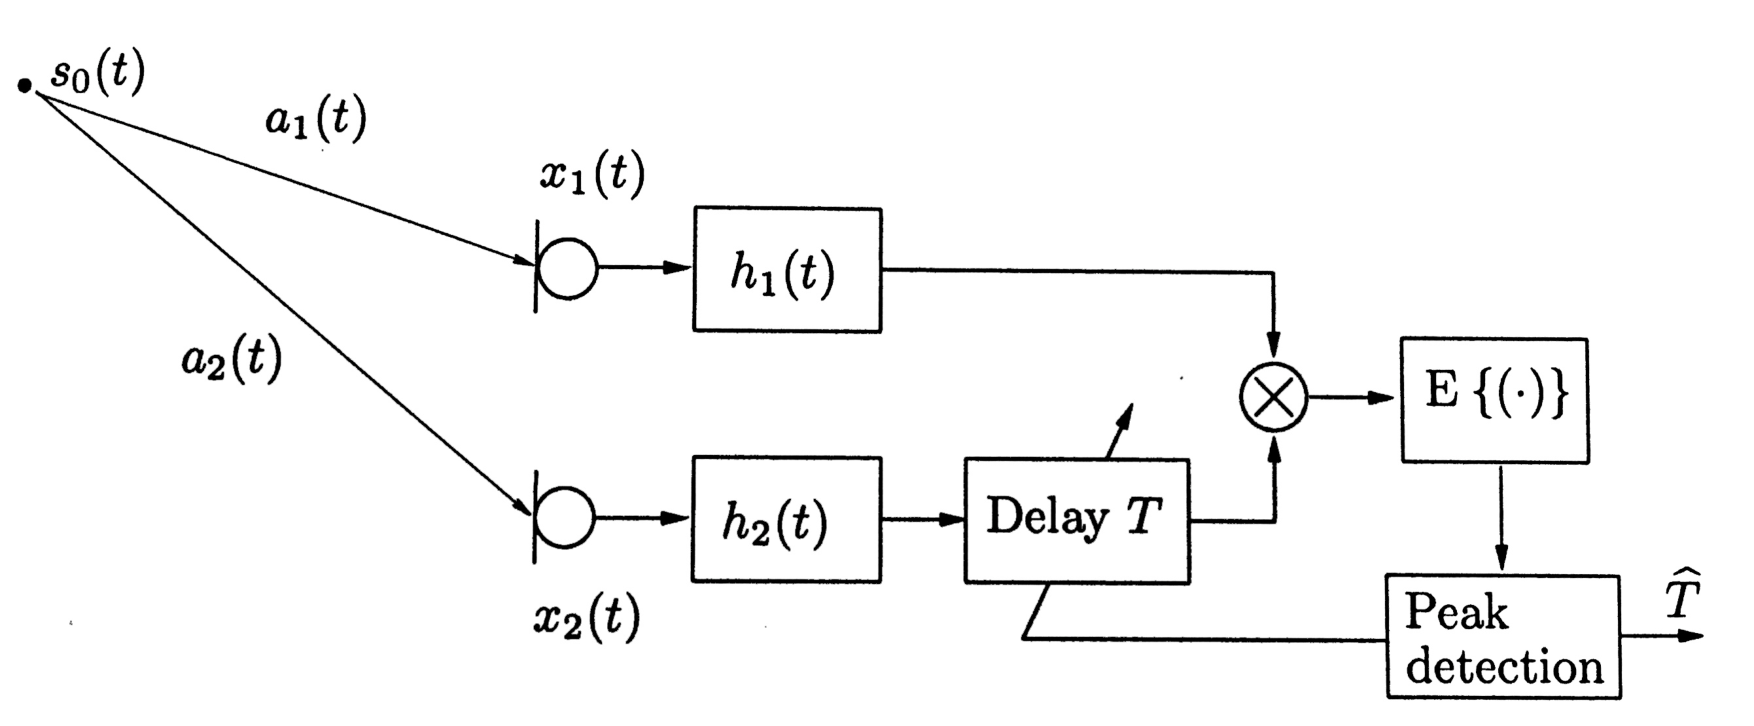
\includegraphics[width=0.80\textwidth]{figures/gcc.pdf}
% 	\caption{GCC}
% 	\label{fig:gcc}
% \end{figure}

\subsection{Minimum Variance Distortionless Response Filter}
\label{subsec:mvdr}
The \ac{MVDR} optimization criterion states that the output variance in equation \ref{eq:bf_power} shall be minimized, under the constraint of no distortion in steering direction $\theta$. This optimization can mathematically be described as

\begin{equation}
\begin{split}
\vect W^H(\Omega) \mat \Phi_{xx}(\Omega)\vect W(\Omega) \rightarrow \min_{\vect W(\Omega)} \\
\text{subject to } \vect W^H(\Omega) \vect D(\Omega,\theta) = 1,
\end{split}
\end{equation}

% \todo{Do I have to refer to \ref{fig:ula} or \ref{eq:realtive_IR}?}
% where $\phi_{yy}$ represents the power of \ref{eq:bf_power}, also stated as variance, at the output of the beamformer.
where $\vect D(\Omega,\theta)$ is the steering vector, which is calculated similarly to the modeled propagation vector $\vect A_q^\text{ff}(\Omega)$ and uses the \ac{TDOA} from equation \ref{eq:timedelay}: $\vect D(\Omega,\theta) = \exp(-j\Omega f_s \Delta \vect \tau(\theta))$. However, it represents the steering direction $\theta$ of the array and not the propagation direction $\varphi$ also called \ac{DOA} of the signal $S_q(\Omega)$. For convenience, the normalized frequency $\Omega$ is neglected but will be reintroduced when it is needed. The optimization may be solved using the technique of Lagrange multipliers \cite[Section~2,~Chapter~4]{lagrange}\cite[Chapter~6.2.5.6]{bronstein}, which results in
% \cite[Appendix~E]{bishop2016pattern}
\begin{equation}
\vect W_\text{CAP}(\theta) = \frac{\mat{\Phi}_{xx}^{-1} \vect D(\theta) } { \vect D^H(\theta) \mat{\Phi}_{xx}^{-1} \vect D(\theta) }.
\label{eq:w_capon}
\end{equation}

This beamforming technique is also known as Capon beamformer by the name of its inventor.
\cite{Capon1969,krim1996two}

%\todo{MVDR mit phiVV hier formulieren auf unterschiede hinweisen}

\subsection{Delay and Sum Beamformer}
\label{subsec:DS}
The \ac{DS} beamformer is a special case of the \ac{MVDR} beamformer.
The beamformer is optimized for the uncorrelated sound field as noise.
To derive the \ac{DS} beamformer, the optimization criterion has to be changed from minimizing the output power $\phi_{yy}$ to minimizing the noise after the beamformer weights $\vect W^H\mat \Phi_{vv}\vect W$.
%This is viable if the steering vector $D(\theta)$ is equal to propagation vector $\vect A_q(\phi)$. The derivation for this can be comprehended in the appendix (XXX). Employing this constraint the desired signal remains untouched in any case, which makes the beamformer more robust against deviation of the steering angle $\theta$ concerning the actual \ac{DOA}.
The resulting weight vector changes from \ref{eq:w_capon} to \footnote{Note that equation \ref{eq:w_capon} and \ref{eq:w_capon_mod} are equal only if $\vect D(\theta) = \vect A_q(\varphi)$. If the assumed steering vector $\vect D(\theta) \neq \vect A_q(\varphi)$, which is usually the case in realistic acoustic environments, equation \ref{eq:w_capon} will lead to signal distortions. Equation \ref{eq:w_capon_mod} on the other hand is more robust to steering vector mismatch as only the noise is minimized.}

\begin{equation}
\vect W(\theta) = \frac{\mat{\Phi}_{vv}^{-1} \vect D(\theta) } { \vect D^H(\theta) \mat{\Phi}_{vv}^{-1} \vect D(\theta) }. \label{eq:w_capon_mod}
\end{equation}

Assuming a spatial uncorrelated noise field, the noise power $\mat \Phi_{vv}$ reduces to a unit matrix $\mat \Phi_{vv} \rightarrow \phi_{vv} \mat I$. With this assumption used in \ref{eq:w_capon_mod}, the \ac{DS} weights can be stated as

\begin{equation}
\begin{split}
\vect W_\text{DS}(\theta) &= \frac{\phi_{vv} \vect D(\theta) } {\phi_{vv} \vect D^H(\theta)\vect D(\theta)  }\\
&= \frac{\vect D(\theta)}{M}. \label{eq:w_ds}
\end{split}
\end{equation}

The number of microphones $M$ is seen in the denominator because squaring reduces the steering vector, which consists of $M$ unit vectors to the number of elements. This beamformer can be seen as time compensation before the summation. Therefore the name \emph{delay \& sum} beamformer is used. \cite[Chapter~2]{brandstein2013microphone}

\section{Acoustic Speaker Localization}
\label{sec:localization}
% Direction-of-Arrival Estimation
The \ac{ASL} techniques known from literature can broadly be divided into two parts. On the one hand the parametric approach exists. Here a multidimensional search has to be deployed to find all estimates at once. One of the most frequently used parametric approaches is the \ac{ML} technique. On the other hand there are the spectral-based algorithms, which are computationally more feasible than the preceding one, but may suffer from inaccuracy. In this approach, a spectrum-like function is formed, which can be searched for the parameters of interest. Spectral-based methods can again be subdivided into beamforming and subspace-based techniques. One of the most popular subspace-based techniques is \ac{MUSIC}, which utilizes an eigenvalue decomposition, that again is computationally very complicated. Subspace-based techniques is a field of great research interests with the development of multiple techniques like CSSM \cite{1164667}, TOPS \cite{yoon2006tops}, FRIDA \cite{pan2017frida} or WAVES \cite{di2001waves}. In this work, the beamforming technique is used and will be discussed in more detail. \cite{krim1996two}

% - Spectra-based\\
% Subspace-based
\subsection{Steered Response Power}
\label{subsec:SRP}
The \ac{SRP} method tries to estimate the \ac{DOA} by steering a beamformer towards a set of possible directions and calculating the resulting power. In a second step, the angle that maximizes the power is chosen as the \ac{DOA} estimate. This method can be applied with different kinds of beamformers. \\
The output power of the Capon beamformer can be written by inserting \ref{eq:w_capon} in \ref{eq:bf_power} as

\begin{equation}
\begin{split}
P_\text{CAP}(\Omega,\theta) &= \vect W_\text{CAP}^H(\Omega, \theta) \mat \Phi_{xx}(\Omega)\vect W_\text{CAP}(\Omega, \theta)\\
&=
\frac{\vect D(\Omega, \theta)^H \mat{\Phi}_{xx}^{-1}(\Omega)  } { \vect D^H(\Omega, \theta) \mat{\Phi}_{xx}^{-1}(\Omega) \vect D(\Omega, \theta) }
\mat \Phi_{xx}(\Omega)
\frac{\mat{\Phi}_{xx}^{-1}(\Omega) \vect D(\Omega, \theta) } { \vect D^H(\Omega, \theta) \mat{\Phi}_{xx}^{-1}(\Omega) \vect D(\Omega, \theta) }\\
&=...\\
&=
\frac{1}{\vect D^H(\Omega, \theta)\ \mat{\Phi}_{xx}^{-1}(\Omega)\ \vect D(\Omega, \theta)}.
\end{split}
\label{eq:p_capon}
\end{equation}

% Here, the \ac{STFT} notation stated in \ref{} is reintroduced.
Respectively, when using \ref{eq:w_ds} in \ref{eq:bf_power}, the power output of the \ac{DS} beamformer can be stated as

\begin{equation}
P_\text{DS}(\Omega,\theta) = \frac{\vect D^H(\Omega, \theta)\ \mat{\Phi_{xx}}(\Omega)\ \vect D(\Omega, \theta)}{M^2}.
\label{eq:p_ds}
\end{equation}

% The results are also called spatial power spectrum because they are dependent on the frequency $\Omega$ and the steering direction $\theta$.\\
In the next step, the angle for the maximum steered power has to be found. This
can be done in two ways. The broadband method takes the mean over all frequencies and searches for the maximum afterwards. In the frequency \ac{DOA} estimation, the averaging over frequencies is dropped, and the maximum search is done  in every frequency.
% Before noting the mathematical equation for the broadband approach, the \ac{SRP-PHAT} shall be introduced. More robust localization were accomplished, when using the \emph{coherence} matrix instead of the covariance matrix. This change is done because the absolute power in every bin varies allot. The approach is, to normalize the covariance matrix by canceling out the absolute power and thus only the phase is holding all information, which is mathematically noted as
% \begin{equation}
% J_{xx}^{ij}(\Omega) = \frac{\phi_{ij}(\Omega)}{\sqrt{\phi_{ii}(\Omega)\phi_{jj}(\Omega)}},\; \forall i,j \in \{1,...,M\}
% \label{eq:coherence}
% \end{equation}
% where $J_{xx}^{ij}(\Omega)$ are the entries of the $M \times M$ coherence matrix $\mat J_{xx}$ and $\phi_{ij}$ are the elements of the covariance matrix $\mat \Phi_{xx}(\Omega)$. \\
% When using the coherence $\mat J_{xx}(\Omega)$ from \ref{eq:coherence} instead of the covariance $\mat \Phi_{xx}(\Omega)$ in \ref{eq:p_capon} and \ref{eq:p_ds} we obtain
% \begin{equation}
% P_\text{CAP,PHAT}(\Omega, \theta) = \frac{1}{\vect D^H(\Omega, \theta)\ \mat{J}_{xx}^{-1}(\Omega)\ \vect D(\Omega, \theta)},
% \label{eq:p_capon_phat}
% \end{equation}
% and
% \begin{equation}
% P_\text{DS,PHAT}(\Omega, \theta) = \frac{\vect D^H(\Omega, \theta)\ \mat{J}_{xx}(\Omega)\ \vect D(\Omega, \theta)}{M^2}.
% \label{eq:p_ds_phat}
% \end{equation}
The broadband method can be stated as following:
% By averaging the power over frequencies $\overline{P}^\text{b}(\theta)$,  and taking the $\arg \max$, the \ac{DOA} as a broadband estimate is finally obtained

% - SRP-PHAT DS\\
% - SRP-PHAT Capon\\
% %\subsection{Multi-source DOA}
% Broadband\\

\begin{equation}
\begin{split}
\hat{\varphi} &= \arg \max_{\theta}\frac{1}{2\pi}\int^\pi_{-\pi}P(\Omega,\theta)\mathrm{d}\Omega\\
 &= \arg \max_{\theta} \overline{P}^\text{b}(\theta).
\end{split}
\label{eq:doa_est_broadband}
\end{equation}

When averaging across frequencies is neglected, it yields a \ac{DOA} estimate for every frequency, which is noted as

\begin{equation}
\hat{\varphi}(\Omega) = \arg\max_{\theta}P(\Omega,\theta).
\label{eq:doa_est_freq}
\end{equation}

Receiving one value per frequency may enable a real multi-source detection, under the assumption, that the sources are spectrally disjoint. Broadband and frequency SRP values are distinguished by the dependence on frequency $\Omega$.
The broadband \ac{SRP} may also be weighted before mean taking. This can be done in different ways. One of them is the \ac{PHAT}. Mathematically this can be stated as

\begin{equation}
\begin{split}
\hat{\varphi} &= \arg \max_{\theta}\frac{1}{2\pi}\int^\pi_{-\pi}\frac{1}{\phi_{xx}(\Omega)}P(\Omega,\theta)\mathrm{d}\Omega\\
 &= \arg \max_{\theta} \overline{P}^\text{b}_\text{PHAT}(\theta).
\end{split}
\label{eq:doa_est_broadband_phat}
\end{equation}
The \ac{PHAT} weighted steered mean power is stated as $ \overline{P}^\text{b}_\text{PHAT}(\theta)$. It is assumed that the sound field is homogeneous, which means that the microphones have the same amount of variance $\phi_{xx}(\Omega)$.\footnote{Note that the variance $\phi_{xx}$ are the values on the main diagonal of the covariance matrix} Furthermore, the assumption decreases the computational load.
% \begin{equation}
% \begin{split}
% \phi_{ii} &= \phi_{jj}, \; \forall \ i,j \in \{ 1...M| i \neq j\}\\
%  &= \phi_{xx},
% \end{split}
% \label{eq:assumtion_homogen}
% \end{equation}
% where $\phi_{ii}$ and $\phi_{jj}$ are the values on the main diagonal of the covariance matrix.
This weighting leads to canceling out the absolute power. Thus only the phase is holding all information, and all spectral parts are having equal share in the broadband \ac{SRP} in respect to the mean. \cite[Chapter~8]{brandstein2013microphone}\cite{madhu2008scalable}\\

% \begin{figure}[!ht]
% 	\centering
% 	\includegraphics[width=0.45\textwidth]{figures/SPS_compare.png}
% 	\caption{Comparison}
% 	\label{fig:comparision}
% \end{figure}

\subsection{Theoretical Steered Power Spectrum and Aliasing}


The theoretical Steered Power Spectrum can be used to evaluate different types of beamformers. They are calculating the response of a microphone array to a wavefront with a certain \ac{DOA} for all parameters. As stated in chapter \ref{chap:introduction} in this work only the azimuth-plane is considered. So the response is dependent on the azimuth angle $\theta$ and the normed frequency $\Omega$. The theoretical steered power spectrum can be calculated, when considering a signal as in \ref{eq:sig_model_relativ} but with neglecting the noise $\vect V(\Omega) = 0$ and setting the modified source signal $S'(\Omega) = 1$ which can be seen as a white noise signal. %The response is then obtained when calculating the output power of the beamformer in decibel:
In dB, the \ac{SRP} then reads\footnote{Note that this is very similar to the well known beampattern. Here (equation \ref{eq:p_theory}), the beamformer weights are changed as apposed to changing $\vect A(\Omega)$ depending on $\theta$.}:

\begin{equation}
P_\text{theory}(\Omega,\theta) \mid _\text{db} = -10\log_{10}(|\vect W^H(\Omega,\theta)\vect A(\Omega)|^2).
\label{eq:p_theory}
\end{equation}

Different beamformer weight vectors $\vect W(\Omega,\theta)$ can be compared, for instance those of \ac{DS} beamformer \ref{eq:w_ds} or Capon beamformer \ref{eq:w_capon}. Steering vector $\vect D(\Omega,\theta)$ and propagation vector $\vect A(\Omega)$ are dependent on the array geometry and can for example be calculated with \ref{eq:ula} and \ref{eq:uca_c} in \ref{eq:transfer_free_field}. \cite[Chapter~2]{brandstein2013microphone}
Referring to these beamformers the theoretical steered power spectra for an \ac{UCA+C} arrangement are shown in figure \ref{fig:beampattern}. When comparing both spectra, it is observed that the spectrum for the Capon beamformer is much more distinct than the one for the \ac{DS} beamformer. However, in both plots the \ac{DOA} $\varphi = \ang{180}$ is visible. Mathematically the \ac{DOA} can be obtained by employing $P_\text{theory}(\Omega,\theta)$ in \ref{eq:doa_est_broadband} for broadband \ac{DOA} or in \ref{eq:doa_est_freq} frequency \ac{DOA}. \\
\label{subsec:pattern_aliasing}
\begin{figure}[!ht]
	\subfloat[\ac{SRP-PHAT} Delay \& Sum\label{fig:beamp_ds}]{%
		  \def\svgwidth{.48\linewidth}
		  \scriptsize\input{figures/beampattern_ds.pdf_tex}
	}
	\hfill
	\subfloat[\ac{SRP-PHAT} Capon\label{fig:beamp_capon}]{%
		  \def\svgwidth{.48\linewidth}
		  \scriptsize\input{figures/beampattern_capon.pdf_tex}
	}
	\caption{Theoretical steered power spectrum of a 7 microphone uniform circular array with center microphone with a \SI{42}{\milli\meter} radius. The direction of arrival $\phi$ of the acoustic signal is $\ang{180}$. Grating lobes at $\ang{60}$ and $\ang{300}$ are visible due to spatial aliasing.}
	\label{fig:beampattern}
\end{figure}
Another observation from figure \ref{fig:beampattern} concerns the so called \emph{grating lobes} in the upper frequencies at $\ang{60}$ and $\ang{300}$ azimuth angle $\theta$. Reason is the spatial aliasing, which occurs when the microphone distance is greater than half of the sound's wavelength. The grating lobes have the same amount of power as the main lobe and therefore cannot be distinguished by the \ac{SRP} algorithm when looking at single frequency bands. Aliasing is not only impacting the DOA estimation in specific frequencies but also the broadband \ac{SRP} when it is desired to detect more than one source. For example, when multiple sources are present, and one source is more active than the other, one cannot decide between a second source which is less active or the power peak stimulated by aliasing of the first source.\\
To illustrate the \ac{SRP} localization algorithm and how aliasing affects the localization, two polar plots are shown in figure \ref{fig:polar_doa}. In plot \ref{fig:polar_doa_broad} the broadband power $\overline{P}^\text{b}(\theta)$ is shown for the spectrum depicted in figure \ref{fig:beamp_ds}. This spectrum is used in \ref{eq:doa_est_broadband} to estimate the \ac{DOA}. Here, the \ac{DOA} of $\varphi = \ang{180}$ is also visible. The aliasing has only a small impact in the broadband power spectrum. The spatial power spectrum $P(\Omega, \theta)$ for different frequencies, like it is used in \ref{eq:doa_est_freq} to estimate \ac{DOA} per frequency, is shown in \ref{fig:polar_doa_sub}. In that figure, the \ac{DOA} can be obtained for the lower frequencies ($f = \SI{2}{\kilo \Hz}$, $f = \SI{4}{\kilo \Hz}$). However, for $f = \SI{6}{\kilo \Hz}$ grating lobes on the basis of aliasing occur massively, and are due to this ambiguity disqualifying the \ac{DOA} obtained with this frequency. Furthermore, it is visible that the main lobe becomes narrower in the upper frequencies which in contrary may lead to a more precise \ac{DOA} estimation.


\begin{figure}[!ht]
	\subfloat[\label{fig:polar_doa_broad}]{%
    	\def\svgwidth{.45\linewidth}
    	\scriptsize\input{figures/polar_doa_broad.pdf_tex}
	}
	\hfill
	\subfloat[\label{fig:polar_doa_sub}]{%
    	\def\svgwidth{0.45\linewidth}
    	\scriptsize\input{figures/polar_doa_sub.pdf_tex}
	}
	\caption{Polar plots for the theoretical steered power spectrum from figure \ref{fig:beamp_ds}. In (a) broadband power spectrum $\overline{P}(\theta)$ is plotted and in (b) the spatial power spectrum $P(\Omega,\theta)$ for different frequencies $f$ are plotted.
	Red: $f = \SI{2}{\kilo \Hz}$, Blue: $f = \SI{4}{\kilo \Hz}$, Green: $f = \SI{6}{\kilo \Hz}$}
	\label{fig:polar_doa}
\end{figure}



\subsection{Practical Realization}
\label{subsec:prac_real}
In practice some adjustments and assumptions are made to reduce the processing time or to make algorithms more robust. The latter is the reason to adjust the Capon beamformer (Equation \ref{eq:p_capon}). The main problem is that the covariance matrix may be singular and therefore the inverse of the matrix may not exist. Reason for the singular matrix may be, that fewer sources are dominant as the number of microphones. Thus the spatial covariance matrix has no full rank. The singularity problem can be fixed by a technique called diagonal loading. This is done by adding a small component $\epsilon$ to the main diagonal. Now the weights of the modified Capon beamformer reads as

\begin{equation}
\vect W'_\text{CAP}(\Omega,\theta) = \frac{({\mat{\Phi}}_{xx}(\Omega)+\epsilon\mat I)^{-1} \vect D(\Omega,\theta) } { \vect D^H(\Omega,\theta) ({\mat{\Phi}}_{xx}(\Omega)+\epsilon\mat I)^{-1} \vect D(\Omega,\theta) },
\label{eq:w_diag_load}
\end{equation}

where $\mat I$ is the unit matrix.
% For the power calculation, needed for the \ac{SRP} localization, \ref{eq:w_diag_load} is  encapsulated in \ref{eq:bf_power}, which results in
% \begin{equation}
% P'_\text{CAP} = \frac{\vect D^H(\theta) (\mat{\Phi}_{xx}+\epsilon\mat I)^{-1} \;{\mat{\Phi}}_{xx} \; (\mat{\Phi}_{xx}+\epsilon\mat I)^{-1}\vect D(\theta) }{(\vect D^H(\theta) (\mat{\Phi}_{xx}+\epsilon\mat I)^{-1} \vect D(\theta))^2}.
% \label{eq:p_diag_load}
% \end{equation}
%which is a much more complex calculation in comparison to \\\ref{}
%To reduce the effort, the matrix inversion could also be handled by a recursive MSE inversion which is much less intensive. \\
% In this work another simplification is made to reduce processing load when calculating the coherence matrix. It is assumed that the sound field is homogeneous, which means the microphones have the same amount of variance, denoted as
% \begin{equation}
% \begin{split}
% \phi_{ii} &= \phi_{jj}, \; \forall \ i,j \in \{ 1...M| i \neq j\}\\
%  &= \phi_{xx},
% \end{split}
% \label{eq:assumtion_homogen}
% \end{equation}
% where $\phi_{ii}$ and $\phi_{jj}$ are the values on the main diagonal of the covariance matrix. When using this in \ref{eq:coherence}, the following can be concluded for the coherence matrix
% \begin{equation}
% \mat J_{xx}(\Omega) = \frac{\mat \Phi_{xx}(\Omega)}{\mat \phi_{xx}(\Omega)}.
% \label{eq:coherence_mod}
% \end{equation}
% For the \ac{SRP-PHAT} localization, the coherence matrix $\mat J_{xx}(\Omega)$ shall also get diagonal loading when using the Capon beamformer.
However, the impact of the weighting in \ref{eq:w_diag_load} is heavily depended on the absolute values in covariance matrix ${\mat{\Phi}}_{xx}(\Omega)$. To cancel out the dependencies the so called coherence matrix is taken instead:

\begin{equation}
J_{xx}^{ij}(\Omega) = \frac{\phi_{ij}(\Omega)}{\sqrt{\phi_{ii}(\Omega)\phi_{jj}(\Omega)}},\; \forall i,j \in \{1,...,M\} ,
\label{eq:coherence}
\end{equation}

where $J_{xx}^{ij}(\Omega)$ are the entries of the $M \times M$ coherence matrix $\mat J_{xx}(\Omega)$ and $\phi_{ij}(\Omega)$ are the elements of the covariance matrix $\mat \Phi_{xx}(\Omega)$.
% The change from covariance to coherence matrix will later cancle out ...
When doing the diagonal loading on the coherence matrix, one wants to preserve the magnitude of one on the main diagonal, so instead of increasing the main diagonal by a small amount $\epsilon$ all other elements are decreased:

\begin{equation}
J'^{ij}_{xx}(\Omega) =
	\begin{cases}
		\frac{\mat \Phi_{xx}^{ij}(\Omega)}{\mat \phi_{xx}(\Omega)(1+\epsilon)}& i,j \in \{1...M\ |\  i \neq j\}\\
		\frac{\mat \Phi_{xx}^{ij}(\Omega)}{\mat \phi_{xx}(\Omega)} & i,j \in \{1...M\ |\  i = j\}
	\end{cases}.
\end{equation}
The loaded coherence matrix is then used in \ref{eq:w_capon} as $\mat \Phi_{xx}(\Omega)$ to gain the beamformer weights:
\begin{equation}
\vect W''_\text{CAP}(\Omega,\theta)= \frac{J'_{xx}(\Omega)^{-1} \vect D(\Omega,\theta)}{\vect D^H(\Omega,\theta)J'_{xx}(\Omega)^{-1} \vect D(\Omega,\theta)}
\label{eq:w_diag_load_coherence}
\end{equation}

Equation \ref{eq:w_diag_load_coherence} may be incorporated in \ref{eq:bf_power} to obtain the power
\begin{equation}
P''_\text{CAP}(\Omega, \theta) =
\frac{\vect D^H(\Omega,\theta) \mat J'^{-1}_{xx}(\Omega) \;{\mat{\Phi}}_{xx}(\Omega) \; \mat J'^{-1}_{xx}(\Omega) \vect D(\Omega,\theta)}
{\big(\vect D^H(\Omega,\theta) \mat J'^{-1}_{xx}(\Omega) \vect D(\Omega,\theta)\big)^2}.
\label{eq:p_diag_load_coherence}
\end{equation}
This method is also stated in \cite[Chapter~2]{brandstein2013microphone}.\\
A further adjustment has to be done because in real-time applications the incoming stream of data requires frame-wise processing. Another reason is the non-stationarity of speech and \ac{DOA}. This can be omitted when  considering only a short segment of microphone signals. As a result the $L$-point discrete Fourier transform is utilized, with an overlapping window function:

\begin{equation}
X(l,b) = \sum_{n=0}^{L-1}\mathcal{W}(n)x(bO+n)e^{-j2\pi n\frac{l}{L}}.
\end{equation}
The $l$ is the discrete frequency bin, $\mathcal{W}(n)$ is the window function, $O$ represents the frameshift in samples, and $b$ is the frame index. This method is called the \ac{STFT}. \cite[Chapter~2.5.4]{loizou2013speech} \\
Based on the \ac{STFT}, the equations \ref{eq:doa_est_broadband} and \ref{eq:doa_est_freq} changes as follows

\begin{equation}
\begin{split}
\hat{\varphi}(b) &= \arg \max_{\theta}\sum^{L/2}_{l=0}P(l,b,\theta)\\
&= \arg \max_{\theta}\overline P^\text{b}(b,\theta),
\end{split}
\label{eq:doa_est_broadband_stft}
\end{equation}

\begin{equation}
\hat{\varphi}(l,b) = \arg \max_{\theta}P(l,b,\theta).
\label{eq:doa_est_freq_stft}
\end{equation}

The \ac{DOA} estimate $\hat \varphi$ now depends on the discrete frequency $l$ and the frame index $b$. Due to symmetry properties only the frequency bins from 0 to $L/2$ are used.
%Therefore, for every of the $O=\frac{L}{2}-1$ sample a localization result is obtained.
Furthermore, the frame dependent \ac{SRP} is now called sub-band SRP, because of the sub-band frequency division by \ac{STFT}.\\
Furthermore, the effort to calculate the spatial covariance matrix can be reduced by only considering $B_E$ frames which may according to \cite{krim1996two}
be stated as

 % $\mat{\Phi}_{xx}$. The matrix has to be estimated given the samples $\vect \theta(\Omega,1),...,\vect \theta(\Omega,N)$. Therefore the covariance matrix $\mat{\hat{\Phi}}_{xx}$ may be stated as

\begin{equation}
\mat{ \hat{\Phi}}_{xx}(l,b) = \ex{\vect{X}(l,b)\vect{X}(l,b)^*} = \frac{1}{B_E}\sum^{B_E}_{b=1} \vect{X}(l,b)\vect{X}^H(l,b).
\end{equation}


A further simplification of the covariance matrix estimation is to use a first order \ac{IIR} filter, which can be noted as \\

\begin{equation}
\mat{\hat{\Phi}}_{xx}(l,b) = \alpha \mat{\hat{\Phi}}_{xx}(l,b-1)+(1-\alpha)\vect{X}(l,b)\vect{X}^H(l,b),
\label{eq:cross_iir}
\end{equation}
where $\alpha$ is the smoothing constant.
% For convenience the following chapters will still use the spatial covariance matrix, but it shall be stated that in reality it estimate is used.



%\subsection{Multiple Signal Classification}
%Subspace based approach Multiple Signal Classification

%\section{Speech Source Number Estimation}
\section{Source Classification with GMMs}
\label{sec:source_classification}
From chapter \ref{sec:localization} and the equations \label{eq:doa_est_broad_stft} and \ref{eq:doa_est_freq_stft} 'raw' localization date $\hat \varphi$ are resulting. Based on this data a robust localization for multiple sound sources shall be obtained. To perform multi-source localization, these raw results $\hat \varphi$ have to be classified. In other words, the parameters of the underlying model that represent the observations shall be estimated. This can be done by many different algorithms like \ac{kNN}, \ac{ANN} or \ac{SVM}. Another often used approach is a \ac{GMM}. This method forms a statistical model with the use of a mixture of Gaussian \acp{PDF}. \acp{GMM} have an advantage against \ac{kNN} because they do not need to store a large set of data, but only the statistical model. \cite[Chapter~17.2.3]{martin2008advances} \\

\subsection{Gaussian Mixture Models}
\label{subsec:GMM}
In the following, the basics of modeling data with a GMM are explained. The observations are the estimated \acp{DOA} $\hat \varphi$ in the azimuth plane. It is assumed that these observations have an underlying stochastic process, which shall be modeled by a set of one dimensional Gaussians. A single Gaussian \ac{PDF} can be written in this form

\begin{equation}
\mathcal{N}(\hat{\varphi}|\mu,\sigma)=\frac{1}{\sigma\sqrt{2\pi}}e^{-\frac{1}{2}(\frac{\hat{\varphi}-\mu}{\sigma})^2},
\end{equation}

where $\sigma$ is the standard deviation and $\mu$ the mean of the Gaussian.
To get a \ac{GMM} one needs to form a linear superposition of $K$ Gaussians stated as

\begin{equation}
p_{\text{GMM}}(\hat{\varphi}|\vect \mu,\vect \sigma,\vect \pi)= \sum^K_{k=1}\pi_k\mathcal{N}(\hat{\varphi}|\mu_k,\sigma_k).
\label{eq:gmm}
\end{equation}

where $\vect \mu = \{\mu_1, \mu_k,...,\mu_K \}$, $\vect \sigma = \{\sigma_1, \sigma_k,...,\sigma_K \}$ and $\vect \pi = \{\pi_1, \pi_k,...,\pi_K \}$ are sets of means, standard deviations and mixing coefficients for every class $k$. The mixing coefficients are used to normalize the \ac{GMM} \ac{PDF}. One of the main properties of a \ac{PDF} is that the integral over its variable has to be one $\int_{\hat \varphi} p(\hat \varphi) \mathrm{d} \varphi =1$. Therefore, the sum over all  single mixing coefficients $\pi_k$ must also be one and in the range between zero and one for any $k$, which can be stated as

\begin{equation}
\sum^K_{k=1}\pi_k = 1, \ \ \ \ 0 \leqslant \pi_k \leqslant 1.
\label{eq:pi_constraint}
\end{equation}

% \cite{wiki}
\subsection{Parameter Estimation}
\label{subsec:parameter_est}

At first hand, the GMM is not a classification algorithm, but rather a method to model data.
If it is known to which class a given observation belongs to (the representations of every observation is known), one can separate this superposition of Gaussians into an estimation of $k$ single Gaussians. This can be done with the help of the \ac{ML} estimators,

\begin{equation}
\begin{split}
\mu_k &= \frac{\sum^{N_k}_{n=1}\hat{\varphi}_n}{N_k}\\
\sigma_k &= \frac{1}{N_k}\sum^{N_k}_{n=1}(\hat{\varphi}_n-\mu_k)^2,
\end{split}
\end{equation}

where the data set consists of $\vect{\hat{\varphi}} = \{\hat{\varphi}_1,...,\hat{\varphi}_{N_k}\}$ observations, $N_k$ is the number of data which are representatives of class $k$.
However, if the information about a class representation is not observable, the parameter cannot be estimated by a closed form solution. Unknown representations are also called latent variables. This problem can be stated as the joint probability of \ref{eq:gmm} over all $N$ observations $\vect{\hat{\varphi}} = \{\hat{\varphi}_1, \hat{\varphi}_n,...,\hat{\varphi}_N \}$

\begin{equation}
p_\text{GMM}(\vect{\hat{\varphi}}|\vect \mu,\vect \sigma, \vect \pi) = \prod^{N}_{n=1}\Bigg[\sum^K_{k=1}\pi_k\mathcal{N}( \hat{\varphi}_n|\mu_k,\sigma_k)\Bigg] \rightarrow \max,
\label{eq:ML}
\end{equation}
where $p_\text{GMM}(\vect{\hat{\varphi}}|\vect \pi,\vect \mu,\vect \sigma) $ is the joint likelihood how probable the observations $\vect {\hat \varphi}$ are given the model consisting of $\vect \pi,\vect \mu$ and $\vect \sigma$. This likelihood shall be maximized, which is also known as \ac{ML} estimation. Alternatively, the logarithmic probability can be maximized

\begin{equation}
\ln p_\text{GMM}(\vect{\hat{\varphi}} |\vect \mu,\vect \sigma, \vect \pi) = \sum^{N}_{n=1}\ln\Bigg\{\sum^K_{k=1}\pi_k\mathcal{N}(\hat{\varphi}_n|\mu_k,\sigma_k)\Bigg\} \rightarrow \max.
\label{eq:log_ML}
\end{equation}

Finding the \ac{ML} solution for a \ac{GMM} with latent variables can be accomplished using the \ac{EM}-algorithm, which is a recursive process, as illustrated in figure \ref{fig:EM}. First, the parameter set has to be initialized as seen in figure \ref{fig:EM}.a. This can be done randomly or with an educated guess. Afterwards, the recursive process starts with the expectation step, where the latent variables for each observation $\hat{\varphi}_n$ are estimated (figure \ref{fig:EM}.a). They are called responsibilities $\gamma_{kn}$ and may be expressed as

\begin{equation}
\gamma_{kn} = \frac{\pi_k \mathcal{N}(\hat{\varphi}_n|\mu_k,\sigma_k)}{\sum^K_{k'=1} \pi_{k'}\mathcal{N}(\hat{\varphi}_n|\mu_{k'},\sigma_{k'})} = \frac{p_k(\hat{\varphi}_n)}{p_\text{GMM}(\hat{\varphi}_n|\vect \mu,\vect \sigma, \vect \pi)},
\label{eq:em_gamma}
\end{equation}

where $p_k$ represents a single Gaussian \ac{PDF} of class $k$. The calculation of these responsibilities can also be comprehended in figure \ref{fig:EM_1}. Here you can see that the total probability $p_{GMM}(\phih)$ (red) will be set into relation to the single probabilities $p_1(\phih)$ or $p_2(\phih)$ (blue or teal) to result in the responsibilities $\gamma_1$ or $\gamma_2$. In the overview figure \ref{fig:EM} the estimation of responsibilities in (b) is shown as a coloration of the observations in class colors.

\begin{figure}[!ht]
	\centering
    \def\svgwidth{1\linewidth}
    \scriptsize\input{figures/gamma_1.pdf_tex}
	\caption{In plot (a) the probability density function for two classes and the total Gaussian mixture model distribution is shown. In plot (b) the resulting responsibilities are shown, which are calculated by dividing a single probability density function by the the total distribution.}
	\label{fig:EM_1}
\end{figure}
%Responsibilities are also referred to as the a posterior probability.

Next, in the maximization step, the parameters of the \ac{GMM} are estimated (figure \ref{fig:EM_1}.c). The \ac{ML} estimation of the mean $\mu_k$ can be written as

\begin{equation}
\mu_k = \frac{\sum^N_{n=1}\gamma_{kn}\hat{\varphi}_n}{N_k},
\label{eq:mu_em}
\end{equation}

where $N_k$ is the number of observations associated with class $k$

\begin{equation}
N_k = \sum^N_{n=1} \gamma_{nk}.
\end{equation}

It can be noted that this estimation for every class $k$ is a weighted mean of all $N$ observations in the set. The standard deviation can be written as

\begin{equation}
\sigma_k = \frac{1}{N_k}\sum^N_{n=1}\gamma_{kn}(\hat{\varphi}_n-\mu_k)^2.
\label{eq:sigma_em}
\end{equation}

Last, the mixing coefficients are stated as

\begin{equation}
\pi_k = \frac{\sum^N_{n=1}\gamma_{kn}}{N}.
\label{eq:pi_em}
\end{equation}

After the maximization step is done, the recursive algorithm has to evaluate if it has to do another iteration $I$ on the set $\vect{\hat{\varphi}}$ of observations or to terminate the algorithm. This may be done by evaluation if the log likelihood in \ref{eq:log_ML} is converging. If the convergence criterion is not satisfied, the algorithm shall be starting again at the expectation step. A full derivation of the \ac{EM}-algorithm can be found in \cite[Chapter~9.2]{bishop2016pattern}.

\begin{figure}[!ht]
	\centering
		  \def\svgwidth{1\linewidth}
		  \scriptsize\input{figures/EM.pdf_tex}
	\caption{Parameter estimation of a two dimensional Gaussian mixture model using an expectation-maximization algorithm according to \cite[Chapter~9.2.2]{bishop2016pattern}. After the initialization (a), the responsibilities to the classes for the observations are calculated in the E-step (b). Based on the responsibilities, the \acl{GMM} parameter are recalculated in the M-step (c). Step (b) and (c) are repeated in every iteration $I$, till the log likelihood in \ref{eq:log_ML} is converging (f).}
	\label{fig:EM}
\end{figure}

\subsection{Use of Wrapped Gaussian Mixture Model for Periodic Observations}
\label{subsec:wgmm}
Since this work is restricted to the use of circular arrays
(stated in chapter \ref{chap:introduction}), the \ac{GMM} has to deal with cyclic observations. For instance, there are two observations given at $\hat{\varphi}_1 = \ang{359}$ and  $\hat{\varphi}_2 = \ang{1}$ and they should be modeled as one Gaussian distribution. With the \ac{ML} estimator for standard deviation \ref{eq:sigma_em} this gives different results of the underlying Gaussian distribution than the observations on the other side of the circle ($\hat{\varphi}_3 = \ang{179}$ and $\hat{\varphi}_4 = \ang{181}$). This inconsistency problem has to be handled with a new approach. One approach could be the von-Mises-distribution, which can be derived by taking a two-dimensional Gaussian and map it onto the unit circle. Von Mises distribution has the drawback that it makes use of the Bessel function which can be quite complex to handle when deriving the \ac{ML}-estimators. Another approach is the wrapped Gaussian, which is defined as a $2\pi$ periodical recurrent Gaussian.

\begin{equation}
\mathcal{N}_\text{w}(\hat{\varphi}|\mu,\sigma)=\frac{1}{\sigma\sqrt{2\pi}}\sum^\infty_{i=-\infty}e^{-\frac{1}{2}(\frac{\hat{\varphi}-\mu+2\pi i}{\sigma})^2},\ \phih \in [0,..,2\pi).
\label{eq:wrapped_dist}
\end{equation}



% with
% \begin{equation}
% \{ x \in \mathds{R} \text{ } | \text{ } 0 \leq x \leq 2\pi \}
% \end{equation}

This corresponds to 'wrapping' the real axis around the unit circle. Finally, incorporating \ref{eq:wrapped_dist} in \ref{eq:gmm} results in an \ac{WGMM}. \cite[Chapter~2.3.8]{bishop2016pattern}

\section{State of the Art}
\label{sec:state_of_art}

Multi-source localization is an active field of research. It can be separated in approaches which use distributed microphone networks \cite{brutti2008localization,sheng2005maximum,hummes2011robust} or approaches that use compact arrays. This work focuses on the compact arrays that can be integrated in smart speakers. In this section, first the general state is given for localization with compact arrays. Then an algorithm which utilizes also a \ac{GMM} from Nilesh Madhu is described in more detail. This algorithm will be used later as an external reference algorithm.

\subsection{General State}
In most papers a general strategy is to utilize first a core localizing technique to get raw localization results. Afterwards the data are used by a post-processing algorithm to separate the results into classes. The post-processing may also be a tracking algorithm integrated like a Kalman-Filter or a particle filter. In figure \ref{fig:general_overview} this approach is depicted.

\tikzset{
>=stealth',
  punktchain/.style={
    rectangle,
    rounded corners,
    fill=black!10,
    draw=black, very thick,
    text width=6em,
    minimum height=3em,
    text centered,
    on chain},
  line/.style={draw, thick, <-},
  element/.style={
    tape,
    top color=white,
    bottom color=blue!50!black!60!,
    minimum width=4em,
    draw=blue!40!black!90, very thick,
    text width=4em,
    minimum height=3.5em,
    text centered,
    on chain},
  every join/.style={->, thick,shorten >=1pt},
  decoration={brace},
  tuborg/.style={decorate},
  tubnode/.style={midway, right=2pt},
}

\begin{figure}[!ht]
	\centering
\begin{tikzpicture}
  [node distance=1cm,
  start chain=going right,]
     \node[punktchain, join, draw=none, fill=none] (audio) {Audio Signal};
     % \node[punktchain, join] (stft)      {STFT};
     \node[punktchain, join] (loc)      {Localization\\ Method};
     \node[punktchain, join] (post) {Post\\ Processing};
     \node[punktchain, join, draw=none, fill=none] (beamforming){Classified Localization Results};
\end{tikzpicture}
	\caption{Block diagram for the general principal of multi-source localization.}
	\label{fig:general_overview}
\end{figure}

An interesting real-time approach for circular arrays was made by Pavlidi et al.. They transform the signal with a Fourier transform to have the time-frequency representation. Here they are searching for \emph{single source} zones, where only one source is active. Therefore, they can use a single source \ac{DOA} algorithm over these zones by searching maximums over the so called \ac{CISC} which is quite similar to the \ac{SRP} method. From this they generate a smoothed histogram of \ac{DOA} estimations. Finally they employ a method, called \emph{matching pursuit}, to estimate the number of active sources and the corresponding \acp{DOA}. \cite{pavlidi2013real}\\
Another method by Jean-Mark Valin et al. was created for detecting simultaneously moving sound sources for a mobile robot. The array of 8 microphones is structured like a cube with one microphone on each corner. The strategy is also close to the general approach stated before. They use \ac{SRP} with a \ac{DS} beamformer and a spherical search grid to obtain a steered power spectrum. Afterwards they conduct a particle filter-based  post-processing which yields source positions. \cite{valin2007robust}\\
Nikunen at al. built a source separation which includes a multi-source localization algorithm. They use also \ac{SRP} as a core localizer and then classify the broadband steered power spectrum with an EM-Algorithm and a \ac{WGMM}. Afterwards they conduct a particle filter as a source tracking on the results of the EM-Algorithm.\cite{nikunen2018separation}\\
The research of Evers et al. concentrate on the post-processing with the \ac{GM-PHD} filters. This filter was developed for multi target tracking in presence of clutter and missing detections. \cite{evers2015bearing}

% \begin{figure}[!ht]
% 	\centering
% 	\includegraphics[width=\textwidth]{figures/nikunen_1.PNG}
% 	\caption{Nikunen}
% 	\label{fig:Nikunen}
% \end{figure}


% \begin{figure}[!ht]
% 	\centering
% 	\includegraphics[width=0.54\textwidth]{figures/matching_1.png}
% 	\caption{Matching Pursuit}
% 	\label{fig:matching}
% \end{figure}


\subsection{Madhu's Multi-source Localization Algorithm}
\label{subsec:madhu_alg}

Nilesh Madhu's multi-source localization algorithm is based as some others before on the \ac{SRP} with a \ac{DS} beamformer. He uses a \ac{ULA} and therefore can only detect values between $\ang{0}$ and $\ang{180}$ due to the symmetry of the array. It uses equation \ref{eq:doa_est_freq_stft} to obtain the localization results and buffers them over frequency $l$ in a frame $b$ which can be written as

\begin{equation}
\vect \phih(b) = \big(\phih(l_\text{low},b),...,\phih(L/2,b) \big)^T,
\end{equation}

where $l_\text{low}$ is a lower frequency bound. This excludes bins that are below this bound because low frequencies do not yield good localization estimates. Upon these data a \ac{GMM} is trained with an \ac{EM}-algorithm. This is done on a frame basis, so the index $b$ will be dropped till it is needed again. The general approach is to start the \ac{EM}-algorithm with an over-estimation for sources $K_\text{init}$. So the starting order of the system is $K\leftarrow K_\text{init}$. When this \ac{EM} is applied to the observations $\vect \phih(b)$ a fitted \ac{GMM} with means $\vect \mu$, variances $\vect \sigma^2$ and mixing coefficients $\vect \pi$ is obtained. Because of the overestimation the underlying process may be overdetermined and a \emph{shrinking} process is introduced, which reduces the model. This is done by limiting the distance of the mean estimated $\Gamma_\text{mean}^\text{dist}$. When this threshold is hit by two classes the classes are shrunken to one class by the following method:\\
if $\exists i,i'$, such that $|\mu_i-\mu_{i'}|\leq\Gamma_\text{mean}^\text{dist}$
\begin{equation}
\begin{split}
\mu_i &\leftarrow \frac{\pi_i\mu_i+\pi_{i'}\mu_{i'}}{\pi_i+\pi_{i'}}\\
\sigma^2_i &\leftarrow \frac{\pi_i\sigma^2_i+\pi_{i'}\sigma^2_{i'}}{\pi_i+\pi_{i'}}\\
\pi_i &\leftarrow \pi_i+\pi_{i'}\\
K &\leftarrow K-1.
\end{split}
\end{equation}

After the shrinking, the \ac{EM}-algorithm is used again with the \ac{GMM}
as initial values. This process is repeated till the separation of all mean values are at least $\Gamma_\text{mean}^\text{dist}$. The number of classes $K$ indicated the estimated number of sources. In addition to the \ac{GMM} a noise class is added. This is necessary due to random distributed observations in bins where no source is active. The floor class is modeled as a \emph{hidden component} $(K+1)$ with a constant mean $\mu_{K+1}=\ang{90}$ and a large standard deviation. For the hidden component, only the mixing coefficients and variance is adapted during the \ac{EM}-algorithm. The tracking is done with the help of an overlying \ac{GMM} ($\vect{\overline{\mu}}, \vect{\overline{\sigma^2}}, \vect{\overline{\pi}}$). The overlying \ac{GMM} has the purpose to handle the changing number of sources in the acoustic scene. Sometimes sources do speech pauses, new sources  arise, while others disappear and some are moving. This is not depicted in looking at single frames and therefore the overlying \ac{GMM} is used. To handle the 'death' of sources the \ac{TTL} $\overline b_{\text{TTL},k}$ is introduced. The update of the overlying \ac{GMM} for any time frame $b$ can be stated as the following:\\
If $\exists\ i, \overline i$, at frame $b$ such that $|\mu_i-\mu_{\overline i}|\leq\Gamma_\text{mean}^\text{dist}$

\begin{equation}
\begin{split}
\overline \mu_{\overline i} &\leftarrow \frac{\overline \pi_{\overline i}\overline \mu_{\overline i}+\pi_{i}(b)\mu_{i}(b)}{\overline \pi_{\overline i}+\pi_{i}(b)}\\
\overline\sigma^2_{\overline i} &\leftarrow \frac{\overline\pi_{\overline i}\overline\sigma^2_{\overline i}+\pi_{i}(b)\sigma^2_{i}(b)}{\overline\pi_{\overline i}+\pi_{i}(b)}\\
\overline\pi_i &\leftarrow \overline\pi_i+\pi_{i}(b)\\
\overline b_{\text{TTL},{\overline i}} &\leftarrow \min( \overline b_{\text{TTL},{\overline i}}(b)+1,\Gamma^\text{ max}_\text{TTL})
\end{split}
\label{eq:madhu_update}
\end{equation}

and for each $i$ in frame $b$ such that $\nexists \overline i$ , with  $|\mu_i-\mu_{\overline i}|\leq\Gamma_\text{mean}^\text{dist}$

\begin{equation}
\begin{split}
\overline \mu_{\overline i} &\leftarrow \overline \mu_{\overline i}\ \cup\ \mu_i(b)\\
\overline\sigma^2_{\overline i} &\leftarrow \overline\sigma^2_{\overline i}\ \cup\ \sigma^2_i(b)\\
\overline\pi_i &\leftarrow \overline\pi_i\ \cup\ \pi_i(b)\\
\overline b_{\text{TTL},{\overline i}} &\leftarrow b^\text{init}_\text{TTL}\\
\overline K &\leftarrow \overline K + 1\\
\end{split}
\label{eq:madhu_add}
\end{equation}

and for each $\overline i$ such that $\nexists i$ in frame $b$, with  $|\mu_i-\mu_{\overline i}|\leq\Gamma_\text{mean}^\text{dist}$

\begin{equation}
\overline b_{\text{TTL},{\overline i}} \leftarrow \overline b_{\text{TTL},{\overline i}}(b)-1.
\label{eq:madhu_decrease}
\end{equation}

The equations \ref{eq:madhu_update} state how the overlying \ac{GMM} class is updated by the current trained \ac{GMM} class, if their distances to each others are below the threshold $\Gamma_\text{mean}^\text{dist}$. If no overlying \ac{GMM} class is in distance to the current trained \ac{GMM} class then a new class is opened, which is stated in equation \ref{eq:madhu_add}. Equation \ref{eq:madhu_decrease} describes the decrease of the \ac{TTL} in the overlying \ac{GMM}, if no class of the current \ac{GMM} is present for updating. If $\overline b_{\text{TTL},{\overline i}} \leq 0$ the source is considered as \emph{died} and therefore will be removed from the system. The maximum \ac{TTL} threshold $\Gamma^\text{ max}_\text{TTL}$ is introduced to limit the source lifetime and $b_\text{TTL}\text{init}$ is considered as initial value for the \ac{TTL}. $\overline K$ is considered as the number of classes of the overlying \ac{GMM}. After this update the overlying \ac{GMM} renormalizes the mixing coefficient to guarantee the constraint \ref{eq:pi_constraint}. \cite{madhu2008scalable} \cite[Chapter~4.3]{madhu2010acoustic}

% \begin{figure}[!ht]
% 	\subfloat[Clustering\label{fig:madhu_1}]{%
% 	  \includegraphics[width=0.45\textwidth]{figures/madhu_1.png}
% 	}
% 	\hfill
% 	\subfloat[Graustufen und Marker\label{fig:madhu_2}]{%
% 	  \includegraphics[width=0.45\textwidth]{figures/madhu_2.png}
% 	}
% 	\caption{GMM, sum, noise class, single Gaussian}
% 	\label{fig:madhu}
% \end{figure}

\newpage
\endinput

%!TEX root = ../IfN-LaTex.tex
%!TEX spellcheck

\chapter[Adaptive EM-based Multi-source Localization Algorithm]{Adaptive EM-based Multi-source Localization Algorithm using a Wrapped Gaussian Mixture Model}
\label{chap:Proposed}

In this chapter, the developed multi-source localization method is described.
The core of this method is a \ac{GMM} which is estimated by an \ac{EM}-algorithm. The main challenges are the addition and deletion of new sources $q$ where each is represented by one Gaussian. Furthermore, the change from processing on a block of static data to the processing of varying real-time data has to be tackled, which is not covered by a classical \ac{EM}-algorithm. \\

\begin{figure}[!h]
	\centering
    \begin{tikzpicture}
	[
  	coordinate/.style={minimum height=1em,},
    rect2/.style={
    rectangle, 
    % fill=black!10,
    draw=black, thick,
    text width=8em, 
    minimum height=3em, 
    text centered
    },
	]
	\matrix (m1) [row sep=1em, column sep=2.7em]
	{
		\node[dspnodeopen, align=right]         		   	(phi) {\hspace{1em} $\vect{\hat{\varphi}}(b)$, \ref{sec:alg_localization}};  		&%
		\node[dspnodefull, xshift=1em]                   (node1) {};          		&
		\node[coordinate,text width=6em]                  	(emphi) {};				&
		\node[coordinate]                   () {};          		&
		\node[coordinate]                  	() {};				\\
		% \node[coordinate]                  	(m05) {};				\\
		% %--------------------------------------------------------------------
		\node[dspnodeopen]         		   	(conf) {\hspace{1em} $\vect c(b)$, \ref{sec:confidence}};  		&%
		\node[dspnodefull, xshift=-1em]                  	(node2) {};				&
		\node[coordinate,text width=6em]                  	(emc) {};				&
		\node[coordinate, minimum height=5em,text width=6em,] 	(del) {};				&
		\node[dspnodefull]                   (node3) {};          		&
		\node[dspnodeopen]                  				(out) {$\vect \lambda^\text{out}(b)$};				\\

		% %--------------------------------------------------------------------
		\node[coordinate]                  	() {};				&
		\node[rect2, label=above left:{\ref{sec:hyp_test}},text width=7em, minimum height=3em]                  	(hyp) {Detection of \\ new sources};				&
		\node[coordinate,text width=6em]                  	(emhyp) {};				&
		\node[coordinate]                  	() {};				&
		\node[coordinate]  					() {};				\\
		% %--------------------------------------------------------------------
		\node[coordinate]                  	() {};				&
		\node[coordinate]                  	() {};				&
		\node[dspfilter]                  	(z) {$\z^{-1}$};				&
		\node[coordinate]                  	() {};				&
		\node[coordinate]                  	() {};				\\
		% \node[dspnodeopen]         		   	(m20) {$s_Q[n]$};  		&
		% \node[dspfilter,minimum width=1.4cm]	(m21) {$h_{mQ}[n]$}; 	&
		% \node[dspadder]                    	(m22) {};          		&
		% \node[dspadder]                    	(m23) {};          		&
		% \node[dspmultiplier]			   	(m24) {};  %dsp/label=belo
		% \draw [line width=0.25mm] 
		% ([yshift=8pt]m24.west) -- ([yshift=-8pt]m24.west); 			&
		% \node[dspnodeopen] 	     		 	(m25) {$x_m[n]$}; 		\\

	\\
	};
	\node[dspfilter, inner sep=0.4em, label=above:{\ref{sec:update}}] (em) [fit=(emphi) (emhyp) ,text width=6em ] {GMM Variables Update};
	\node[dspfilter, inner sep=0.0em, label=above:{\ref{sec:del}}] (delout) [fit=(del), text width=6em ] {Deletion of inactive sources};

	% \node[dspfilter,minimum width=1.4cm]	(m02) {EM Algorithm}; 	&
	\draw[dspconn] (phi) -- (emphi.west);
	\draw[dspconn] (conf) -- (emc.west);
	\draw[dspconn] (hyp) -- node [above]  {$\vect \lambda^\text{in}(b)$} (emhyp.west);
	\draw[dspconn] (emc) -- node [above]  {$\vect \lambda(b)$} (delout);
	\draw[dspconn] (node3) |- node [above left]  {$\vect \lambda^\text{out}(b)$} (z);
	\draw[dspconn] (z) -| node [above right]  {$\vect \lambda^\text{old}(b)$} (hyp);
	\draw[dspconn] (node1.center) -- ([xshift=1em]hyp.north);
	\draw[dspconn] (node2.center) -- ([xshift=-1em]hyp.north);
	\draw[dspconn] (delout) -- (out);
	% \draw[dspconn] (m02) -- (m12);

	  \end{tikzpicture}

	\caption{Block diagram as overview of developed multi-source localization algorithm}
	\label{fig:overview_proposed}
\end{figure}

% One important feature of the algorithm is the recursive use of the \ac{GMM} parameter. For each new incoming data, the \ac{EM}-algorithm is using the parameter which was trained on the data set before. \\
In figure \ref{fig:overview_proposed} the overview flow chart of the algorithm is shown. The numbers above of the different parts of the algorithm represent the subsections of this chapter where they are discussed in more detail. At first the incoming data are considered, which are results of different types of localization, in detail addressed in the following chapter \ref{sec:localization}. The values $\vect \phih(b)$ are buffered to get a set of observations for the \ac{EM}-algorithm.\\
Besides the \ac{DOA} result, the so-called confidence $\vect c(b)$ is introduced, as a measure of likelihood that the \ac{DOA} is correct.
Then follows the derivation and description how the GMM variables are updated by the  \ac{EM}-algorithm.
For each observation set, only one EM-Iteration is done, due to the assumption, that incoming data are not changing rapidly, and the EM can adapt in every time step.
The adopted \ac{GMM} variables from the step before will be reused in the current step. This is a big difference to the Madhu approach (chapter \ref{subsec:madhu_alg}) where in every iteration a full EM-Algorithm has to be done.
% Here, the change from an ML-Estimation to a MAP-Adaption is described, due to the reason that the algorithm has to handle real-time data instead of a fixed block of observations
An important fact is that the algorithm is initialized with zero classes, so the first action of the algorithm is to decide if a new class shall be opened, based on the incoming observations. This is done by the 'detection of
new sources' block.
As last element of the developed multi-source localization method the deletion of sources are contemplated, which is done with the help of the \ac{TTL}. The output of the multi-source algorithm is given by the full \ac{GMM} $\vect \lambda^\text{out}$, which represents the current scene as a model. After the complete discussion of the basic algorithm, the last section will introduce some further more heuristic adjustments and improvements.

% \todo{introduce pseduo code for the full algorithm as overview in appendix}
%Here all methods should be described that was developed when writing the thesis. What's the reason for doing it this way? What measurement categories were used? What is the purpose of using different alternatives? How are they compared to each other? What results are to be expected? In general, you should ensure transparency, and you have to substantiate your conclusions and discuss alternatives.


% \begin{figure}[!ht]
% 	\centering
% 	\includegraphics[width=\textwidth]{figures/bb_processing.png}
% 	\caption{How the broad band processing works}
% 	\label{fig:bb_processing}
% \end{figure}

\section{Localization}
\label{sec:alg_localization}
The \ac{DOA} as input data $\phih(b)$ for the multi-source localization are calculated with broadband or sub-band \ac{SRP} method as stated in equation \ref{eq:doa_est_broadband_stft} or \ref{eq:doa_est_freq_stft}.
In this work the \ac{DS} beamformer and the Capon beamformer with diagonal loading stated in \ref{eq:w_ds} and \ref{eq:p_diag_load_coherence}, respectively, are used in the \ac{SRP} method to calculate the spatial power spectrum $P(l,b,\theta)$.
% The coherence matrix $\mat J_{xx}$ needed for the \ac{DS} to obtain the beamformer power is calculated with the assumption of homogeneous microphone signals $\vect X(\Omega)$ noted in \ref{eq:coherence_mod}.
% For the Capon beamformer, this assumption cannot be made in practice due to greater sensitivity for errors of this beamformer.
% Therefore the coherence matrix is calculated in the classical way as stated in \ref{eq:coherence}.
The covariance matrix $\mat \Phi_{xx}(l,b)$ will be estimated by a first order \ac{IIR} filter noted in \ref{eq:cross_iir}, which is assumed to be sufficient for estimating the covariance matrix $\mat \Phi_{xx}(l,b) \approx  \mat{\hat{\Phi}}_{xx}(l,b)$.\\
When using the broadband \ac{SRP}, the \acp{DOA} are buffered over time frames $b$. This buffer can be seen as a sliding window. In this fixed-size buffer of length $N$ the oldest frame will be erased by the newest frame. The buffer can be stated as:

\begin{equation}
\vect \phih^\text{b}(b) = \big(\phih(b-N+1),\ \phih(b-N+2),\ \cdots,\ \phih(b) \big)^T.
\label{doa_buffer_broad}
\end{equation}

When using the frequency \ac{SRP} method, the sliding window is not buffered over time anymore rather than over frequencies. Therefore, only data from one frame at a time are in the buffer:

\begin{equation}
\vect \phih^\text{s}(b) = \big(\phih(0,b),\ \phih(l,b),\ \cdots,\ \phih(L/2,b) \big)^T.
\label{doa_buffer_sub}
 \end{equation}

\section{Confidence}
\label{sec:confidence}
A unique feature of the developed algorithm is the use of confidence values as a second input value. This is done because of the nature of the $\arg \max$ function. For this function, it does not matter how high the peak is in absolute numbers or in comparison to the other values. This leads to a loss of information. To illustrate the problem, two examples are depicted in figure \ref{fig:compare_conf}. When looking at subplot \ref{fig:conf_high} the theoretical steered power spectrum for the \ac{SRP-PHAT} method with a \ac{DS} beamformer shown in \ref{fig:beamp_ds} is visible. Furthermore, in the polar plot \ref{fig:polar_conf_high} of the mean power, a maximum for an azimuth angle of approximately $\phih = \ang{120}$ is visible.

\begin{figure}[!ht]
	\subfloat[Theoretical steered power spectrum visible\label{fig:conf_high}]{%
		  \def\svgwidth{.48\linewidth}
		  \scriptsize\input{figures/conf_high.pdf_tex}
	}
	\hfill
	\subfloat[Theoretical steered power spectrum distorted\label{fig:conf_low}]{%
		  \def\svgwidth{.48\linewidth}
		  \scriptsize\input{figures/conf_low.pdf_tex}
	}
	\caption{Comparison of two different spatial power spectra calculated with Steered response power and a delay \& sum beamformer for real data recorded with a 7 microphone uniform circular array with center microphone}
	\label{fig:compare_conf}
\end{figure}

\begin{figure}[!ht]
	\subfloat[Sufficient maximum height for maximum search\label{fig:polar_conf_high}]{%
		  \def\svgwidth{0.48\linewidth}
		  \small\input{figures/polar_conf_high2.pdf_tex}
	}
	\hfill
	\subfloat[Insufficient maximum height for maximum search\label{fig:polarconf_low}]{%
		  \def\svgwidth{.48\linewidth}
		  \small\input{figures/polar_conf_low.pdf_tex}
	}
	\caption{Polar plots corresponding to figure \ref{fig:compare_conf}. $\phih$ is the direction of arrival estimation with broadband steered response power}
	\label{fig:compare_polar_conf}
\end{figure}

On the other hand, when looking at plot \ref{fig:conf_low} the theoretical steered power spectrum totally vanishes. The polar plot in \ref{fig:polarconf_low} is stating the same: no distinct maximum. But in the nature of the $\arg \max$ function, a value has to be picked as \ac{DOA} and here the value would be approximately $\ang{240}$. When feeding both values in our multi-source localization algorithm without the use of confidence both values would have the same impact on the results, and the algorithm would become degraded. \\
To tackle this problem the confidence value is introduced, which can be seen as a weighting factor for each \ac{DOA} value. To calculate the confidence value, the ratio between the maximum and the minimum value is taken into account. Therefore the Wiener filter has been used as a role model. The Wiener filter is normally installed for optimal noise reduction and accounts for the power of the distorted signal in relation to the noise \cite[Chapter~6.5]{loizou2013speech}.
% \begin{equation}
% g = 1-\mu_\text{v}\frac{\hat P_{vv}}{\hat P_{xx}}.
% \label{eq:conf_wiener}
% \end{equation}
In practice, the noise is estimated by the minimum of the signal. On the other hand, the power of the total signal is estimated by the maximum. Figure \ref{fig:conf_1} is depicting this min and max value. However, the noise is underestimated, because the absolute minimum value is taken. To compensate for this $\mu_\text{v}$ is introduced, which results in

\begin{equation}
c'(l,b)= 1-\mu_\text{v}\frac{\min_\theta P(l,b,\theta) }{\max_\theta P(l,b,\theta)}.
\label{eq:conf_wiener}
\end{equation}

In this work $\mu_\text{v}$ is called the confidence sensitivity, because it scales the range of confidence values'.
\begin{figure}[t]
	\centering
    \def\svgwidth{.6\linewidth}
    \small\input{figures/conf_1.pdf_tex}
	\caption{Power distribution over azimuth angle. Minimum and maximum values are used for estimating signal and noise power in the confidence calculation.}
	\label{fig:conf_1}
\end{figure}
To get another degree of freedom, the one is also substituted by a tuning parameter, which is called offset $\alpha_\text{o}$. To let this confidence stay between zero and one also when this added parameter is used, an upper and lower limit is introduced. On the basis of \ref{eq:conf_wiener} and the mean power $\overline P^\text{b}(b,\theta)$ in \ref{eq:doa_est_broadband_stft} following is obtained

\begin{equation}
\begin{split}
	c(b)=
	\begin{cases}
	     0 		  	& \text{for } c'(l,b) < 1 \\
	     c'(b)  	& \text{for } 0 < c'(l,b) < 1 \\
	     1		  	& \text{for } 1 < c'(l,b)
	\end{cases}\\[1em]
\text{with}\ \ c'(b) = \alpha_\text{o}-\mu_\text{v}\frac{\min_\theta \overline P^\text{b}(b,\theta) }{\max_\theta \overline{P}^\text{b}(b,\theta)}.
\label{eq:conf_calc_broad}
\end{split}
\end{equation}

To calculate the confidences for the sub-band processing, the spatial power spectrum $P(l,b,\theta)$ is used:
\begin{equation}
\begin{split}
	c(l,b)=
	\begin{cases}
	     0 		  	& \text{for } c'(l,b) < 1 \\
	     c'(l,b)  	& \text{for } 0 < c'(l,b) < 1 \\
	     1		  	& \text{for } 1 < c'(l,b)
	\end{cases}\\[1em]
\text{with}\ \ c'(l,b) = \alpha_\text{o}-\mu_\text{v}\frac{\min_\theta P(l,b,\theta) }{\max_\theta P(l,b,\theta)}.
\label{eq:conf_calc_sub}
\end{split}
\end{equation}

To use these values in the algorithm besides the localization results, a sliding window buffer is also introduced for the confidence values:

\begin{equation}
\vect c^\text{b}(b) = [\ c(b-N+1),\ c(b-N+2),\ \cdots,\ c(b) \ ].
\label{conf_buffer_broad}
\end{equation}

For the sub-band \ac{SRP} the buffer is again only used with values of one frame $b$:

\begin{equation}
\vect c^\text{s}(b) = [\ c(0,b),\ c(l,b),\ \cdots,\ c(L/2,b) \ ].
\label{conf_buffer_sub}
\end{equation}

\section{Update of GMM Parameters}
\label{sec:update}

%One further point to note is, that the variance will not be estimated in the M-Step and rather be stated as a fixed parameter. Removing this degree of freedom yields a more robust algorithm.

The heart of the multi-source localization algorithm is the estimation of the \ac{GMM} variables. The algorithm takes the buffered observations from equation \ref{doa_buffer_broad}  or \ref{doa_buffer_sub}, the confidence value from equation \ref{conf_buffer_broad} or \ref{conf_buffer_sub} and the variables of the \ac{GMM} from the time step before (see figure \ref{fig:overview_proposed}) as input. \\
For the input data, the origin of the incoming data (sub-band/broadband) is neglected because this has no influence on the further processing. The observations are stated as $\vect{\phih}(b) = \big(\phih_1(b), ... \phih_{N}(b)\big)$ and confidences as $\vect c(b) = \big(c_1(b), ... c_N(b)\big)$, where $N$ is the number of elements in the buffer. Furthermore, the \ac{GMM} variables are summarized in one variable $\vect \lambda(b) = \big(\vect \mu(b), \vect \pi(b), \vect b_\text{TTL}(b)\big)$. The added variable $b_\text{TTL}$ is needed for the deletion of inactive classes and will be explained in chapter \ref{sec:del} in full detail. \\
% When only one (weighted) Gaussian $k$ is considered, the variables are stated as $\lambda_k(b) = ( \mu_k(b),  \gamma_k(b),  \pi_k(b), \vect b_\text{TTL,k})$.
The variance is set to a fixed parameter $\sigma^2_\text{const}$ in this work because this gives an increase in robustness and therefore is neglected in this variable set. Because the input values are now time (frame) dependent, the \ac{GMM} parameter are so too. However, in the following the update process is explained for one step only and for convenience the frame index $b$ is neglected. During the algorithm, the \ac{GMM} is in different states and cannot directly be taken as the input for the next \ac{EM} iteration step as in the normal \ac{EM}-algorithm. Therefore a few modified $\vect \lambda$ are introduced. $\vect \lambda^\text{out}$ is the \ac{GMM} after one full processing step is done and can be seen as the output of the algorithm. Furthermore the \ac{GMM} of the previous frame is needed and will be written as $\vect \lambda^\text{old} = \vect \lambda^\text{out}(b-1)$.
The $\vect \lambda^\text{in}$ comes from the hypothesis test and is used as the input value for the \ac{EM}. It is still the \ac{GMM} parameter set from the time frame before. The unmodified $\vect \lambda$ is the direct output of the EM iteration step. For illustration all different \ac{GMM} parameter states are depicted in \ref{fig:overview_proposed}.\\
In the first section of this chapter, the M-Step and the E-Step will be derived for wrapped Gaussians in general.
Then the \ac{EM} iteration step will be updated to use \ac{MAP} adaption rather than \ac{ML} estimation, to handle the varying real-time data. Next, the confidences are integrated, and a floor class is introduced, which lays the basis for the hypothesis test. Finally,
all steps are wrapped up and integrated into the developed algorithm.
%This should not end up in deleting the Gaussian or an adaption from the Gaussian to another source.
%Finally, a floor class is introduced, which should consider the ambiance of noise in the detection results and some other effects.

\subsection{Derivation of the EM-Algorithm for Wrapped Gaussians}
\label{subsec:EM_for_WGMM}
At first, a simplified version of the wrapped Gaussian distribution described in \ref{eq:wrapped_dist} is introduced. This can be done under the constraint that $\sigma_k \ll 2\pi$. Therefore Gaussians that are further away have no significant contribution to the \ac{PDF}, which is stated now as

\begin{equation}
\begin{split}
\mathcal{N}_\text{w}(\phih_n|\mu_k,\sigma_k)&\approx\frac{1}{\sigma_k\sqrt{2\pi}}\sum^1_{i=-1}e^{-\frac{1}{2}(\frac{\phih_n-\mu_k+2\pi i}{\sigma_k})^2}\\
\text{with }\ \mathcal{N}_\text{w}(\phih_n|\mu_k,\sigma_k) \in [\ 0,\ 2\pi\ ),
\end{split}
\end{equation}
where index $i$ is now an element of $[-1,\ 0,\ 1]$ and $\mathcal{N}_\text{w}(\phih|\mu,\sigma)$
limited to values between $0$ and $2\pi$. With equation \ref{eq:gmm} as basis, for the \ac{WGMM} follows

\begin{equation}
p_{\text{WGMM}}(\hat{\varphi}_n|\vect \mu, \vect \sigma, \vect \pi)= \sum^K_{k=1}\underbrace{\pi_k\mathcal{N}_\text{w}(\hat{\varphi}_n|\mu_k,\sigma_k)}_{p_k(\phih_n)},
\label{eq:wgmm}
\end{equation}

where the class PDF $p_k(\phih)$ is introduced. Because the sum of a wrapped Gaussian has only a few elements, this could also be written out as

\begin{equation}
\begin{split}
p_k(\phih_n) &= \pi_k\big(\mathcal{N}(\phih_n|\mu_k-2\pi,\sigma_k) + \mathcal{N}(\phih_n|\mu_k,\sigma_k) + \mathcal{N}(\phih_n|\mu_k+2\pi,\sigma_k)\big)\\
 &= p^-_k(\phih_n) + p^0_k(\phih_n) + p^+_k(\phih_n),
\end{split}
\end{equation}

where $p^{(\cdot)}_k(\phih)$ are the \acp{PDF} for the corresponding (shifted) Gaussians. For illustration, the elements of one wrapped Gaussian class are shown in figure \ref{fig:wrapped_gaussians} over an extended value range.

\begin{figure}[!ht]
	\centering
    \def\svgwidth{1\linewidth}
    \scriptsize\input{figures/wgmm.pdf_tex}
	\caption{The elements of a wrapped Gaussian for a class with $\mu_k=0$. The black dotted line is the sum of the three others. Only the 'unshifted' and the right-shifted elements have an effect on the value range $\ang{0}$ till $\ang{360}$.}
	\label{fig:wrapped_gaussians}
\end{figure}

% Next, step is now the derivation of the estimation of the \ac{GMM} parameter.
% In the E-step the estimation of the latent variables, the responsibilities $\gamma$ are done in the same way as in  equation \ref{eq:em_gamma}. The weighted probabilities $p_k(\phih_n)$ that $\phih_n$ is element of class $k$ is divided by the probabilities that $\phih_n$ is element of the whole \ac{GMM} $p(\phih_n)_\text{WGMM}$. For the different classes are wrapped Gaussians (equation \ref{eq:wrapped_dist}) used now:


The estimation of the \ac{GMM} variables is done similarly to equation \ref{eq:log_ML} by maximizing the log-likelihood for all variables. The difference is that a wrapped \ac{GMM} is used instead. This can be written as:

\begin{equation}
\ln p_\text{WGMM}(\vect \phih |\vect \mu, \vect \sigma, \vect \pi) = \sum^{N}_{n=1}\ln\Bigg\{\sum^K_{k=1}\pi_k\mathcal{N}_\text{w}(\phih_n|\mu_k,\sigma_k)\Bigg\} \rightarrow \max.
\label{eq:log_ML_wrapped}
\end{equation}


The maximization for the mean of the class $k$ is done by taking the partial derivative of equation \ref{eq:log_ML_wrapped} with respect to $\mu_k$ and set it to zero.

\begin{equation}
\begin{split}
\frac{\partial\ln p_\text{WGMM}(\vect \phih |\vect \mu, \vect \sigma, \vect \pi)}{\partial\mu_k}&= \frac{1}{\sqrt{2\pi\sigma^2_k}} \sum^{N}_{n=1} \frac{\sum^1_{i=1}\pi_k\exp(\frac{1}{2\sigma^2}(\phih_n-\mu_k+i2\pi)^2)\frac{\phih_n-\mu_k+i2\pi}{\sigma^2_k}}{p_\text{WGMM}(\phih_n|\vect \mu, \vect \sigma, \vect \pi)}\\
&= 0.
\end{split}
\end{equation}

When solving \ref{eq:log_ML_wrapped} for $\mu_k$ and use \ref{eq:em_gamma_wrapped} following is obtained

\begin{equation}
\begin{split}
\mu_k=\frac{\sum^{N}_{n=1}\gamma_{kn}(\phih_n-\gamma^-_{kn}2\pi+\gamma^+_{kn}2\pi)}{\sum^{N}_{n=1}\gamma_{kn}}\\[1em]
\text{with }\ \gamma_{kn}=\frac{p_k(\phih_n)}{p_\text{WGMM}(\phih_n)}, \gamma^+_{kn}=\frac{p^+_k(\phih_n)}{p_k(\phih_n)}, \gamma^-_{kn}=\frac{p^-_k(\phih_n)}{p_k(\phih_n)},
\label{eq:mu_em_wrapped}
\end{split}
\end{equation}

where the inner responsibilities $\gamma^-_{kn}$ and $\gamma^+_{kn}$ are introduced. They represent responsibilities inside a wrapped Gaussian, if an observation $\phih_n$ is assigned to a left shifted Gaussian \ac{PDF} $p^-_k(\phih_n)$ or the right shifted Gaussian \ac{PDF} $p^+_k(\phih_n)$. When an observation is assigned to either of them, the \ac{DOA} $\phih_n$ is shifted by $2\pi$ as stated in equation \ref{eq:mu_em_wrapped}. The inner responsibilities are calculated with the responsibilities $\gamma^{kn}$ in the E-step.
It can be seen as a cyclic correction to the center \ac{PDF} $p^0_k(\phih_n)$.
Furthermore, the responsibilities for the E-Step are yielded as byproduct:
\begin{equation}
\gamma_{kn} = \frac{p_k(\phih_n)}{p_\text{WGMM}(\phih_n)}= \frac{\pi_k \mathcal{N}_\text{w}(\phih_n|\mu_k,\sigma_k)}{\sum^K_{j=1} \pi_j\mathcal{N}_\text{w}(\phih_n|\mu_j,\sigma_j)} .
\label{eq:em_gamma_wrapped}
\end{equation}

When summarizing the cyclic correction with the \ac{DOA} $\phih$ the following can be written

\begin{equation}
\begin{split}
\mu_k=\frac{\sum^{N}_{n=1}\gamma_{kn}\phih_{\text{cor},n}}{\sum^N_{n=1}\gamma_{kn}}\\[1em]
\text{with }\ \phih_{\text{cor},n} = \phih_n-\gamma^-_{kn}2\pi+\gamma^+_{kn}2\pi,
\end{split}
\end{equation}
where $\phih_{\text{cor},n}$ is the corrected observation. In this stated the obvious similarity to the mean calculation with a normal \ac{GMM} (equation \ref{eq:mu_em}) is evident.\\
Because in this work the variance of the \ac{GMM} classes is taken as a constant parameter $\sigma^2_\text{const}$, the derivation is neglected. For the mixing coefficients $\pi$ the calculation is staying the same as stated in equation \ref{eq:pi_em}.



\subsection{MAP Adaption for the EM-Algorithm}
Incoming data are changing with every frame $b$. Therefore an adaption is integrated, that also considers past values. For this problem, the MAP adaption can be used. Here the log-likelihood is not maximized anymore (equation \ref{eq:log_ML_wrapped}), rather the a posteriori probability is used. With the Bayes' theorem this probability can be stated as:

\begin{equation}
p(\vect \mu, \vect \sigma, \vect \pi|\vect \phih) = \frac{p(\vect \phih|\vect \mu, \vect \sigma, \vect \pi)p(\vect \mu, \vect \sigma, \vect \pi)}{p(\vect \phih)}.
\label{eq:bayes}
\end{equation}

Out of \ref{eq:bayes} the problem statement is concluded for the (over $N$ observations) joint log a posteriori probability:

\begin{equation}
\ln p(\vect \mu, \vect \sigma, \vect \pi|\vect \phih) = \sum^{N}_{n=1} \ln p(\phih_n|\vect \mu, \vect \sigma, \vect \pi)+ \ln p(\vect \mu, \vect \sigma, \vect \pi)- \sum^{N}_{n=1} \ln p(\phih_n) \rightarrow \max.
\label{eq:problem_statement_MAP}
\end{equation}

When maximizing this function with respect to $\mu_k$, by setting the partial derivation of equation \ref{eq:problem_statement_MAP} to zero, following is obtained:

\begin{equation}
\frac{\partial}{\partial\mu_k} \sum^{N}_{n=1}\ln p(\phih_n|\vect \mu)+ \frac{\partial}{\partial\mu_k} \ln p(\vect \mu) = 0.
\label{eq:deriv_MAP}
\end{equation}

For convenience the dependencies $\vect \sigma$ and $\vect \pi$ in the \acp{PDF} are neglected. The probability $p(\phih_n)$ vanishes because it is independent of $\mu_k$. The log-likelihood $p(\phih|\vect \mu)$ is already known from \ref{eq:gmm}. The a priori probability $p(\vect \mu)$ can be stated in many ways. In this work it is assumed as a $k$ dimensional Gaussian probability density function under the assumption that the means are uncorrelated to each other:

\begin{equation}
\begin{split}
p(\vect \mu) &= \prod_{k=1}^K\mathcal{N}(\mu_k|\oast\mu_k,\oast\sigma_k)\\
% \exp(\frac{1}{2\oast\sigma_k^2}(\mu_k -\oast\mu_k))\\
			 &= \prod_{k=1}^K p(\mu_k),
\end{split}
\label{eq:p_a_priori}
\end{equation}

The mean $\oast\mu_k$ and $\oast\sigma_k$ are the a priori information. The $K$ \acp{PDF} $p(\mu_k)$ are the marginal distributions of $p(\vect \mu)$.  When inserting both equations \ref{eq:gmm}, \ref{eq:p_a_priori} in \ref{eq:deriv_MAP} one obtains

\begin{equation}
\begin{split}
0 &= \frac{\partial}{\partial\mu_k} \sum^{N}_{n=1}\ln p(\phih_n|\vect \mu)+ \frac{\partial}{\partial\mu_k} \ln \prod_{k'=1}^K p(\mu_{k'}) \\
&= \frac{\partial}{\partial\mu_k} \sum^{N}_{n=1}\ln p(\phih_n|\vect \mu)+ \frac{\partial}{\partial\mu_k} \sum_{{k'}=1}^K \ln p(\mu_{k'}) \\
&= \sum^{N}_{n=1} \frac{1}{p(\phih_n|\vect \mu)}\frac{\partial}{\partial\mu_k} p(\phih_n|\vect \mu) + \frac{1}{p(\mu_k)}\frac{\partial}{\partial\mu_k} p(\mu_k) \\
&= \sum^{N}_{n=1} \underbrace{\frac{p(\phih_n|\vect \mu_k)}{p(\phih_n|\vect \mu)}}_{\gamma_{kn}} \frac{1}{\sigma^2_k}(\phih_n-\mu_k) - \frac{1}{\oast \sigma^2} (\mu_k-\oast \mu_k) .
\end{split}
\end{equation}

When solving for $\mu_k$, follows

\begin{equation}
\begin{split}
\mu_k &= \frac{\frac{\sigma^2_k}{\oast\sigma^2_k}\oast \mu_k+\sum^N_{n=1}\gamma_{kn}\phih_n}{\frac{\sigma^2_k}{\oast\sigma^2_k}+\sum^N_{n=1}\gamma_{kn}}\\
&=\frac{\beta\ \cdot \oast\mu_k+\sum^N_{n=1}\gamma_{kn}\phih_n}{\beta+\sum^N_{n=1}\gamma_{kn}}.
\label{eq:mu_MAP}
\end{split}
\end{equation}


% \begin{equation}
% \sigma_k = \frac{1}{\beta+N_k}(\beta\cdot\sigma_k^{\text{old}}+\sum^N_{n=1}(\phih_n-\mu^_k)^2)
% \end{equation}
where $\beta$ is the ratio between variance $\sigma^2_k$ and a priori variance $\oast \sigma^2_k$.
In this work $\beta$ is called the MAP-adaption parameter. The parameter can set how fast the \ac{GMM} shall adopted to new observation positions. When the MAP-adaption parameter $\beta = 0$ the MAP-adaption reduces to a \ac{ML} estimation. The mixing coefficient $\pi_k$ stays the same as stated in \ref{eq:pi_em}. \cite{279278}


\subsection{Integration of Confidences in the Parameter Update}
The heuristic integration of confidence was developed over time. In the beginning, a threshold was incorporated to make a hard decision if a localization result should be considered in the \ac{EM}-algorithm. The results could further be improved when taking the \ac{EM}-algorithm as a role model and making soft decisions. Therefore the confidences were incorporated in the M-step. They can be seen as another responsibility but global, independent from classes $k$. When restating the estimation of the mean, following is obtained

\begin{equation}
\mu_k^\text{c} = \frac{\sum^N_{n=1}\gamma_{kn}c_n \phih_n}{\sum^N_{n=1}\gamma_{kn}c_n}.
\label{eq:mu_em_conf}
\end{equation}

For illustration, in case the confidence is low for observation $\phih_n$, the value is not accounted for in the estimation. \\
The mixing coefficients from equation \ref{eq:pi_em} shall also be rewritten as

\begin{equation}
\pi_k^\text{c} = \frac{\sum^N_{n=1}\gamma_{kn}c_n}{\sum_{n=1}^{N} c_n}
\label{eq:pi_conf}.
\end{equation}

Like in \ref{eq:mu_em_conf} the responsibilities for observations with low confidences are not accounted for in the estimation of the mixing coefficients.

\subsection{Adding a Floor Class to the GMM}
\label{subsec:floor}
The localization results can sometimes be degraded or totally unusable because of the absence of desired signals. This can only be impacting a few bins $k$ in the sub-band processing but also all the frames of localization results in the broadband processing. One measure to prevent this wrong localization results is to incorporate the confidence discussed in chapter \ref{sec:confidence}. Another measure is to introduce a floor class to the \ac{GMM}, which is stated as an uniform distribution. This floor class can also handle another. This floor class can also handle another problem. If new sources arise and are not yet detected by the algorithm, the current classes of the \ac{GMM} try to integrate these observations in the system. This occurrence is not desirable. Another reason is the spatial aliasing discussed in chapter \ref{subsec:pattern_aliasing}, where the confidence will give back a high value, but the localization result is not in the direction of the speaker due to the aliasing. With the introduction of the floor class, this incidence can be cushioned by the algorithm. Furthermore the floor class is also used in the new source detection (Chapter \ref{sec:hyp_test}). For illustration how the floor class influences the responsibilities an example \ac{GMM} is shown in figure \ref{fig:noise_1}. In \ref{fig:noise_1}b the responsibilities for $p_1(\phih)$ and $p_2(\phih)$
are decreasing when observations $\phih$ are far away from the mean of these classes (in, e.g. between $\ang{270}$ to $\ang{360}$). Therefore they have no impact on the maximization step of the \ac{EM}-algorithm. Figure \ref{fig:noise_1} may be compared to figure \ref{fig:EM_1} where this floor is absent, and thus the responsibilities at least of one class are always high.
\begin{figure}[!ht]{}
	\centering
	\def\svgwidth{\linewidth}
	\footnotesize\input{figures/noise_1.pdf_tex}
	\caption{With the introduction of the floor class (black), the responsibilities for observations spatially far away from the sources are reduced. Therefore localizations due to aliasing or noise which are far off have less impact in the parameter update (M-step) of the expectation-maximization algorithm}
	\label{fig:noise_1}
\end{figure}
Theoretically, the wrapped \ac{GMM} with floor class should be stated now.
However, in practice this class has only impact on the calculation of the responsibilities. For convenience the floor class is only added in the following equation. It is not necessary to update this class, it shall have a constant parameter $p_{\text{floor}}$:

\begin{equation}
\gamma_{kn} = \frac{p_k(\phih_n)}{p_\text{WGMM}(\phih_n| \mu_k,  \sigma_k,  \pi_k)+p_{\text{floor}}}.
\label{eq:em_gamma_wrapped_floor}
\end{equation}

When adding this class the mixing coefficient $\pi_k$ of the other classes has to be reduced. However, because the floor class is static and therefore has not to be re-estimated, there is no significant impact when the mixing coefficients are not renormalized. This renormalization is neglected in practices.

\subsection{Integration of the Modified EM-Algorithm}

The previous sections are now brought together and are integrated into the the developed multi-source localization algorithm. When looking at \ref{fig:overview_proposed} the inputs are the localization results $\vect \phih$, the confidences $\vect c$ and the old \ac{GMM} variables $\vect \lambda^\text{in}= (\vect \mu^\text{in}, \vect \pi^\text{in}, \vect b_\text{TTL}^\text{in})$ coming from the hypothesis test.
First, the responsibilities are calculated with the floor class as stated in \ref{eq:em_gamma_wrapped_floor} (E-step), which can be written as

\begin{equation}
\begin{split}
\gamma_{kn} &= \frac{p_k(\phih_n)}{p_\text{WGMM}(\phih_n| \lambda^\text{in})+p_{\text{floor}}}\\
&= \frac{\pi_k \mathcal{N}_\text{w}(\phih_n|\mu^\text{in}_k,\sigma_\text{const})}{\sum^K_{j=1} \pi_j\mathcal{N}_\text{w}(\phih_n|\mu^\text{in}_j,\sigma_\text{const})+p_{\text{floor}}}
\end{split}.
\label{eq:gamma_final}
\end{equation}
When all responsibilities for every observation $n$ and class $k$ are calculated, the M-Step follows. For the mean calculation the derivation for wrapped Gaussian (equation \ref{eq:mu_em_wrapped}), with MAP adaption (equation \ref{eq:mu_MAP}) and confidence integration (equation \ref{eq:mu_em_conf}) are combined, which can be stated as

\begin{equation}
\begin{split}
\mu_k &= \frac{\beta\cdot\mu_k^{\text{in}}+\sum^{N}_{n=1}\gamma_{kn}c_n(\phih_n-\gamma^-_{kn}2\pi+\gamma^+_{kn}2\pi)}{\beta+\sum^{N}_{n=1}\gamma_{kn}c_n}\\
&= \frac{\beta\cdot\mu_k^{\text{in}}+\sum^{N}_{n=1}\gamma_{kn}c_n\phih_{\text{cor},n}}{\beta+\sum^{N}_{n=1}\gamma_{kn}c_n}\\[1em]
\text{with }\ \gamma^+_{kn}&=
\frac{p^+_k(\phih_n)}{p_k(\phih_n)}=
\frac{\mathcal{N}(\phih_n|\mu_k^\text{in}+2\pi,\sigma_\text{const})}{\mathcal{N}_\text{w}(\phih_n|\mu_k^\text{in},\sigma_\text{const})}, \\
\gamma^-_{kn}&=\frac{p^-_k(\phih_n)}{p_k(\phih_n)}=
\frac{\mathcal{N}(\phih_n|\mu_k^\text{in}-2\pi,\sigma_\text{const})}{\mathcal{N}_\text{w}(\phih_n|\mu_k^\text{in},\sigma_\text{const})}.
\label{eq:mu_final}
\end{split}
\end{equation}

For the a priori information $\oast \mu_k$ and $\oast \sigma_k$ in the MAP adaption the values from the frame before are taken, which are represented by $\sigma_k^\text{in}$ and $\mu_k^\text{in}$.
The weights $\pi_k$ are also updated like it is stated in equation \ref{eq:pi_conf}:

\begin{equation}
\pi_k = \frac{\sum^N_{n=1}\gamma_{kn}c_n}{\sum_{n=1}^{N} c_n}.
\end{equation}

After this update is done, the \ac{GMM} parameter set $\vect \lambda = (\vect \mu, \vect \pi, \vect b_\text{TTL}^\text{in})$ is passed to the inactive class deletion.

\section{Increasing the number of classes}
\label{sec:hyp_test}
As stated before, the \ac{GMM} is initialized with zero sources $K=0$. Therefore before anything happens, a new class must be added to the \ac{GMM}. This is happening with a so-called \emph{hypothesis test}. As seen in figure \ref{fig:overview_proposed}, the hypothesis test regards for the detected observations $\vect \phih$ and their confidences $\vect c$. On the other hand, it needs the \ac{GMM} parameter $\vect \lambda^\text{old}$ of the step before. The hypothesis test is done by calculating the responsibilities of the floor class, introduced in chapter \ref{subsec:floor} and stated as

\begin{equation}
\gamma_{\text{floor},n} = \frac{p_\text{floor}}{p_\text{WGMM}(\phih_n)+p_\text{floor}}.
\end{equation}

When summing up $\gamma_{\text{floor},n}$ over observations $N$
the number of observations represented by the floor class in total is gained, which is compared to a threshold. When the sum is greater than this threshold, a new class is added to the \ac{GMM}. This can be interpreted such, that the current \ac{GMM} system is not able to represent all observations and therefore many are assigned to the floor class.  Mathematically this is stated as

\begin{equation}
\lambda^\text{in} =
	\begin{cases}
	     \vect  \lambda^{\text{old}} 		  				& \text{for } \sum_{n=1}^N \gamma_{\text{floor},n} < \Gamma_\text{class}^\text{add}\\
	     \vect \lambda^{ \text{old}}\cup \lambda^\text{add}	& \text{for } \sum_{n=1}^N \gamma_{\text{floor},n} \geq \Gamma_\text{class}^\text{add}\\
	\end{cases},
\end{equation}


where $\Gamma_\text{class}^\text{add}$ is the threshold and $\lambda^\text{add} = (\mu^\text{add},\pi^\text{add}, b_{\text{TTL}}^\text{add})$ is the class that is added to the \ac{GMM}. This class must have initial values for mean $\mu^\text{add}$ and mixing coefficient $\pi^\text{add}$. For the initial mean calculation equation \ref{eq:mu_em_conf} with $\gamma_{\text{floor},n}$ as its responsibilities is utilized:

\begin{equation}
\mu^\text{add} = \frac{\sum^N_{n=1}\gamma_{\text{floor,}n}c_n \phih_n}{\sum^N_{n=1}\gamma_{\text{floor,}n}c_n}.
\end{equation}

The initial values for mixing coefficients $\pi^\text{add}$ and the initial \ac{TTL} $b_{\text{TTL}}^\text{add}$ are data-independent and are used as tuning parameter.
For the mixing coefficients $\pi^\text{add}$ and the initial \ac{TTL} $b_{\text{TTL}}^\text{add}$ the value is set constant. Further information over the \ac{TTL} are given in chapter \ref{sec:del}. Due to the new class in the \ac{GMM} the constraint for the mixing coefficients (equation \ref{eq:pi_constraint}) will be violated. This could be healed by re-normalizing all mixing coefficients. However, the violation of this constraint can be neglected, because there is only a small impact for the following \ac{EM}-algorithm, and after the first \ac{EM} iteration is done, the mixing coefficients will be naturally normalized so that the constraint is fulfilled again.

% \begin{figure}[!ht]
% 	\centering
% 	% \includesvg[width=0.45\textwidth]{figures/EM_ANTI_1.svg}
% 	\caption{Anti Hypothis}
% 	\label{fig:anti_hyp}
% \end{figure}

\section{Deleting of Inactive Sources}
\label{sec:del}
Now the addition of new sources is handled, the deleting of inactive sources has to be tackled as a separate case. The \ac{TTL} is used in packet-switched networks, where it prevents packages for an infinitely long time to try to reach the receiving server, which may lead to a blocked channel. It is also used in Madhu's work in a similar way \cite[Chapter~4.3]{madhu2010acoustic}. The deleting of inactive sources collects the \ac{GMM} variables $\vect \lambda$ of the \ac{EM} update and returns the 'shrunken' \ac{GMM} variable set $\vect \lambda^{\text{out}}$ (see figure \ref{fig:overview_proposed}). The \ac{TTL} is used to erase classes of sources, that are inactive for a certain time.
% This is done because inactive classes can interfere with active classes, what is leading to corruption of the multi-source algorithm.
With the \ac{TTL} the \ac{GMM} parameter set may be written now $\lambda = [\mu, \pi, b_\text{TTL}]$. The function of the \ac{TTL} is straightforward. The \ac{TTL} is increasing when its class is excited, which means that observations are represented by this class. The \text{TTL} decreases when its class is not excited. The activity of a class is measured in two different ways for broadband and sub-band processing. When using the developed broadband multi-source localization algorithm the current responsibility $\gamma_{kN}$ is taken to compare with the threshold $\Gamma^\text{TTL}_\text{thres}$. The \ac{TTL} update can be stated as,

\begin{equation}
b_{\text{TTL},k}^{\text{out,b}} =
	\begin{cases}
	    b_{\text{TTL},k} + b_{\text{TTL}}^\text{inc}	  				& \text{for } \gamma_{kN} > \Gamma^\text{TTL}_\text{thres}\\
	    b_{\text{TTL},k} - 1 	& \text{for } \gamma_{kN} < \Gamma^\text{TTL}_\text{thres}\\
	\end{cases}.
	\label{eq:ttl_add}
\end{equation}

$\Gamma^\text{TTL}_\text{thres}$ is the threshold parameter and $ b_{\text{TTL}}^\text{inc}$ is a fixed parameter to adjust, how fast the \ac{TTL} should increase. When doing sub-band processing, the mixing coefficient $\pi_k$ can be used because all values are coming from the current frame. The \ac{TTL} update can be stated as,

\begin{equation}
b_{\text{TTL},k}^{\text{out,s}} =
	\begin{cases}
	    b_{\text{TTL},k} + b_{\text{TTL}}^\text{inc}	  				& \text{for } \pi_k > \Gamma^\text{TTL}_\text{thres}\\
	    b_{\text{TTL},k} - 1 	& \text{for } \pi_k < \Gamma^\text{TTL}_\text{thres}\\
	\end{cases},
	\label{eq:ttl_add_sub}
\end{equation}

After the \ac{TTL} update the erasing constraint is checked. Now the \ac{TTL} is considered again as independent from broadband or sub-band processing and states as $b_{\text{TTL},k}^{\text{out}}$. When \ac{TTL} is becoming smaller than zero, the class is removed from the \ac{GMM}, which can be written as,

\begin{equation}
\lambda_k^{\text{out}} =
	\begin{cases}
	    [\ ] 	& \text{for } b_{\text{TTL},k}^{\text{out}} < 0\\
	    \lambda_k	& \text{for } b_{\text{TTL},k}^{\text{out}} > 0\\
	\end{cases}\\[1em],
\end{equation}

where the deletion of the class is expressed by replacing the Gaussian class $k$ $\lambda_k$ by an empty operator $[\ ]$.\\
As a final mechanism of the \ac{TTL} the $\Gamma_\text{TTL}^\text{max}$ threshold is introduced, which set a upper limit for \ac{TTL}. Therefore one class will be always forgetting after a fixed time when this class is not active again.

\section{Adjustments to the Basic Algorithm}

In some scenarios the basic version of the developed multi-source algorithm has some shortcomings which leads to errors in the classifications. In this section the heuristic extensions for the basic algorithm are discussed to improve the classification performance.

\subsection{Minimum Threshold for Mixing Coefficients}
The mixing coefficients $\pi$ can go to zero when no observations are assigned to the respective class. This would lead to a class that will never get new observations assigned to in the E-Step, which would result in the death of this class over time. However, after a short speech pause it is desirable that the mixing coefficients rise again. This can be achieved by introducing a lower bound $\Gamma^\text{min}_\text{mix}$ for all mixing coefficients. When this is reached the constraint \ref{eq:pi_constraint} is violated. However, it is tolerated in practice, because $\Gamma^\text{min}_\text{mix}$ is set so low that the violation is marginal.

\subsection{Handling Overlapping Sources}
\label{subsec:overlap}

Another challenge for the developed multi-source localization algorithm is the overlapping of sources. This may happen if two speakers are standing close together or when they are passing by one another. The first scenario cannot be solved easily, because the two sources will cover each other and will therefore be classified as one source in the E-step. However, if this overlapping is only a time limited event, as described in the second scenario, this can be handled by a simple heuristic approach under a few assumptions:\\
The first assumption is that one source it not moving during the overlap. In the most real world scenarios this is acceptable because most crossovers do not occur between two moving sources. They are often happening between a human speaker and e.g. a radio, television or speaker box. The second assumption is that the fixed source is less active, therefore has less observations and a lower mixing coefficient. One reason is that fixed speaker boxes are mostly further away from the array than a human (mobile) speaker and therefore have a lower amplitude and a more diffuse noise field when the signal arrives at the array, which leads to less observations in the direction of the fixed speaker box. With this assumptions the overlap distance threshold $\Gamma_\text{overlap}$ is defined. If two classes are closer together than this threshold, that one of them will be selected, that was more active in the last $B_\text{overlap}$ frames. This is done by accumulating the mixing coefficients of these sources and comparing them. The source which has less activity will be set to the minimum mixing coefficient value $\pi_\text{min}$. Therefore it will not get much observation responsibilities in the next frame. This leads to a freezing of the source at the current position. If the distance of the classes is greater than the overlap distance threshold, the mixing coefficient can adapt normally again. The class freezing method is integrated after the erasing of inactive sources.

% \subsection{Sliding Window}
\subsection{Handling Aliasing in the Sub-band Algorithms}

Aliasing was discussed in chapter \ref{subsec:pattern_aliasing}, which has a major impact on the developed sub-band SRP algorithm. This can be seen when looking at figure \ref{fig:al_cor_1}, where the localization results for all sub-bands are shown over time. The confidences mentioned in chapter \ref{sec:confidence} are color coded in this plot. In this scenario there is one speaker, that moves around the microphone array for one circle. It is visible that besides the main lobe, which represents the actual speaker, also localization results of the grating lobes are detected by the sub-band SRP. The results have also a quite high confidence which can lead to false detections. The aliasing problem can be tackled by utilizing the known class positions from the frame before. Then, the positions of the aliasing can be predicted in every frequency bin and corrected to the original value, like it is done within the wrapped Gaussians. However, hard decisions are made here to decide if an observation is moved to the main lobe. In the following this method will be described in more detail.\\

\begin{figure}[!ht]
	\subfloat[Before aliasing correction\label{fig:al_cor_1}]{%
		  \def\svgwidth{.48\linewidth}
		  \scriptsize\input{figures/aliasing_before.pdf_tex}
	}
	\hfill
	\subfloat[After aliasing correction\label{fig:al_cor_2}]{%
		  \def\svgwidth{.48\linewidth}
		  \scriptsize\input{figures/aliasing_after.pdf_tex}
	}
	\caption{Confidence and estimated direction of arrival over time. Confidence is color coded. Comparison before and after aliasing correction. In the depicted scenario one person is walking around the microphone array for one circle. The Capon beamformer is used.}
	\label{fig:al_cor}
\end{figure}

First the knowledge of all grating lobes for every frequency and \ac{DOA} has to be obtained. To this end the theoretical steered power spectrum calculation in equation \ref{eq:p_theory} is used. All local maximum positions, besides the one at the \ac{DOA} that have sufficient prominences are gathered in a list $\vect \varphi^\text{al}(\phih,l) = (\varphi^\text{al}_1,...)^T$. In a next step the means for every class that have a mixing coefficient which is higher than the minimal threshold  $\Gamma^\text{min}_\text{mix}$ will be taken as an input to obtain the grating lobe positions at every frequency bin. Then the localization results $\vect \phih$ are compared to the list of grating lobes. If the localization result has a closer distance to the grating lobe maximum position than the aliasing distance threshold $\Gamma_\text{al}$ the observation will be corrected to the mean value of the Gaussian class. To illustrate the algorithm the pseudo code is shown in algorithm \ref{ap:aliasing_alg}. In figure \ref{fig:al_cor_2} the input values that are used by the EM-update after the aliasing correction are shown.

\begin{algorithm}[H]
\SetKwInOut{Input}{Input}\SetKwInOut{Output}{Output}
\Input{Observations $\vect \phih$, Grating lobe maximum positions $\vect \phi^\text{al}(\phih,l)$, GMM mean $\vect \mu$, GMM mixing coefficients $\vect \pi$ }
\Output{Aliasing corrected observations $\vect \phih_\text{cor}^\text{al}$}
$N_f$ is the number of unsymmetrical frequency bins of the \ac{STFT}\;
$K$ is the number of classes in the GMM\;
\For{$n = 0:N_f$}
{
  \For{$k = 1:K$}
  {
    \If{ $\pi_k > \Gamma^\textnormal{min}_\textnormal{mix}$}
    {
      CurrentLobePositions $= \phi^\text{al}(\mu_k,n)$ \;
      \For{LobePosition \text{in} CurrentLobePositions}
      {
        \If{ $| LobePosition  -\ \phih_n| < \Gamma_\textnormal{al}$}
        {
          $\phih_n = \mu_k$\;
        }
      }
    }
  }
}
$\vect \phih_\text{cor}^\text{al} = \vect \phih$\;

% \captionof{figure}{Pseudo code for shifting of the aliasing observations to the main lobe}
\caption{Pseudo code for the aliasing correction of the observations}
\label{ap:aliasing_alg}
\end{algorithm}

%!TEX root = ../IfN-LaTex.tex
%!TEX spellcheck

\chapter{Evaluation}
\label{chap:Evaluation}

In this chapter the developed broadband and sub-band post-processing algorithms are evaluated and compared to the algorithm proposed by Madhu. To realize this they were implemented with \emph{Matlab}. The evaluation process is shown in figure \ref{fig:overview_eval}. The Input signals for the \ac{ASL} are the microphone signals $x(n)$ from a 7 microphone \ac{UCA+C} which has a radius of \SI{42}{\milli \metre}. The microphone signals are transformed by the \ac{STFT} to obtain the signals $\vect X(l,b)$ in time-frequency representation. The \ac{ASL} (described in chapter~\ref{sec:alg_localization}) acquires the signals and processes them by steering the \ac{DS} or Capon beamformer within a search grid of directions. The steered power spectrum is obtained and passed to the maximum search, based on the \ac{SRP} for broadband or in every sub-band. The raw localization is used to calculate the confidences (Chapter~\ref{sec:confidence}). Confidences and \ac{SRP} localization results are then directed to the different kinds of post-processing algorithms. For comparison the Madhu algorithm was implemented. Finally, classification results are directed to the evaluation where different metrics are calculated.\\

This chapter begins with discussing the modification of Madhu's post-processing algorithm, which is used as a reference. Then the evaluation setup is stated and the system setup is described, showing the parameter tuning for the different algorithms. The dataset of microphone signals is separated into a development set for tuning and a test set, where the final evaluation is conducted.\footnote{This is done to achieve independent results and avoiding results that are overfitted on the development set.} In the following section the results of all algorithms are stated and discussed afterwards. Finally, the results are wrapped up and a conclusion is drawn.



\begin{figure}[!ht]
	\centering
    % \def\svgwidth{1\linewidth}
    % Author: Rasmus Pank Roulund

\usetikzlibrary{calc,trees,positioning,arrows,chains,shapes.geometric,%
    decorations.pathreplacing,decorations.pathmorphing,shapes,%
    matrix,shapes.symbols,fit}

\tikzset{
>=stealth',
  rect/.style={
    rectangle,
    rounded corners,
    % fill=black!10,
    draw=black, very thick,
    text width=8em,
    minimum height=3em,
    text centered
    },
  group/.style={
    rectangle,
    rounded corners,
    % fill=black!10,
    draw=black, dashed, thick,
    text width=8em,
    minimum height=3em,
    text centered
    },
  line/.style={draw, thick, ->},
  line2/.style={draw, thick, -},
  element/.style={
    tape,
    top color=white,
    bottom color=blue!50!black!60!,
    minimum width=8em,
    draw=blue!40!black!90, very thick,
    text width=10em,
    minimum height=5em,
    text centered,
    on chain},
  every join/.style={->, thick,shorten >=1pt},
  decoration={brace},
  tuborg/.style={decorate},
  tubnode/.style={midway, right=2pt},
  coordinate/.style={minimum height=3em,},
}

\begin{tikzpicture}


	\matrix (m1) [row sep=1.2em, column sep=2em]
	{
		\node[coordinate] 	(m01) {};          		&
		\node[rect]       	(m02) {Microphone};     	&
		\node[coordinate] 	(m03) {};          		\\
	\\
		\node[coordinate] 	(m11) {};          		&
		\node[rect]       	(m12) {STFT};		     	&
		\node[coordinate] 	(m13) {};          		\\
	\\
		\node[coordinate] 	(m21) {};          		&
		\node[coordinate]	(m22) {};		     	&
		\node[coordinate] 	(m23) {};          		\\
	\\
		\node[rect] 		(m31) {D\&S BF};     		&
		\node[coordinate]   (m32) {};		     	&
		\node[rect] 		(m33) {Capon BF};    		\\
	\\
		\node[rect] 		(m41) {Sub-band SRP};     		&
		\node[coordinate]   (m42) {};		     	&
		\node[rect] 		(m43) {Broadband SRP};    		\\
	\\

		\node[coordinate] 	(m51) {};          		&
		\node[coordinate, minimum height=3em,]	(m52) {};		     	&
		\node[coordinate] 	(m53) {};				\\
	\\
		% \node[coordinate] 	(m61) {};          		&
		% % \node[coordinate, minimum height=3em]	(m62) {};		     	&
		% \node[coordinate] 	(m63) {};				\\
	\\
		\node[rect] 		(m71) {Madhu};     		&
		\node[rect]		   	(m72) {Dev. sub-band alg.};		     	&
		\node[rect] 		(m73) {Dev. broadband  alg.};    		\\
	\\
		\node[rect]	(m81) {Ground truth generation};     		&
		\node[rect]		   	(m82) {Evaluation};		     	&
		\node[coordinate]	(m83) {};    		\\
	\\
	};
	\node[rect, inner sep=0pt ] (outer) [fit=(m52) (m53),text width=19em] {Confidence Calculation};
	\node[group, outer sep=0em, label=above left:{\textbf{ASL}} ] (outer) [fit=(m11) (m13) (m41) (m43),text width=30em] {};
	\node[group, outer sep=0em, label=above:{\textbf{Post-Processing}} ] (outer) [fit=(m51) (m53) (m71) (m73),text width=30em] {};

	\draw[line] (m02) -- node [right]  {$x(n)$} (m12);
	\draw[line2] (m12) -- node [right]  {$X(l,b)$} (m22);
	\draw[line] (m22.north) -| (m31.north);
	\draw[line] (m22.north) -| (m33.north);
	\draw[line] ([xshift=-1em]m31.south) -- node [right]  {$P(l,b,\theta)$} ([xshift=-1em]m41.north);
	\draw[line] ([xshift=1em]m31.south) -- ([xshift=-1em]m43.north);
	\draw[line] ([xshift=1em]m33.south) -- node [left]  {$P(l,b,\theta)$}([xshift=1em]m43.north);
	\draw[line] ([xshift=-1em]m33.south) --  ([xshift=1em]m41.north);
	\draw[line] ([xshift=-0.6em, yshift=-0.5em]m51.west) --  ([xshift=-4em, yshift=-0.5em]m52.west);
	\draw[line2] ([xshift=1em]m41.south) -- ([xshift=1em, yshift=0.5em]m51.center);
	\draw[line] ([xshift=1em, yshift=0.5em]m51.center) -- ([xshift=-4em, yshift=0.5em]m52.west);
	\draw[line] ([xshift=-1em]m43.south) -- ([xshift=-1em]m53.north);
	\draw[line] ([xshift=1em]m43.south) -- node [right]  {$\phih(b)$}([xshift=1em]m53.north);
	\draw[line] ([xshift=-1em]m41.south) -- node [left, yshift=3.3em]  {$\phih(l,b)$} ([xshift=-1em]m71.north);
	\draw[line] ([xshift=-1em]m52.south) -- ([xshift=-1em]m72.north);
	\draw[line] ([xshift=1em]m52.south) -- node [right, yshift=0.6em]  {$\phih(b)$} node [right, yshift=-0.6em]  {$c(b)$} ([xshift=1em]m72.north);
	\draw[line] ([xshift=-1em]m53.south) -- ([xshift=-1em]m73.north);
	\draw[line] ([xshift=1em]m53.south) -- node [right, yshift=0.6em]  {$\phih(b)$} node [right, yshift=-0.6em]  {$c(b)$} ([xshift=1em]m73.north);
	\draw[line]([xshift=-1em]m71.south) -- node [right, yshift=0.3em]  {$\lambda(b)$}([xshift=-2em]m82.north);
	\draw[line]([xshift=-1em]m72.south) -- ([xshift=-.5em]m82.north);
	\draw[line]([xshift=1em]m72.south) -- node [right]  {$\lambda(b)$}([xshift=0.5em]m82.north);
	\draw[line]([xshift=-1em]m73.south) -- ([xshift=1.5em]m82.north);
	\draw[line]([xshift=1em]m73.south) --  node [right, yshift=-0.5em]  {$\lambda(b)$}([xshift=3em]m82.north);
	\draw[line](m81.east) -- (m82.west);
  \end{tikzpicture}

	\caption{Evaluation overview. First the different raw localization results $\phih$ are calculated by the acoustic source localization. Then multi-source classification algorithms calculate the classification results represented by the \acl{GMM} $\lambda$. For the evaluation the results of each algorithm are compared to the ground truth with different metrics.}
	\label{fig:overview_eval}
\end{figure}

\section{Reference Algorithm}
\label{sec:comp_alg}
As a reference the algorithm proposed by Madhu, as described in chapter \ref{subsec:madhu_alg}, is used. It should be noted, that it was developed to work with \ac{ULA} arrays and therefore has to be expanded for circular arrays. The classical \ac{EM}-algorithm is substituted with the one in chapter \ref{subsec:EM_for_WGMM} which is adapted for wrapped Gaussians. Furthermore the noise floor class is changed to a uniform distribution as stated in chapter \ref{subsec:floor}. A new threshold on the mixing coefficients is introduced $\Gamma_\text{affil}$ which is used to have a lower threshold for affiliations of observations to a class. This is added to the shrinking method:
if $\exists i$, such that $\pi_i < \Gamma_\text{affil}$
\begin{equation}
\begin{split}
\vect \mu &\leftarrow \vect \mu\  \backslash\ \mu_i \\
\vect \sigma^2 &\leftarrow \vect \sigma^2\ \backslash\ \sigma^2_i \\
\vect \pi &\leftarrow \vect \pi\ \backslash\ \pi_i \\
K &\leftarrow K-1.
\end{split}
\end{equation}
The backslash $\backslash$ means the set difference. In case the mixing coefficient constraint \ref{eq:pi_constraint} is violated, this is fixed with a reestimation of the parameter. The idea of using  a threshold for the mixing coefficient is mentioned in \cite{madhu2008scalable}, but is not integrated in his original implementation. However he used aliasing-free arrays and therefore did not have to deal with large amounts of 'false' detections. Therefore, the idea was implemented in the present work too. Last, the handling of overlapping sources, introduced in \ref{subsec:overlap} is also applied to the Madhu algorithm, to ensure a fair comparison.

%%- Adaption for Circular Arrays
\section{Evaluation Setup}
\label{sec:eval_setup}

In this section the evaluation setup is stated. First the microphone signal generation is presented. Then the \ac{GT} generation is introduced which is used to compare classification results within the evaluation. Finally the different evaluation metrics are explained.

\subsection{Microphone Signal Recordings}
\label{subsec:mic_rec_setup}
Microphone data were generated in an approximately 3m x 4m room with the \ac{UCA+C} array placed in the center of the room on a stand in about \SI{1.3}{\metre} of height (see figure \ref{fig:mic_rec_setup}). Omnidirectional \ac{MEMS} microphones were used together with phantom power supply. The microphones were installed upon a laser cut wooden plate depicted in figure \ref{fig:mic_array}. The signals are relayed to a soundcard which converts them to digitals for USB-transmission to a computer, where they are finally recorded. Data acquisition was conducted during different scenarios, i.e. with multiple human speakers and speaker boxes as sound sources. Speakers could be at one static position or roaming freely in the room. Their ways were crossing and during that they were speaking with interruptions. Distances of the speaker varied from $\SI{1}{\m}$ to $\SI{2}{\m}$. The full list of signal scenarios for development and test set can be viewed in the appendix \ref{tab:list_scenario}.

\subsection{Metrics}
\label{subsec:metrics}
To compare the developed post-processing algorithms, a broad set of metrics has to be evaluated. As a role model for the evaluation measures the field of visual object tracking is chosen. Here, a large variety of metrics exist, what can be inhibiting for the cross-paper comparison. To tackle this problem comprehensive review papers were written comparing and summarizing a broad field of measures \cite{yin2007performance,baumann2008review,vcehovin2016visual}. In that work the focus is on metrics for object classification but also on measures for accuracy. Because these measures are made for visual object tracking some of them had to be adapted for the developed acoustic multi-source algorithms. All measures are dependent on \ac{GT} tracks (Chapter~\ref{subsec:GT}), which are compared against the so called \ac{ST} tracks of the post-processing algorithm. An \ac{ST} track is defined as the mean value $\mu_k(b)$ of a class $k$ dependent on the frame index $b$.\\
Before the evaluation metrics are introduced concepts for temporal and spatial overlap have to be defined, which are used later by the different metrics. The temporal overlap is calculated for every GT-\ac{ST} pair. This is the number of frames where both tracks are present.
% , which can be stated as
% \begin{equation}
% TO_{sk}= \sum_{b = 1}^B \big(GT_s(b) \wedge ST_k(b)\big),
% \end{equation}
% where $GT_g(b)$ and $ST_s(b)$ are binary variables that state if a \ac{GT} track of source $s$ or \ac{ST} track of class $k$ is present in the frame $b$. They are compared by the binary \emph{AND} operator $\wedge$.
Spatial overlap is measured by the distance of a \ac{ST} track to the \ac{GT} track. If this distance is smaller than a threshold,
% $\Gamma_\text{SO}$
overlap is present in the frame $b$.
% , which can be written as
% \begin{equation}
% SO_{sk}(b) =
% \begin{cases}
% 1 & \text{for } |\varphi_s(b)-\mu_k(b)|<\Gamma_\text{SO}\\
% 0 & \text{for } |\varphi_s(b)-\mu_k(b)|>\Gamma_\text{SO}
% \end{cases},
% \end{equation}
% where $SO_{sk}(b)$ is the binary variable for spatial overlap, $\varphi_s(b)$ is the \ac{DOA} for source $s$, which is noted as the spatial location of our \ac{GT} track in frame $b$.
The mean $\mu_k(b)$ of class $k$ is taken as the \ac{ST} track's spatial location. The \ac{GT} generation is explained in a later chapter. In this work the spatial overlap threshold is set to
$\ang{35}$. As a more strict constraint for spatial overlap is the single source spatial overlap. Here the binary variable is only equal to one, when the \ac{ST} is the only one with spatial overlap.
% \begin{equation}
% SSO_{sk}(b) =
% \begin{cases}
% 1 & \text{for } |\varphi_s(b)-\mu_k(b)|<\Gamma_\text{SO}\ \wedge\ \sum_{k=0}^K\big(|\varphi_s(b)-\mu_k(b)|<\Gamma_\text{SO}\big) = 1\\
% 0 & \text{else}
% \end{cases},
% \end{equation}
With this stated the following metrics can be introduced.

\subsubsection{True Positives}
The \ac{TP} metric is actually a measure that is not considered in the final evaluation, but some of the following metrics are building on it. True positive is a \ac{ST} track when a \ac{GT} track can be assigned to it. This is done
by evaluation of a temporal overlap and a spatial overlap for a pair of \ac{GT} and ST. The constraint was adapted to be stricter by taking only the single source spatial overlap instead, in order to reduce double \acp{TP} for the same time span.
% \cite{yin2007performance}

\subsubsection{False Positives Duration}
All \ac{ST} tracks that have no \ac{TP} affiliation to any \ac{GT} track are considered as false positive. To have a more precise measure, in this work the false positive duration is considered as sum of the existence times of all false positives.
% Multiple \acp{TP} in the same time span were only added once.
By adopting this measure, the existence of long false positives can also be harmful in comparison to many short false positives. In the best case scenario the false positive duration would be zero.

\subsubsection{Root Mean Square Error}
The \ac{RMSE} is calculated for every \ac{TP} \ac{ST} track and when having spatial overlap. Spatial overlap is set as a condition because this should prevent \ac{ST} tracks that are totally drifting away from being considered and thus increasing the RMSE heavily.
% Therefore this part of the \ac{ST} tracks is also not taken into account for the track completion discussed in one of the next sections.
RMSE is a measure for the accuracy of the localization and should be zero in an optimal case.

\subsubsection{Track Interruptions}
Track interruptions indicate the lack of continuous tracking of a \ac{GT} track. When multiple \ac{ST} tracks are assigned to one \ac{GT} this is counted as interruption. Assigned is defined by the \ac{TP} measure. In optimal condition the track interruption should be zero.

\subsubsection{ID Change}

The metric \ac{IDC} is introduced for distinguishing if a \ac{ST} track is assigned to multiple \ac{GT} tracks. This can be seen as a mix-up of the classification. For this the single source spatial overlap is taken. If one \ac{ST} is assigned by single source spatial overlap to one source and after a time it is assigned to another source, then an \ac{IDC} happens. An example can be found in figure \ref{fig:results_idc}.

\subsubsection{Initial Detection Lag}
The initial detection lag measures the time gap between the start of the \ac{GT} track and the start of the first \ac{TP} \ac{ST} track. This indicates how fast the algorithm can detect new source appearances, which is an important measure when the localizer is used for wake up word detection in a speech recognition device. Overall the optimal latency should be zero.
% Large detection lags may mean that the system is not sensitive enough. Nevertheless, high sensitivity can evoke the FP count to rise.

\subsubsection{Track Completeness}
This metric measures the time overlap of \ac{GT} tracks and \ac{ST} tracks that is assigned as \ac{TP} to the \ac{GT} track, divided by the total time span of the \ac{ST} track. Multiple temporal overlap of multiple \ac{ST} tracks are only considered once. The measure is adapted in the way, that the \ac{ST} track must also have spatial overlap with the \ac{GT} track. Optimal track completion would be at $100\%$.

\subsubsection{Active Track Completeness}
Similarly to the track completeness the \emph{active} track completeness only allows for values of \ac{ST} tracks that are active. Activity is defined over the same threshold as the increase/decrease decision of the \ac{TTL} (equation \ref{eq:ttl_add}). This will give a measure for the quality of detecting the sources simultaneously. Optimal active track completion would also be $100\%$.

\subsection{Ground Truth Generation}
\label{subsec:GT}
The \ac{GT} generation was conducted by the labeling tool programmed in \emph{Matlab}, shown in figure \ref{fig:label_tool}, and giving in the end the SRP broadband localization results. The SRP localization results have been chosen as the basis for labeling, because the main goal of this work is to compare the post-processing and not the \ac{ASL} algorithms. On this basis the results were retraced with setting marks on the localization results and interpolating the data points between them linearly. These results were matched to marks that were communicated by the speaker in the recording or noted during the recording.

\section{System Setup}
\label{sec:system_setup}
The system setup states how the parameters in the different stages of the multi-source localization algorithms were tuned. First the parameters of the \ac{ASL} are discussed, then confidence calculation and finally the post-processor.
\subsection{Acoustic Speaker Localization}
For the \ac{ASL} parameters this is summarized in table \ref{tab:setup_asl}; most of them were already mentioned. One that is not mentioned before is the steering resolution. As discussed before, when using \ac{SRP} a beamformer is steered within a search grid of directions, and then the maximum power is searched over all points. The steering resolution describes the density of the grid points. In this thesis the grid has a resolution of $\ang{2}$ in the azimuth plane, which means there were $\ang{360}/\ang{2} = 180$ points being examined.

\begin{table}[!ht]
	\centering
	\begin{tabular}{ll}
		\toprule
		Parameter Name      & Value                     \\ \midrule
		Array Geometry      & UCA+C                     \\
		Microphone Number $M$  & $7$                         \\
		Array radius        & $\SI{42}{\milli\metre}$ \\
		Sample Frequency $f_s$   & $\SI{16}{\kHz}$         \\
		STFT Window $\mathcal{W}$         & Hann                      \\
		STFT length $L$         & $512$                       \\
		Frame Shift $O$		& $256$\\
		Smoothing Constant $\alpha$ & $0.5$                      \\
		Steering resolution & $\ang{2}  $               \\
		Capon BF diagonal loading $\epsilon$ & 0.1 \\
		\bottomrule
	\end{tabular}
	\caption{Parameter setting for the acoustic speaker localization with steered response power.}
	\label{tab:setup_asl}
\end{table}


\subsection{Confidence calculation}

The confidence calculation is executed with equation \ref{eq:conf_calc_broad} and \ref{eq:conf_calc_sub} for broad and sub-band processing, respectively. The parameters for the confidences were set with the help of evaluating two plots. Examples are  shown in figure \ref{fig:conf_bb} for broadband and in figure \ref{fig:conf_sb} for sub-band \ac{SRP} processing with a \ac{DS} beamformer. In the broadband SRP the aim for the confidence distribution was to spread the values over the full range evenly as good as possible. This is shown in the histogram \ref{fig:conf_calc_bb_hist} for one scenario. Spreading can be done by increasing the sensitivity $\mu_\text{v}$. To lift the whole value range up, the offset $\alpha_\text{O}$ could be increased. \\
The distribution of confidences can also be seen in figure \ref{fig:conf_calc_bb}. Here the estimated \ac{DOA} is shown over time, where the confidence is color coded for every \ac{DOA} value. It can be observed, that for example the outliers are having lower confidences.\\
\begin{figure}[!ht]
	\subfloat[Confidence and estimated direction of arrival over time. Confidence is color coded \label{fig:conf_calc_bb}]{%
		  \def\svgwidth{.48\linewidth}
		  \scriptsize\input{figures/conf_calc_bb.pdf_tex}
	}
	\hfill
	\subfloat[Histogram of confidence values\label{fig:conf_calc_bb_hist}]{%
		  \def\svgwidth{.48\linewidth}
		  \scriptsize\input{figures/conf_calc_bb_hist.pdf_tex}
	}
	\caption{Plots for tuning the confidence of the broadband algorithm with a delay and sum beamformer. Scenario D4 is depicted as example.}
	\label{fig:conf_bb}
\end{figure}
The approach of an evenly distributed confidence cannot be pursued for the sub-band processing, because there were lots of values with very low confidence. This is also shown in the theoretical spectrum (figure \ref{fig:beampattern}). In the lower bins there is not much dynamic over the azimuth plane, which results in a very low confidence for many values. When looking at the histogram \ref{fig:conf_calc_sb_hist}, confidences with a value of zero are much more represented than the rest. This reduced the computational load because values with zero confidence have no effect upon the mean calculation (equation \ref{eq:mu_em_conf}) and therefore can be neglected directly.
\begin{figure}[!ht]
	\subfloat[Confidence and estimated direction of arrival over time. Confidence is color coded\label{fig:conf_calc_sb}]{%
		  \def\svgwidth{.48\linewidth}
		  \scriptsize\input{figures/conf_calc_sb.pdf_tex}
	}
	\hfill
	\subfloat[Histogram of confidence values\label{fig:conf_calc_sb_hist}]{%
		  \def\svgwidth{.48\linewidth}
		  \scriptsize\input{figures/conf_calc_sb_hist.pdf_tex}
	}
	\caption{Plots for tuning the confidence of the sub-band algorithm with a delay and sum beamformer. Scenario D4 is depicted as example.}
	\label{fig:conf_sb}
\end{figure}
When looking at figure \ref{fig:conf_calc_sb} and comparing it to figure \ref{fig:conf_calc_bb} much more values are present, even when neglecting the zero values. Furthermore, the variance is also much higher as in the broadband processing. All parameter for the \ac{DS} and Capon beamformer in broadband and sub-band \ac{SRP} are shown in table \ref{tab:conf_par}.

\begin{table}[!ht]
\centering
\begin{tabular}{l|ll|ll}
\toprule
Beamformer                 & \multicolumn{2}{l}{Delay and Sum} & \multicolumn{2}{l}{Capon} \\ \midrule
SRP                        & Broadband        & Sub-band       & Broadband    & Sub-band   \\ \midrule
Sensitivity $\mu_\text{v}$ & 1.8              & 4              & 1.7          & 10         \\
Offset $\alpha_\text{o}$   & 1.7              & 1.8            & 1.8          & 1.4       \\
\bottomrule
\end{tabular}
\caption{Confidence parameter}
\label{tab:conf_par}
\end{table}

\subsection{Post-Processing}
For the algorithm of the multi-source post-processing a more sophisticated approach was used to tune the parameters. In the beginning a set was examined by try-and-error for all algorithms. Afterwards a parameter sweep was done where parameters that have a big impact on the classification were varied widely, which resulted in over 250 parameter sets that had to be evaluated. With these sets the classification algorithms were run on the whole test base of signals. The Descriptions of the tests set are shown in table \ref{tab:list_scenario}. Afterwards the results were evaluated with the help of the introduced metrics in chapter \ref{subsec:metrics}. The next step was a filtering with a set of thresholds on the metrics. Priority list for the filtering was

\begin{enumerate}
\item ID changes
\item Track completion
\item \ac{RMSE}
\item Initial detection lag
\item Interruption
\item False positive duration
\end{enumerate}

However, it had to be contemplated to reduce some higher priority results against a multiple increase in lower priority ones. The found parameter sets were then used for the final evaluation, with the test data base. The parameter sets can be found in table \ref{tab:para_alg}. The parameter set for the Madhu algorithm is stated in table \ref{tab:para_madhu}.

\section{Results and Discussion}
\label{sec:results_discussion}

In this chapter the results obtained by processing the microphone signals from all the scenarios of the evaluation set are stated. The signals are described in table \ref{tab:list_scenario} and the graph of \ac{GT} tracks over time are shown in figure \ref{fig:scenario1} to \ref{fig:scenario7}. The recording setup is described in chapter \ref{subsec:mic_rec_setup}. The four developed algorithms with \ac{DS} and Capon beamformer using broadband \ac{SRP} and sub-band \ac{SRP} are compared to each other and then with the reference algorithm from Madhu. In the following the abbreviations BB \ac{DS} or BB CAP are used for the developed broadband algorithm with a \ac{DS} or Capon beamformer and SB \ac{DS} or SB CAP is used for developed sub-band algorithm with a \ac{DS} or Capon beamformer. The complete evaluation setup is illustrated in the block diagram in figure \ref{fig:overview_eval}. The chapter is structured by the different metrics introduced in chapter \ref{subsec:metrics}. First, in every section a bar plot is analyzed that shows the results of all five algorithms for the specific metric. Afterwards exemplary scenarios for some algorithms are picked, to explain the results and relate them to the parameters used.

\subsection{ID Changes}
\label{subsec:idc}
\acp{IDC} are counted when the \ac{GT} track changes which the \ac{ST} is assigned to.\\

\begin{figure}[!ht]
	\centering
	% \begin{minipage}[t]{.49\textwidth}
		\def\svgwidth{0.6\linewidth}
		  \small\input{figures/results_idc.pdf_tex}
		\caption{Bar plot of the number of ID changes for all considered algorithms over the evaluation set. Much more ID changes occur when processing scenarios with the developed broadband algorithms.}
		\label{fig:results_idc}
	% \end{minipage}%
	% \hfill
	% \begin{minipage}[t]{.49\textwidth}
	% \end{minipage}
\end{figure}
From figure \ref{fig:results_idc} it is obvious, that the broadband algorithms (in red) are more predisposed to \acp{IDC}. The Madhu algorithm (green) has also a few more \acp{IDC} than the developed sub-band algorithms (blue).\\
When looking deeper into the different scenarios nearly all \acp{IDC} are happening in either E5 or E7 (see table \ref{tab:idc}). At scenario E7 processed with BB \ac{DS} algorithm (see figure \ref{fig:results_idc_ex1}) it is also visible, that the algorithm cannot resolve the close distance between GT1 and GT2. \\
\begin{figure}[!ht]
		\centering
		\def\svgwidth{1\linewidth}
		\small\input{figures/results_idc_example1.pdf_tex}
		\caption{Scenario E7, processed with the developed broadband algorithm and a delay and sum beamformer, where the system track has multiple ID changes between ground truth track 1 and 2.}
		\label{fig:results_idc_ex1}
\end{figure}

The \ac{ST} track 1 is jumping between the two \ac{GT} tracks which results in \acp{IDC}. The instances of \acp{IDC} are marked by a black circle. The distance between the two \ac{GT} tracks are so close together that both observations caused by the two speakers can be accounted to one class. \\
The constant variance parameter $\sigma^2_\text{const}$ has an impact on this. When the variance is small only the nearest observations are getting assigned to this source. Vice versa, if the variance is high, also more distant observations are assigned to the \ac{ST} track and the algorithms are adapting to this. When comparing the variances $\sigma^2_\text{const}$ over the different algorithms in table \ref{tab:para_alg}, it is visible that the deviations are higher for the broadband algorithms. Therefore the sub-band algorithms are able to solve this scenario which is shown in figure \ref{fig:results_idc_ex1_comp}.
\\
Another reason for occurrence of \acp{IDC} can be seen in scenario E5 (figure \ref{fig:results_idc_ex2}). Here the speakers are both moving and crossing each other. To prevent \acp{IDC} when crossover happened the assumptions was made in chapter \ref{subsec:overlap} that only one speaker is moving when sources are close together and only one is speaking at this time. Therefore mixing coefficient $\pi$ of one source can be reduced, which can also be seen as a temporal freezing of this class at the current position. In scenario E5 both sources are moving and talking at the same time so the assumptions are violated. However the source which is less active will have reduction of the mixing coefficient and therefore freezes. This is visible in figure \ref{fig:results_idc_ex2} at 6 seconds. ST2 is frozen because it is the less active source in comparison with ST1. Therefore ST2 cannot follow the \ac{GT} track. This effects all algorithms in the same way.
% An example where this crossover works can be seen in scenario E2 (figure XXX) where all algorithms can solve this challenge.

\begin{figure}[!ht]
	\centering
		\def\svgwidth{1\linewidth}
		  \small\input{figures/results_idc_example2.pdf_tex}
		\caption{Scenario E5, processed with the developed broadband algorithm and a Capon beamformer. Multiple ID changes because of freezing source mechanism.}
		\label{fig:results_idc_ex2}
\end{figure}

\subsection{Track Completeness}
\label{subsec:results_compl}
The metrics track completeness and active track completeness describe how much of the \ac{GT} track is completed by the \ac{ST} tracks in percent. In the active track completeness the \ac{ST} track must also be active at that moment. In figure \ref{fig:results_comp} the completeness for all algorithms over the complete evaluation set is depicted.

\begin{figure}[!ht]
	\centering
	\begin{minipage}[t]{.49\textwidth}
		\def\svgwidth{1\linewidth}
		  \small\input{figures/results_comp.pdf_tex}
		\caption{Bar plot of track completeness for all considered algorithms. Sub-band and Madhu's algorithm have nearly 100\% completeness.}
		\label{fig:results_comp}
	\end{minipage}%
	\hfill
	\begin{minipage}[t]{.49\textwidth}
		\centering{}
		\def\svgwidth{1\linewidth}
		\small\input{figures/results_comp_act.pdf_tex}
		\caption{Bar plot of active track completeness for all considered algorithms. Sub-band algorithms perform 20\% points better than the rest.}
		\label{fig:results_comp_act}
	\end{minipage}
\end{figure}

The broadband algorithms have lower completeness at about $90\%$ than the sub-band algorithms and Madhu algorithm at about $98\%$. Main reason for the difference between broadband and sub-band is the hypothesis test which decides if new classes are added to the system. This can be seen in figure \ref{fig:results_comp_ex1}, where the developed broadband algorithm is used with a \ac{DS} beamformer. The \ac{ST} track 3 has a long detection lag when comparing it to the \ac{GT} track 3, which reduces the completeness. Reason for that is the hypothesis threshold $\Gamma_\text{class}^\text{add}$ in combination with the PDF of the floor class $p_\text{floor}$. The threshold stated how many values have to be represented by the floor class before a new class is opened. Table \ref{tab:para_alg} shows, that $\Gamma_\text{class}^\text{add}=7$ (\ac{DS}) or $\Gamma_\text{class}^\text{add}=8$ (Capon) out of $N=16$ values have to be assigned to the floor class. Therefore the new class detection triggers only when more than half of the observations in the circular buffer comes from a direction which is not represented in the current \ac{GMM}. Following this ST3 started seconds after the first observation and was visible at $\ang{90}$, which results in a lower track completeness.

\begin{figure}[!ht]
	\centering
		\def\svgwidth{1\linewidth}
		  \small\input{figures/results_comp_example1.pdf_tex}
		\caption{Scenario E6, processed with the developed broadband algorithm and a delay and sum beamformer. System track 3 has a long detection lag in comparison to ground truth track 3, which leads to a decrease of completion.}
		\label{fig:results_comp_ex1}
\end{figure}
In figure \ref{fig:results_comp_act} the active completeness drops deep for the broadband algorithm to under 50\% compared to the completness.
%When looking at the active completeness in figure \ref{fig:results_comp_act} we see a big drop of percentage for the broadband algorithm to under 50\%.
The sub-band algorithm still has over 75\% active completeness. This is caused by the fundamental difference between broadband and sub-band algorithm. The broadband algorithm only delivers one value per frame and therefore only one class can be active at the same time. The sub-band algorithm can stimulate multiple classes in one frame. This higher active completeness may lead to a lower \ac{RMSE} because there is less loss of detection for short times which may have impact on the \ac{RMSE} when considering moving sources. The details of the difference between BB and SB in active completeness is depicted in figure \ref{fig:results_comp_bb_vs_sb}.\\
Moreover, the Madhu algorithm suffers also under low active completeness. This is due to the threshold for minimal assignments to a class. When less then this threshold are assigned to a class during the EM-algorithm the class will be deleted from the \ac{GMM}. Therefore the observations in this frame have no impact anymore on the overlaying \ac{GMM}. The low active completeness may also impact the \ac{RMSE} in the same way as the broadband algorithm.


\subsection{Root Mean Square Error}

The root mean square is calculated between the \ac{GT} track and its assigned \ac{ST} track. It is a measure for accuracy of the post-processing algorithms. Figure \ref{fig:results_rmse} shows that the sub-band algorithms have the lowest \ac{RMSE} at around $\ang{5}$. The broadband algorithms have a \ac{RMSE} of around $\ang{7.5}$ and the Madhu algorithm of $\ang{6.5}$. This results may be affected by the poor performance of the broadband algorithm discussed in scenario E7, where multiple \acp{IDC} happen and therefore the \ac{ST} track has a big deviation from the \ac{GT} track. Also scenario E5 is affected by a lot of \acp{IDC}. If both scenarios are not considered in the \ac{RMSE} calculation, the results depicted in figure \ref{fig:results_rmse2} are obtained.

\begin{figure}[!ht]
	\centering
	\begin{minipage}[t]{.49\textwidth}
		\def\svgwidth{1\linewidth}
		  \small\input{figures/results_rmse.pdf_tex}
		\caption{Bar plot of the root mean square error for all considered algorithms over the whole evaluation set. Sub-band algorithm have the lowest error.}
		\label{fig:results_rmse}
	\end{minipage}%
	\hfill
	\begin{minipage}[t]{.49\textwidth}
		\centering
		\def\svgwidth{1\linewidth}
		\small\input{figures/results_rmse2.pdf_tex}
		\caption{Bar plot of the root mean square error for all considered algorithms. Scenario E5 and E7 are not considered. The Madhu algorithm has now a higher root mean square error than the broadband algorithms.}
		\label{fig:results_rmse2}
	\end{minipage}
\end{figure}

It still shows that the sub-band algorithms have a better performance but the error of the broadband algorithms reduced by large and overtook the Madhu algorithm. The difference between the algorithm is now quite small in an range of $\ang{1}$. However a few reasons are found for the performance differences. Therefore, the analysis has to be divided in static scenarios and dynamic scenarios, according to moving or non-moving speakers. In static scenarios the broadband algorithms have an advantage over the sub-band algorithms and the Madhu algorithm, respectively. This can be seen in table \ref{tab:rmse}, where the \ac{RMSE} is listed for the different scenarios and algorithms. Static scenarios were E1, E6 and E7, however, the E7 could not correctly be solved by the broadband algorithm. In E1 and E6 the broadband algorithms generally have a lower \ac{RMSE}.
The broadband processing with the \ac{DS} beamformer in E1 is seen as an outlier. The reason is, that the averaging over all frequencies delivers a more precise localization result.\\
In the sub-band algorithms the averaging happens by the \ac{GMM}, but here only the maximum values are taken into account and moreover not over the whole steered power spectrum, which leads to a loss of information. In dynamic scenarios (E2, E3, E3), however, the sub-band processing has a lower \ac{RMSE}, which has two reasons. First, the broadband algorithm buffers the localization result over time and therefore has values in the current buffer, that are already a few frames old. This results in a delayed swinging of the post-processing algorithm. The delay is also influenced by the MAP-adaption parameter $\beta$, which decides how high the a priori knowledge shall be considered in the current update. The second reason is the low active completeness of the broadband algorithms. This leads to detection loss for a short time, where the source already has moved further. The Madhu algorithm suffers from the same detection loss. Furthermore in the Madhu algorithm is no MAP-like smoothing parameter $\beta$, when updating the overlaying GMM with the current value. The ratio between current value and overlaying GMM value is determined by the mixing coefficients which can be seen in the update equations \ref{eq:madhu_update}. The smoothing therefore cannot be adapted in this algorithm. An example for broadband, sub-band and Madhu is depicted in figure \ref{fig:results_rmse_ex1}, showing the difference is small.\\

\begin{figure}[!ht]
	\centering
		\def\svgwidth{1\linewidth}
		  \small\input{figures/results_rmse_example1.pdf_tex}
		\caption{Scenario E1 for different algorithms. The Broadband algorithm (green) is always lying behind the ground truth track because of the time buffering. The Madhu algorithm (blue) has outliers because of less smoothing. The sub-band algorithm (red) has the smallest root mean square error to the ground truth track. }
		\label{fig:results_rmse_ex1}
\end{figure}

Another problem can be seen in scenario E7, which was excluded before. Nevertheless, this example can be generalized for all other scenarios. Madhu's algorithm was not designed with aliasing in mind, because he used an aliasing free array. However in this work the array has spatial aliasing in the upper frequencies. This has an impact on the RMSE as visible in figure \ref{fig:results_rmse_ex3}. Here the \ac{ST} track 3 diverges from the \ac{GT} track because of the aliasing of GT2. The aliasing can be seen in figure \ref{fig:results_rmse_ex2}. This also happens in other scenarios.

\begin{figure}[!ht]
	\centering
	\begin{minipage}[t]{.49\textwidth}
		\def\svgwidth{1\linewidth}
		  \scriptsize\input{figures/results_rmse_example2.pdf_tex}
		\caption{Confidence and estimated direction of arrival over time for scenario E7 over time. Confidence is
		color coded. Aliasing from GT2 is visible at $\ang{70}$.}
		\label{fig:results_rmse_ex2}
	\end{minipage}%
	\hfill
	\begin{minipage}[t]{.49\textwidth}
		\centering
		\def\svgwidth{1\linewidth}
		\scriptsize\input{figures/results_rmse_example3.pdf_tex}
		\caption{Scenario E7, processed with Madhu's algorithm. ST3 diverges from the ground truth to the aliasing caused by the speaker represented by GT2.}
		\label{fig:results_rmse_ex3}
	\end{minipage}
\end{figure}
\subsection{Initial Detection Lag}

The initial detection lag is the time difference between the start of the \ac{GT} and \ac{ST} track. The mean lag is taking all GT - \ac{ST} pairs over all scenarios into account. In figure \ref{fig:results_lag} a large difference between the broadband and the sub-band algorithm can be noticed. This is due to the poor performance in the detection of new sources in scenario E1 and E6 (see table \ref{tab:lag}). The detection error was already discussed in \ref{subsec:results_compl}, therefore figure \ref{fig:results_lag2} shows the results for the lag when these scenarios are excluded.
\begin{figure}[!ht]
	\centering
	\begin{minipage}[t]{.49\textwidth}
		\def\svgwidth{1\linewidth}
		  \small\input{figures/results_lag.pdf_tex}
		\caption{Bar plot of the mean initial detection lag for all considered algorithms over the whole evaluation set. Madhu's algorithm has the lowest initial lag.}
		\label{fig:results_lag}
	\end{minipage}%
	\hfill
	\begin{minipage}[t]{.49\textwidth}
		\centering
		\def\svgwidth{1\linewidth}
		\small\input{figures/results_lag2.pdf_tex}
		\caption{Bar plot of the mean initial detection lag for all considered algorithms. Scenario E1 and E6 are excluded from the calculation. The broadband algorithm have a much lower lag but still longer than the other algorithms.}
		\label{fig:results_lag2}
	\end{minipage}
\end{figure}
The mean initial lag is reducing at large in the broadband algorithm, though staying far behind the sub-band and Madhu algorithm. The mean initial lag of the broadband algorithm is around $\SI{150}{\ms}$ and the sub-band algorithms' is $\SI{50}{\ms}$ (\ac{DS}) or $\SI{30}{\ms}$ (Capon). The lag from Madhu's algorithm is also at $\SI{30}{\ms}$. The lag times can be set into relation to the length of a frame, which can be calculated by the frameshift divided by the sampling rate $O/f_s=256/\SI{16000}{\Hz}=\SI{0.016}{\s}\equiv\SI{16}{\ms}$. So it is  seen that the broadband algorithm needs approximately 9 frames to detect a new class, which corresponds to the hypothesis threshold $\Gamma_\text{class}^\text{add}$ of 7 or 8. As explained before, the broadband algorithm buffers over time and therefore needs at least the number of the hypothesis threshold observations that are accounted to the floor class, to detect a new source. The other algorithms need only 2 to 3 frames to detect a new source because they are able to detect them from the first frame on, due to the buffer over frequency.

\subsection{Track Interruptions}

Track interruptions are counted when multiple \ac{ST} tracks are assigned to one \ac{GT} track.
The results are shown in figure \ref{fig:results_interrupt}.
\begin{figure}[!ht]
	\centering
	\def\svgwidth{0.6\linewidth}
		\small\input{figures/results_interrupt.pdf_tex}
		\caption{Bar plot of the interruption count. All algorithms have a very low count of interruptions.}
		\label{fig:results_interrupt}
\end{figure}
All interruptions are due to the crossovers in scenario E5 (see table \ref{tab:interrupts}). These interruptions are happening for the same reason as the \acp{IDC} happen. The freezing of one class prevents to track the source during the crossover. After the crossover the source went so far away that a new source is opened which counts as interrupt. However, overall can be stated that all the algorithms perform with only very few interruptions. Parameters that influence the track interruption are the variance $\sigma^2_\text{const}$ and the MAP-adaption parameter $\beta$. They are influencing how a moving source can be followed. When the variance is large the observation can also be far away in the next frame and the class would follow. However, also the beta must be low because it decides how much of the previous estimation is influencing the current one. Other parameters would be the TTL parameters which decide how fast sources are 'dying'. When TTL increase is low, the class would vanish really fast when no observations are assigned to it.

\subsection{False Positives}

False positives are detected when \ac{ST} tracks have no spatial and temporal overlap to any \ac{GT} track. The sum of the FP temporal duration over all scenarios is analyzed in figure \ref{fig:results_fp}.
\begin{figure}[!ht]
	\centering
	% \begin{minipage}[t]{.49\textwidth}
		\def\svgwidth{0.6\linewidth}
		  \small\input{figures/results_fp.pdf_tex}
		\caption{Bar plot of the false positive duration for all considered algorithms. The broadband Capon algorithm has the lowest and Madhu's algorithm the highest false positive duration.}
		\label{fig:results_fp}
	% \end{minipage}%
	% \hfill
	% \begin{minipage}[t]{.49\textwidth}
	% \end{minipage}
\end{figure}
The broadband algorithm, especially with the Capon beamformer, have the lowest FP duration. Madhu's algorithm with approximately $\SI{12}{\s}$ has the longest FP duration. When looking at table \ref{tab:fp} it is visible that all algorithms have problems with scenario E3. Here one speaker was standing fixed and the other was going around the array and speaking from different directions. When a non speaking person walked around he or she also made noise which lead to undesired short detections. Therefore the FPs occur in this example more often than in others. The Madhu algorithm has the most problems with it which results in a long false positive duration. This is due to a threshold $\Gamma_\text{affil}$ of the mixing coefficient which decides if a source is deleted in the EM-algorithm. Sometimes the false observations, caused for example by aliasing, are so many, that a new class is openend. Here a trade-off between FP and less overlaying \ac{GMM} updating has to be made. In table \ref{tab:fp} is also visible that Madhu's algorithm has nearly in every scenario false detections, however, they are mostly very short because of a low TTL initial value.
False positive duration can be influenced by the hypothesis threshold and the TTL parameter. To reduce the FP duration the TTL initial value or the TTL increase may be lowered. The difference between the broadband algorithm with the \ac{DS} beamformer and Capon is interesting because the influencing parameters are nearly the same. The reason for that may be the different confidence values and that the confidences are in general a little bit higher with the \ac{DS} beamformer. Therefore the class in scenario E3 is not dying as fast as when using a Capon beamformer.

\section{Conclusion}
\label{sec:conclusion}

The results drawn from the evaluation favor the sub-band algorithm with both kinds of beamformers in nearly each metric. They have the fewest \aclp{IDC}, the highest completion rates and the lowest \acl{RMSE}.\\
 However the Madhu algorithm is a whit faster (which may be due to inaccuracy of time measurement) in terms of detecting new sources and the \acl{FP} duration is longer than that of the broadband algorithm. It is difficult to decide if the Madhu algorithm performs better than the broadband algorithm. But considering the more important metrics like \acp{IDC}, completeness and initial detection lag, Madhu's algorithm is at an advantage. \\
When comparing the use of \acl{DS} and Capon beamformer, no big difference can be stated, except of the \ac{FP} duration. Here the broadband Capon has much less \ac{FP} duration then the \ac{DS} beamformer, which may be due to differences in the confidence calculation.\\
One aim of this work was to develop a real-time algorithm and therefore the computational load shall also be regarded. In general the developed broadband algorithm has less to calculate, because it only processes $N=16$ values per time step while the sub-band and Madhu algorithms are dealing with $N=257$. The Madhu algorithm is doing much more efforts than the developed algorithms, because it executes a complete \acl{EM} algorithm with many iterations in one frame. Nevertheless, for all the basic scenarios the performance of the developed algorithms is excellent and mostly outreaching the reference algorithm.\\
When looking at aspects that could be improved, it may be the crossover handling. When one of the speakers is moving and crossing the other's direction, all the algorithms perform poorly as seen in E5. This could be improved by detecting, which source is dynamic or static and introducing certain heuristics for both cases.\\


\chapter{Summary and Prospect}
\label{chap:Summary}
Aim of this work was to develop an efficient multi-source localization algorithm that is able to estimate the acoustic scene in the spatial domain by utilizing an \acl{UCA+C}. Furthermore, the question was raised if a broadband localization is sufficient for the detection of multiple speakers, or the localization has to be done in distinct frequency bands.\\

A classification algorithm for localization results based on a \acl{WGMM} was developed. The \ac{WGMM} parameters were estimated by a \acl{MAP} adaptive \acl{EM} algorithm under consideration of confidence values. When sub-band localization results where used, a method for handling spatial aliasing, based on knowledge about the theoretical spectrum, was developed. In the evaluation of the algorithms the \acl{DS} and Capon beamformer were used with the broadband and sub-band \acl{SRP} method to yield the raw localization estimates on different acoustic scenarios. These were prepared with the developed post-processing algorithm and a reference algorithm developed by Madhu. The classified localization results were compared to the ground truth. The evaluation results show, that it is possible to obtain a multi-source localization with broadband localization results. However, a large increase of performance, especially for initial detection lag and \acl{RMSE}, can be achieved by using localization results in every frequency band (or sub-band). Especially, when evaluating the processing load the broadband algorithm is greatly to favor because of a very small buffer length~$N$. When comparing the developed algorithm to Madhu's method in terms of processing load, it can be stated, that the developed algorithm is more efficient in computation due to the usage of less EM-iteration steps. Furthermore, the sub-band algorithm outperforms or is equal to Madhu's algorithm in every metric. Especially in active track completeness and false positive duration it is considerably better than the Madhu algorithm.\\

This work lays the basis for further investigations in multiple directions.
For better handling of situations with crossovers of sources, a tracking algorithm like a particle filter may be implemented like in other state of the art algorithms \cite{valin2007robust,nikunen2018separation}. A further interesting aspect would be, to compare to other algorithms (like the GM-PHD \cite{evers2015bearing}) and on a vaster signal basis. Therefore, a participation in the IEEE-AASP Challenge on Acoustic Source Localization and Tracking (LOCATA) might be contributing \cite{LOCATA}. Furthermore, it could also be of interest to evaluate other \acl{ASL} methods for the generation of raw localization results like the subspace based methods \cite{1164667,yoon2006tops,pan2017frida,di2001waves}.

% At the end of every thesis there is a summary. The basic research question should be repeated, and the key points should be raised again. Then some general conclusions should be drawn from the results of the thesis, and a prospect for further research projects should be pointed out. In this chapter the details don't need to be repeated, and new details should not be introduced here at all.

% - Crossover handling improve\\
% - testset expansion\\
% - tracker implementation (extendend Kalman, gmphd)\\

% Labeling data accurately is hard job and the decision to use SRP broadband as the main source for labeling is that the main evaluation goal is the multi source classification and not  ...

\endinput


%% =====================================================
%% ================= Anhang ============================
%% =====================================================
%% 	Die zugehörigen TEX-Dateien befinden sich im Unterordner
%%	"..\helper" und können - wenn nötig - geändert werden
\printbibliography						%%% Literaturverzeichnis
\begin{appendix}

\chapter{Appendix}
\label{chap:Appendix}

% This is the place for extensive derivations and secondary data which would otherwise hamper the readability of the proper thesis\\

% All details that were not used in the main part of the thesis are summed up in the appendix, such as mathematical derivations, source codes, long tables, lists of results etc.

% \begin{algorithm}[H]
%  \KwData{this text}
%  \KwResult{how to write algorithm with \LaTeX2e }
%  initialization\;
%  \While{not at end of this document}{
%   read current\;
%   \eIf{understand}{
%    go to next section\;
%    current section becomes this one\;
%    }{
%    go back to the beginning of current section\;
%   }
%  }
%  \caption{How to write algorithms}
% \label{ap:dev_alg}

% \end{algorithm}

\begin{figure}[!ht]
	\centering
    \def\svgwidth{.8\linewidth}
    \small\input{figures/mic_rec_setup.pdf_tex}
	% 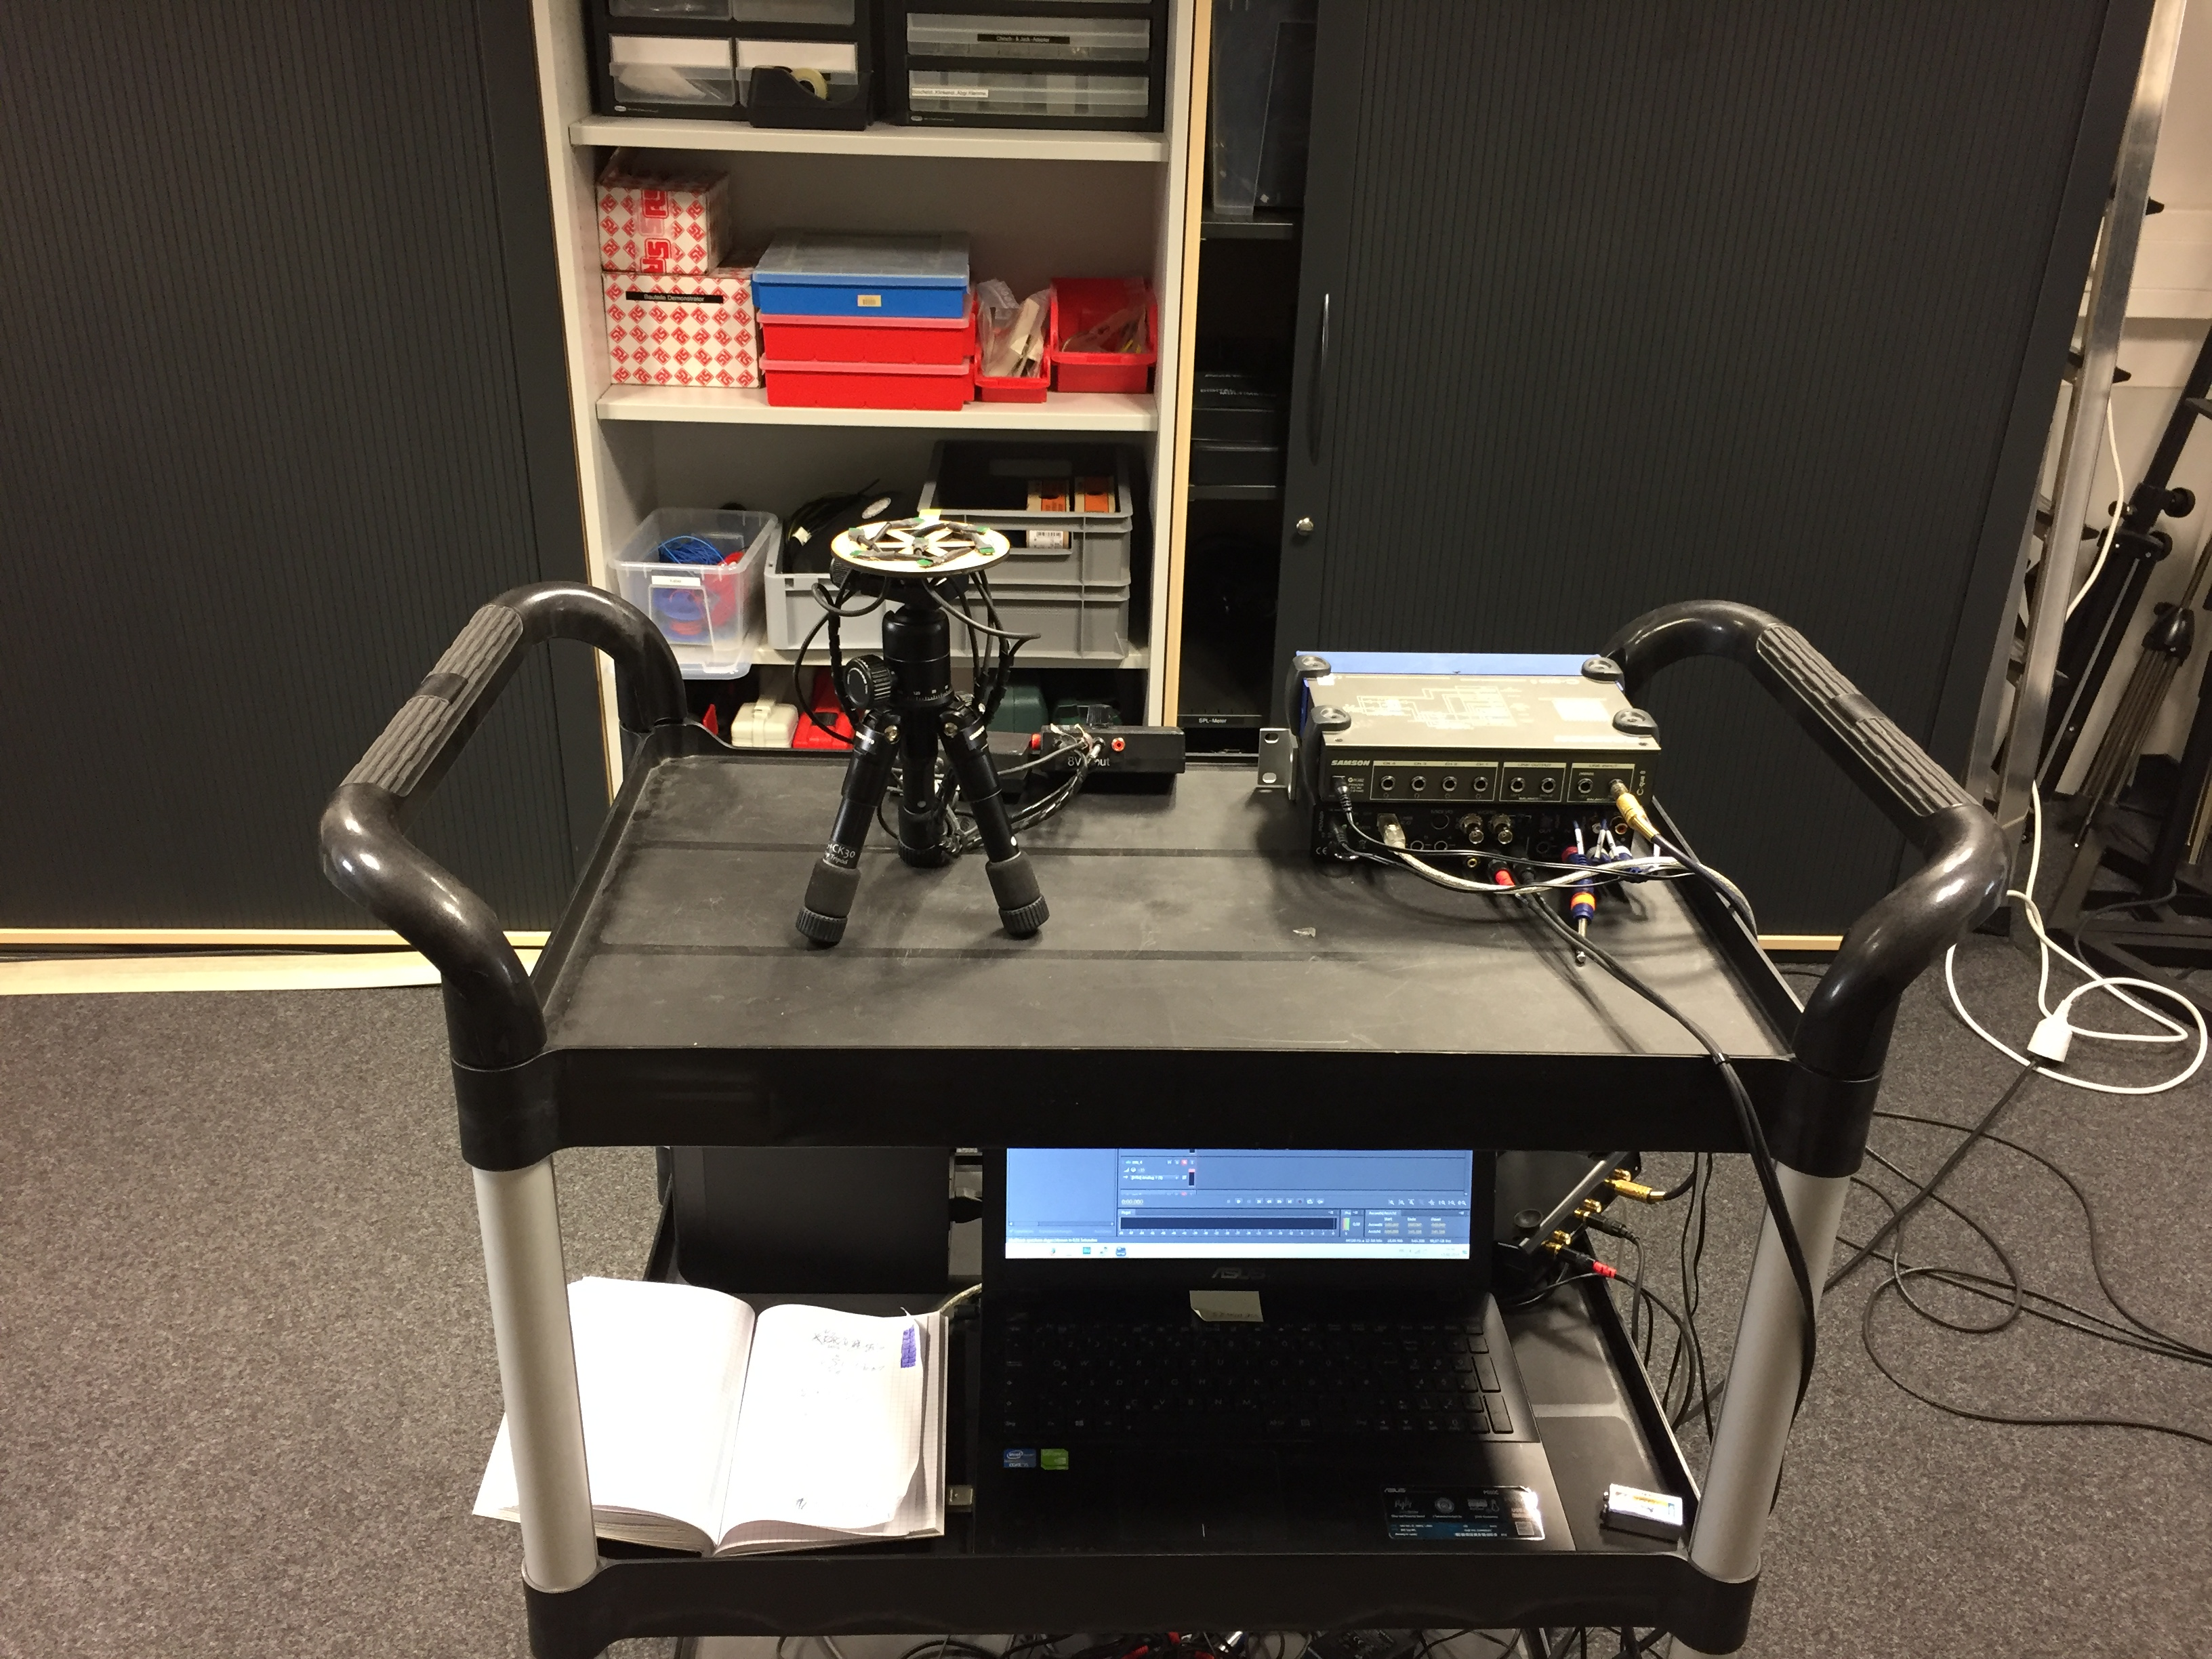
\includegraphics[width=0.8\textwidth]{figures/mic_rec_setup.jpg}
	\caption{Microphone signal recording setup}
	\label{fig:mic_rec_setup}
\end{figure}

\begin{figure}[!ht]
	\centering
	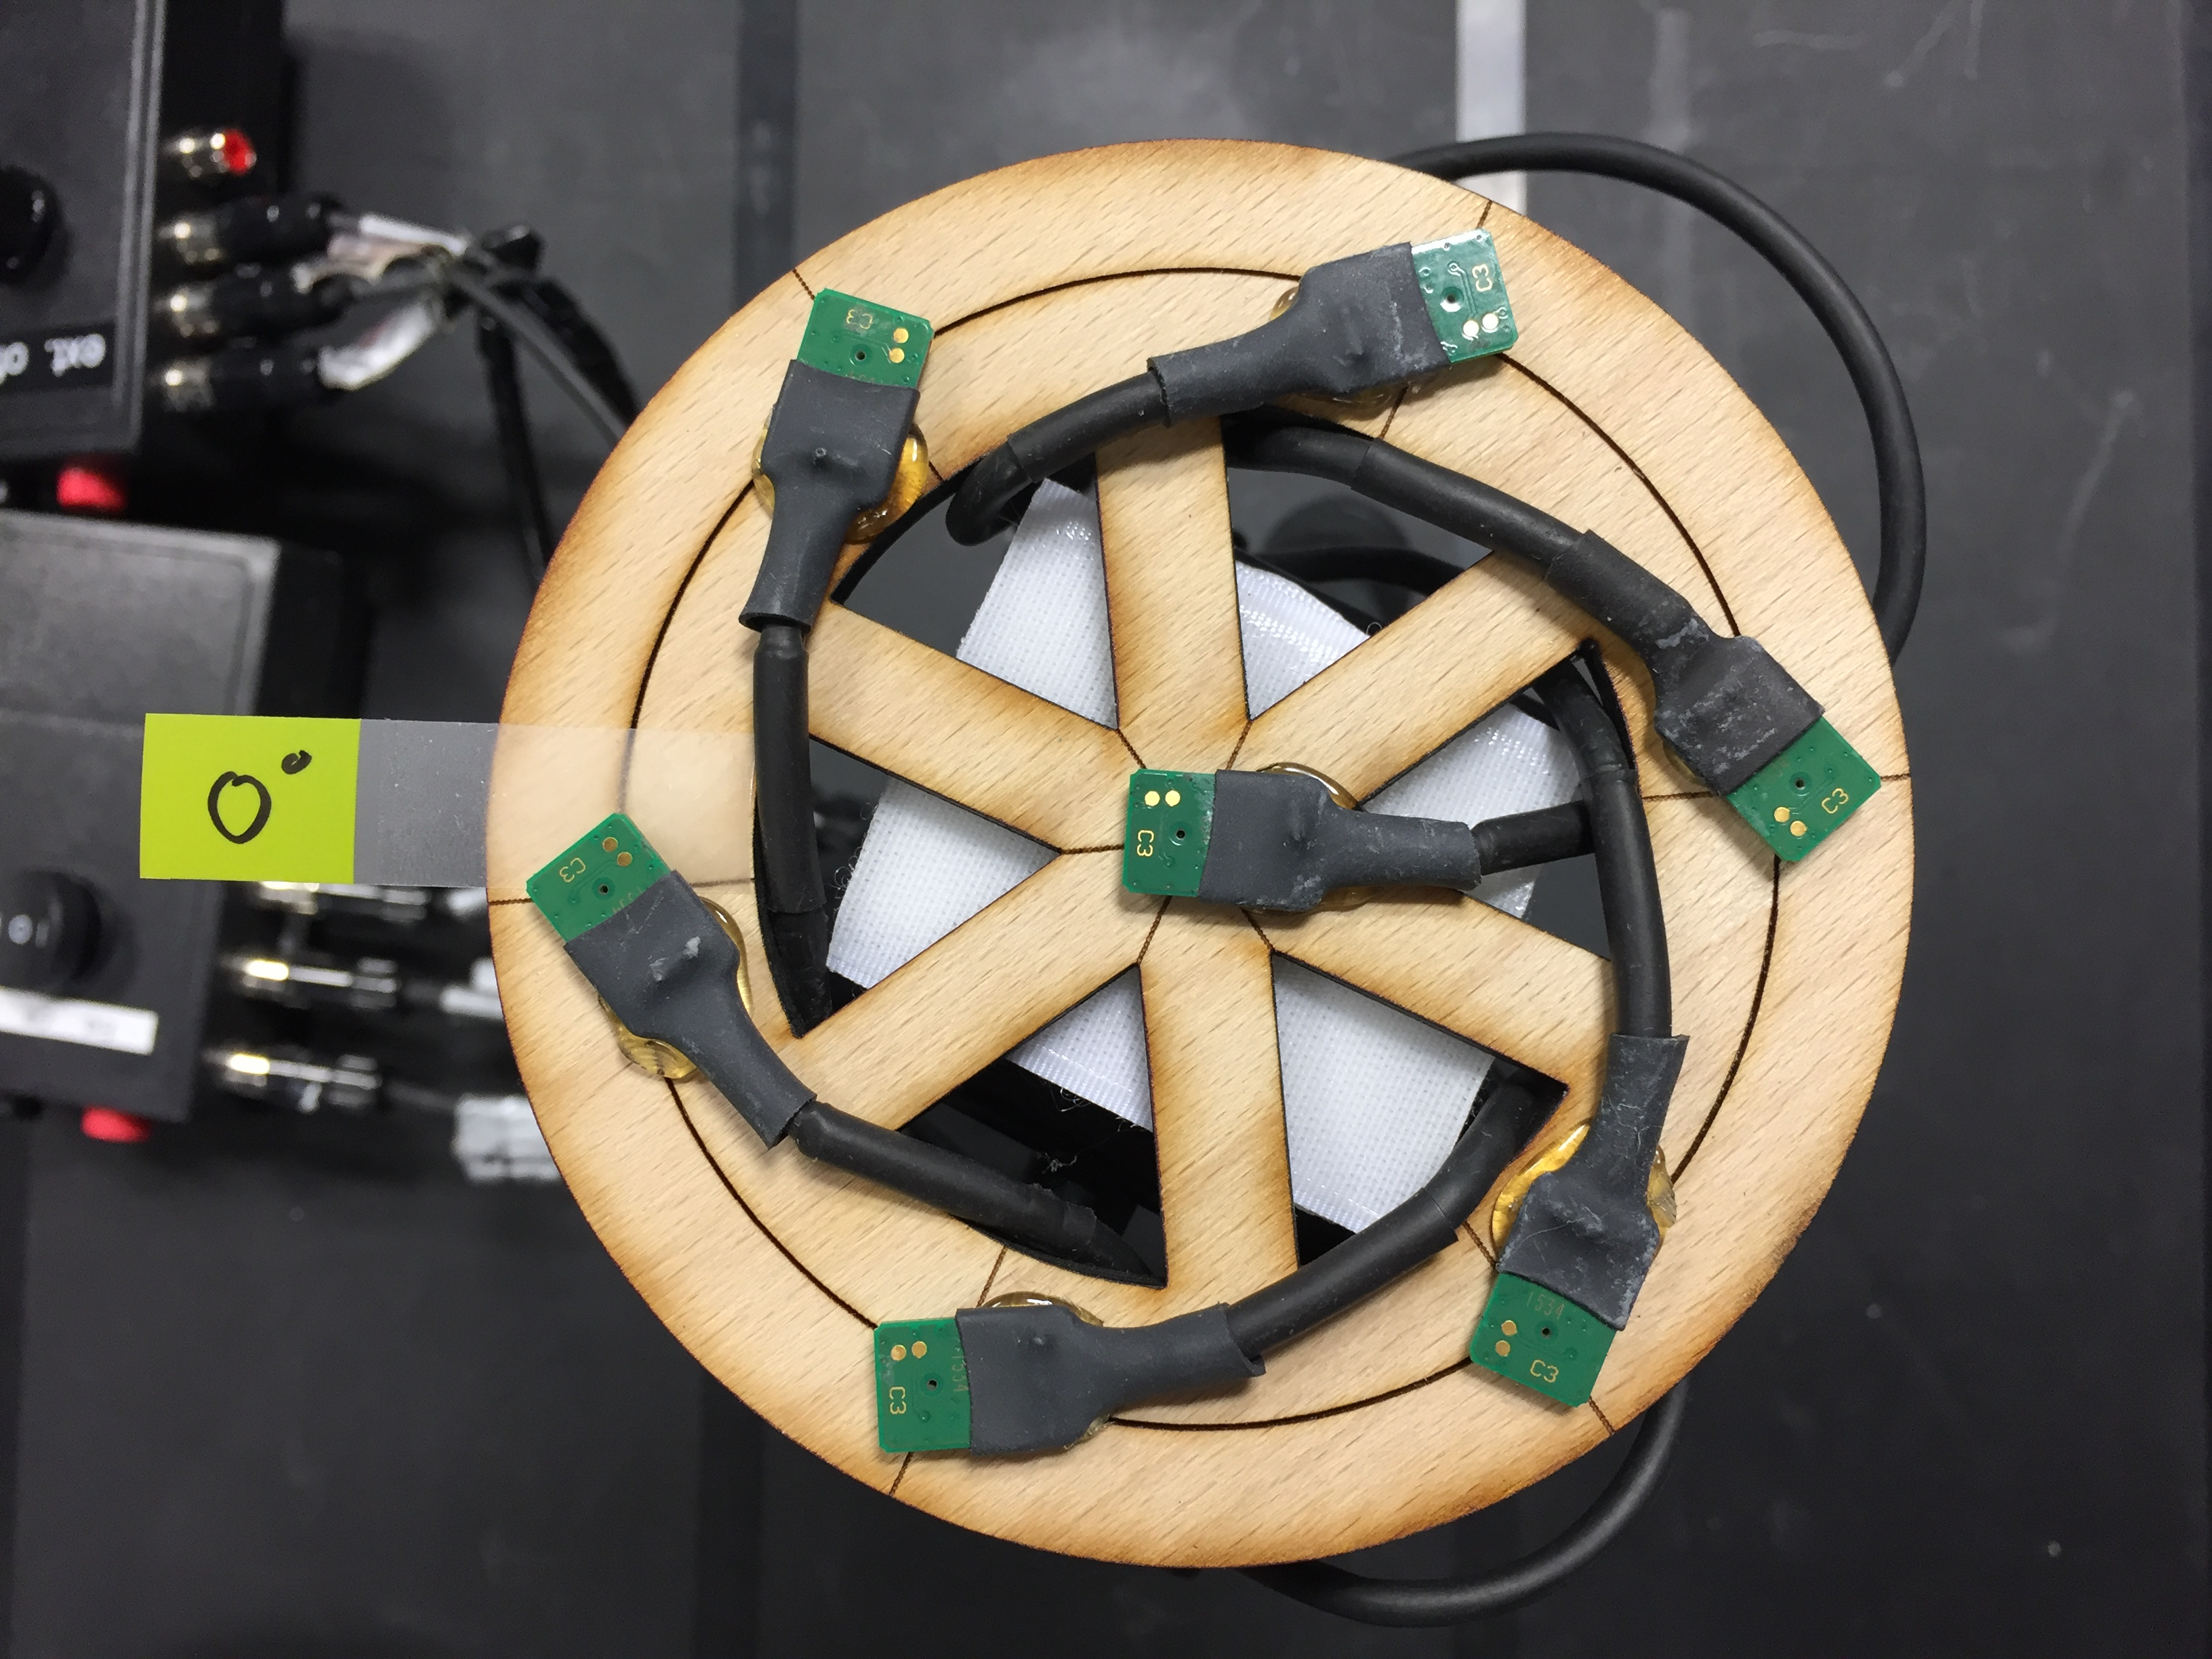
\includegraphics[width=0.8\textwidth]{figures/mic_array_foto.jpg}
	\caption{Foto of the used 7 microphone Uniform circular array with center microphone}
	\label{fig:mic_array}
\end{figure}

\begin{figure}[!ht]
	\centering
	\includegraphics[width=0.8\textwidth]{figures/label_tool.PNG}
	\caption{Labeling Tool}
	\label{fig:label_tool}
\end{figure}


\begin{figure}[!ht]
	\centering
	\begin{minipage}[!ht]{.49\textwidth}
		  \def\svgwidth{1\linewidth}
		  \small\input{figures/scenario_1.pdf_tex}
		\caption{Ground truth over time for scenario 1}
		\label{fig:scenario1}
	\end{minipage}%
	\hfill
	\begin{minipage}[!ht]{.49\textwidth}
		\centering
		\def\svgwidth{1\linewidth}
		\input{figures/scenario_2.pdf_tex}
		\caption{Ground truth over time for scenario 2}
		\label{fig:scenario2}
	\end{minipage}
\end{figure}

\begin{figure}[!ht]
	\centering
	\begin{minipage}[!ht]{.49\textwidth}
		  \def\svgwidth{1\linewidth}
		  \small\input{figures/scenario_3.pdf_tex}
		\caption{Ground truth over time for scenario 3}
		\label{fig:scenario3}
	\end{minipage}%
	\hfill
	\begin{minipage}[!ht]{.49\textwidth}
		\centering
		\def\svgwidth{1\linewidth}
		\input{figures/scenario_4.pdf_tex}

		\caption{Ground truth over time for scenario 4}
		\label{fig:scenario4}
	\end{minipage}
\end{figure}

\begin{figure}[!ht]
	\centering
	\begin{minipage}[!ht]{.49\textwidth}
		  \def\svgwidth{1\linewidth}
		  \small\input{figures/scenario_5.pdf_tex}
		\caption{Ground truth over time for scenario 5}
		\label{fig:scenario5}
	\end{minipage}%
	\hfill
	\begin{minipage}[!ht]{.49\textwidth}
		\centering
		\def\svgwidth{1\linewidth}
		\input{figures/scenario_6.pdf_tex}

		\caption{Ground truth over time for scenario 6}
		\label{fig:scenario6}
	\end{minipage}
\end{figure}

\begin{figure}[!ht]
		\centering
		\def\svgwidth{0.5\linewidth}
		\small\input{figures/scenario_7.pdf_tex}
		\caption{Ground truth over time for scenario 7}
		\label{fig:scenario7}
\end{figure}

\begin{table}[!ht]
\centering
\begin{tabular}{lll}
\toprule
\# 			& Development Set                                              \\ \midrule

D1         & One source moving around the array while speaking                                                                                                      \\
D2         & One source speaks successively from three positions                                                                                                \\
D3         & Two sources from fixed positions speaking successively                                                                                              \\
D4         & \begin{tabular}[c]{@{}l@{}}One fixed permanent music source, one moving source permanently speaking\\   with crossover\end{tabular}             \\
D5         & \begin{tabular}[c]{@{}l@{}}Two sources at $\ang{45}$  azimuth plane\\ alternately speaking first then at the same time\end{tabular}              \\
D6         & One source saying a wake-up-word moves and then asks a question                                                                                       \\
D7         & One source saying a wake-up-word and then asks a question while music is playing                                                                                              \\ \bottomrule
           &                                                                                                                                                    \\
           \toprule
\#         & Evaluation Set                                                                                                                                     \\ \midrule
E1         & Two fixed sources at $\ang{90}$ azimuth plane both simultaneously speaking                                                                                    \\
E2         & One fixed source, one moving source speaking simultaneously                                                                                           \\
E3         & \begin{tabular}[c]{@{}l@{}}One fixed source continuously speaking, one moving source speaking wake-up-\\   words from different directions\end{tabular} \\
E4         & Two sources moving and speaking simultaneously, no crossovers                                                                                       \\
E5         & Two sources moving and speaking simultaneously with crossovers                                                                                      \\
E6         & \begin{tabular}[c]{@{}l@{}}Three static sources continuously speaking with minimum $\ang{80}$ azimuth plane\\   distance\end{tabular}                       \\
E7         & \begin{tabular}[c]{@{}l@{}}Three static sources continuously speaking with minimum $\ang{40}$ azimuth plane\\   distance\end{tabular}     					\\
\bottomrule
\end{tabular}
\caption{List of descriptions of all scenarios used for development and evaluation set}
\label{tab:list_scenario}
\end{table}


\begin{table}[!ht]
\centering
\begin{tabular}{l|ll|ll} \toprule
                       & \multicolumn{2}{l}{Broadband SRP} & \multicolumn{2}{l}{Sub-band SRP} \\ \midrule
Parameter              & Delay and Sum       & Capon       & Delay and Sum       & Capon      \\ \midrule
Circular buffer length $N$ & 16                  & 16          & 257                 & 257        \\
Hypothesis threshold $\Gamma_\text{class}^\text{add}$  & 7                   & 8           & 50                  & 20         \\
PDF Floor class $p_\text{floor}$           & 0.0001              & 0.0001      & 0.01                & 0.001      \\
MAP-Adaption par.  $\beta$               & 40                  & 50          & 50                  & 10         \\
Min. mixing coef. $\Gamma^\text{min}_\text{mix}$             & 0.01                & 0.001       & 0.01                & 0.01       \\
Variance $\sigma^2_\text{const}$        & $13^2$                  & $14^2$          & $10^2$                  & $10^2$         \\
Initial TTL value $b_\text{TTL}^\text{add}$      & 30                  & 30          & 50                  & 50         \\
TTL Threshold  $\Gamma^\text{TTL}_\text{thres}$        & 0.01                & 0.01        & 0.01                & 0.01       \\
TTL increase  $b_\text{TTL}^\text{inc}$              & 30                  & 30          & 8                   & 8          \\
TTL maximum  $\Gamma_\text{TTL}^\text{max}$              & 20                  & 20          & 15                  & 15         \\
Overlap Distance $\Gamma_\text{overlap}$      & 40                  & 40          & 40                  & 40         \\
Aliasing Distance  $\Gamma_\text{al}$    & -                   & -           & 15                  & 15        \\
\bottomrule
\end{tabular}
\caption{Parameters for the different developed multi-source classification algorithm}
\label{tab:para_alg}
\end{table}

\begin{table}[!ht]
\centering

\begin{tabular}{l|l}
\toprule
Parameter Name            & Value \\\midrule
Buffer Length   $N$          & 257   \\
Number of initial sources $K_\text{init}$ & 5     \\
Initial TTL $b_\text{TTL}^\text{init}$              & 2     \\
TTL increase $b_\text{TTL}^\text{inc}$             & 12    \\
TTL maximum  $\Gamma_\text{TTL}^\text{max}$              & 20\\
Threshold Affiliations $\Gamma_\text{affil}$   & 70    \\
Floor class   $p_\text{floor}$            & 0.001 \\
Overlap distance  $\Gamma_\text{overlap}$        & 40    \\
\bottomrule
\end{tabular}
\caption{Parameters for Madhu's multi-source classification algorithm}
\label{tab:para_madhu}
\end{table}


\begin{figure}[!ht]
		\centering
		\def\svgwidth{1\linewidth}
		\small\input{figures/results_idc_example1_comp.pdf_tex}
		\caption{Scenario E7, processed with the developed sub-band algorithm with a Capon beamformer}
		\label{fig:results_idc_ex1_comp}
\end{figure}

\begin{figure}[!ht]
	\subfloat[Broadband processing\label{fig:results_comp_ex2}]{%
		  \def\svgwidth{.49\linewidth}
		  \small\input{figures/results_comp_example2.pdf_tex}
	}
	\hfill
	\subfloat[Sub-band processing\label{fig:results_comp_ex3}]{%
		  \def\svgwidth{.49\linewidth}
		  \small\input{figures/results_comp_example3.pdf_tex}
	}
	\caption{Active system track values over time are shown. Sub-band processing has more active system track values than the broadband processing.}
	\label{fig:results_comp_bb_vs_sb}
\end{figure}

\begin{table}[!ht]
\centering
\begin{tabular}{l|ll|ll|l}
\toprule
      & BB D\&S & BB CAP & SB D\&S & SD CAP & MADHU \\ \midrule
E1    & 0       & 0      & 0       & 0      & 0     \\
E2    & 0       & 0      & 0       & 0      & 0     \\
E3    & 0       & 0      & 0       & 0      & 2     \\
E4    & 0       & 0      & 0       & 0      & 0     \\
E5    & 8       & 6      & 6       & 6      & 6     \\
E6    & 0       & 0      & 0       & 0      & 0     \\
E7    & 8       & 10     & 0       & 0      & 0     \\ \midrule
Total & 16      & 16     & 6       & 6      & 8    \\
\bottomrule
\end{tabular}
\caption{ID changes for all scenarios and algorithms}
\label{tab:idc}
\end{table}

\begin{table}[!ht]
\centering
\begin{tabular}{l|ll|ll|l}
\toprule
      & BB D\&S & BB CAP & SB D\&S & SD CAP & MADHU \\\midrule
E1    & $\ang{3.46 }$   & $\ang{2.86 }$  & $\ang{3.18 }$   & $\ang{3.35 }$  & $\ang{3.35 }$ \\
E2    & $\ang{4.66 }$   & $\ang{4.09 }$  & $\ang{3.64 }$   & $\ang{3.71 }$  & $\ang{5.08 }$ \\
E3    & $\ang{2.78 }$   & $\ang{3.64 }$  & $\ang{1.26 }$   & $\ang{2.05 }$  & $\ang{4.87 }$ \\
E4    & $\ang{4.84 }$   & $\ang{5.09 }$  & $\ang{4.08 }$   & $\ang{3.26 }$  & $\ang{2.89 }$ \\
E5    & $\ang{13.15}$   & $\ang{14.37}$  & $\ang{8.73 }$   & $\ang{9.68 }$  & $\ang{9.42 }$ \\
E6    & $\ang{2.17 }$   & $\ang{2.17 }$  & $\ang{2.45 }$   & $\ang{2.85 }$  & $\ang{3.74 }$ \\
E7    & $\ang{9.69 }$   & $\ang{8.32 }$  & $\ang{1.87 }$   & $\ang{1.99 }$  & $\ang{8.43 }$ \\ \midrule
Total & $\ang{7.62 }$   & $\ang{7.95 }$  & $\ang{4.32 }$   & $\ang{4.92 }$  & $\ang{6.3  }$\\ \bottomrule
\end{tabular}
\caption{Root mean square error values for all scenarios and algorithms}
\label{tab:rmse}
\end{table}

\begin{table}[!ht]
\centering

\begin{tabular}{l|ll|ll|l}
\toprule
      & BB D\&S & BB CAP & SB D\&S & SD CAP & MADHU \\ \midrule
E1    & 1.77    & 2.02   & 0.09    & 0.58   & 0.05  \\
E2    & 0.27    & 0.29   & 0.08    & 0.08   & 0.08  \\
E3    & 0.28    & 0.22   & 0.15    & 0.16   & 0.15  \\
E4    & 0.16    & 0.14   & 0.02    & 0.03   & 0     \\
E5    & 0       & 0      & 0.13    & 0      & 0     \\
E6    & 1.42    & 1.38   & 0.19    & 0.04   & 0.04  \\
E7    & 0.14    & 0.19   & 0       & 0      & 0     \\ \midrule
Total & 0.56    & 0.59   & 0.08    & 0.1    & 0.03  \\ \bottomrule
\end{tabular}
\caption{Initial detection lag in seconds for all scenarios and algorithms}
\label{tab:lag}
\end{table}


\begin{table}[!ht]
\centering
\begin{tabular}{l|ll|ll|l}
\toprule
      & BB D\&S & BB CAP & SB D\&S & SD CAP & MADHU \\\midrule
E1    & 0     & 0      & 0     & 0      & 0     \\
E2    & 0     & 0      & 0     & 0      & 0     \\
E3    & 0     & 0      & 0     & 0      & 0     \\
E4    & 0     & 0      & 0     & 0      & 0     \\
E5    & 1     & 1      & 2     & 2      & 1     \\
E6    & 0     & 0      & 0     & 0      & 0     \\
E7    & 0     & 0      & 0     & 0      & 0     \\ \midrule
Total & 1     & 1      & 2     & 2      & 1    \\
\bottomrule
\end{tabular}
\caption{Interrupt values for all scenarios and algorithms}
\label{tab:interrupts}
\end{table}

\begin{table}[!ht]
\centering
\begin{tabular}{l|ll|ll|l}
\toprule
      & BB D\&S & BB CAP & SB D\&S & SD CAP & MADHU \\ \midrule
E1    & 0       & 0      & 0       & 0      & 0.03  \\
E2    & 0       & 0      & 0       & 0      & 0.43  \\
E3    & 7.1     & 1.66   & 7.06    & 5.9    & 9.79  \\
E4    & 0       & 0      & 0       & 0      & 0     \\
E5    & 0       & 0      & 0       & 1.12   & 0.03  \\
E6    & 0       & 0      & 0.67    & 0.43   & 1.7   \\
E7    & 0       & 0      & 0.5     & 0      & 0.45  \\ \midrule
Total & 7.1     & 1.66   & 8.22    & 7.46   & 12.43   \\
\bottomrule
\end{tabular}
\caption{False positive durations in seconds for all scenarios and algorithms}
\label{tab:fp}
\end{table}

\end{appendix}

                %%% Anhang (Optional, ggf ändern)

%\printglossary          				%%% GLosar (Optional!)
%\printindex             				%%% Index (Optional!)


\end{document}
